\documentclass[11pt,twoside]{report}
%%%%%%%%%%%%%%%%%%%%

\input{packages}
%%%%%%%%%%%%%%%%%%%%%%%%%%%%%%%%%%%%%%%%%%%%
\hypersetup{pdftitle = Report, pdfauthor = {First Last}, pdfstartview=FitH, pdfkeywords = essay, pdfpagemode=FullScreen, colorlinks, anchorcolor = red, citecolor = blue,urlcolor=teal, filecolor=green, linkcolor=codepurple, plainpages=false}
%%%%%%%%%%%%%%%%%%%%%%%%%%%%%%%%%%%%%%%%%%%%%%%%%%%%%%%%%%%%%%%%%%%%%%%
\newlength{\bibitemsep}\setlength{\bibitemsep}{.2\baselineskip plus .05\baselineskip minus .05\baselineskip}
\newlength{\bibparskip}\setlength{\bibparskip}{0cm}
\let\oldthebibliography\thebibliography
\renewcommand\thebibliography
\oldthebibliography
  \setlength{\parskip}{\bibitemsep}
  \setlength{\itemsep}{\bibparskip}
%setmainfont{TeX Gyre Pagella}

%%%%%%%%%%%%%%%%%%%%%%%%55
\usepackage{fancyhdr}
\pagestyle{fancy}
\fancyhf{}   % clear everything

% ---------- Marks ----------
\renewcommand{\chaptermark}[1]{%
  \markboth{#1}{}}


\renewcommand{\sectionmark}[1]{%
  \markright{\quad #1}}

% ---------- Header Layout ----------
% Even pages (left pages)
\fancyhead[LE]{\textbf{\thepage}}                     % page number left
\fancyhead[RE]{\nouppercase{\leftmark}}      % chapter title centered

% Odd pages (right pages)
\fancyhead[LO]{\nouppercase{\rightmark}}     % section title left
\fancyhead[RO]{\textbf{\thepage}}                     % page number right

% ---------- Lines ----------
\renewcommand{\headrulewidth}{0.4pt}
\renewcommand{\footrulewidth}{0pt}


\newcommand{\starredline}{\leavevmode\xleaders\hbox{\makebox[1em]{\hss$\star$\hss}}\hfill\kern0pt}

 
% Line spacing
\renewcommand{\baselinestretch}{1.05} %1.5

%Line with star at the end of the week.
\newcommand{\stardivider}{
\noindent\hrulefill\quad$\displaystyle ***$\quad\hrulefill 
}

%%%%%%%%%%%%%%%%%%%%%%%%%%%%%%%%%%%%%%%%%%%%%%%%%%%%%%%%%%%%%%%%%%%%%%%%%%%%%%%%%%%%
\title{\Huge{ RESEARCH JOURNAL - 2026}}
\author{\\ \LARGE{Pravin Sharma}
\\ 5$^{th}$ Year, Ph.D. Student
\\ 
\\
\vspace{6.5cm}
\\
\\
\\
\\ Department of Applied Science \\ William \& Mary
\\
\\ 
%\\November 2022
}
%\date{November 2022}
\date{\Huge{2026}}

%%%%%%%%%%%%%%%%%%%%%%%%%%%%%%%%%%%%%%%%%%%%%%%%%%%%%%%%%%%%%%%%%%%%%%%
\cleardoublepage
% \endtit

\newcommand{\cmark}{\textcolor{green}{\textbf{\Large\ding{51}}}}  % ✓
\newcommand{\xmark}{\textcolor{red}{\textbf{\Large\ding{55}}}} % X
\newcommand{\qmark}{\textcolor{blue}{\textbf{\Large?}}}

\begin{document}
\sloppy
\thispagestyle{headings}
\maketitle


% \FloatBarrier
\pagenumbering{roman}
% \chapter*{Preface}
% \input{preface.tex}

% \newpage
%\pagenumbering{roman}
\cleardoublepage

\newpage
\tableofcontents
\thispagestyle{plain}
% \listoffigures
% \listoftables

% Include the list of abbreviations here if required.
\newpage
\pagenumbering{arabic}


\newpage

\setcounter{section}{0}


% \chapter{January}
\label{chap:Jan}


These section will include the details of the task related to my research which I have done in the month of January.
\paragraph{I have to make a folder with the input files and all details of each of the calculations which I have done. \hl{Basically organizing the input files.}}

The \hl{strong skill}s for January and February is completing the Machine Learning Course by Vizuara from YouTube \href{https://youtube.com/playlist?list=PLPTV0NXA_ZSiLI0ZfZYbHM2FPHKIuMW6K&si=ahBRjJkP5Mmh6D88}{Foundations of Machine Learning}

% % \section{Week - 01 }
\begin{physicsmodule}{Jan 01 - Jan 04}{RoyalBlue}
  \begin{lawbox}
    \subsection*{\sffamily\bfseries \textbf{Week - 01}}
    \begin{enumerate}
    \item Go to Hindu Center Richmond with Wife for Kirtan and blessed beginning of the year. \cmark  
    \item Get the required Indian Grocery if needed. \cmark
    \item See if all the simulations are completed for 22nm and 27 nm [Mon]. 
    \item Make the Gym plan for the semester. \cmark
    \item Plan the scanning of MSc certificates [Mon]. 
    \item Get the Reference code for the WES application [Mon].
    \item Complete the new plots for thickness and temperature for $\alpha_{\mathrm{eff}}$ and then write up the Results and Discussion for this [Tue].
    \item Make the files for 35nm onwards simulations and run it in the HPC, all at once [Wed].
    \item Text Mayank jee and go in evening and collect the money and tell him that you won't continue [Mon].
    \item Complete the 3 section of the Newton's Third law notes [Thu].    
\end{enumerate}
  \end{lawbox}
\end{physicsmodule}
\subsection*{\underline{Thursday Jan 01, 2026} -  \textcolor{red}{\Large{Happy New Year !!!}}}
\subsection*{To do Tasks:}
\begin{enumerate}
    \item Go to ISKCON Richmond with Wife for Kirtan and blessed beginning of the year. 
    \item Get the required Indian Grocery if needed.
    \item Complete the dual frequency fit and make the schematic draft of the paper of mine. 
\end{enumerate}
\subsection*{Completed Tasks}
\begin{enumerate}[\ding{52}]  % You can change the number to any dingbat symbol you want
    \item 
\end{enumerate}
\subsection*{Notes:}
\begin{enumerate}
    \item 
\end{enumerate}
%%%%%%%%%%%%%%%%%%%%%%%%%%%%%%%%%%%%%%%%%%%%%%%%%%%%%%%%%%%%%%%%%
\subsection*{\underline{Friday Jan 02, 2026}}
\subsection*{To do Tasks:}
\begin{enumerate}
    \item Read more about the PSSW papers.
    \item 
\end{enumerate}

\subsection*{Completed Tasks}
\begin{enumerate}[\ding{52}]  % You can change the number to any dingbat symbol you want
    \item 
\end{enumerate}
\subsection*{Notes:}
\begin{enumerate}
    \item Spin wave: A wave of quantized
\end{enumerate}
%%%%%%%%%%%%%%%%%%%%%%%%%%%%%%%%%%%%%%%%%%%%%%%%%%%%%%%%%%%%%%%%%
\subsection*{\underline{Saturday Jan 03, 2026}}
\subsection*{To do Tasks:}
\begin{enumerate}
    \item Go to airport and see off wife to Boston. Plan the next trip after the GRS-2026 to visit her and take the tickets after getting next paycheck.
    \item Arrange the documents and see if you have scanned copies or not, if not then go to department and then get them scanned. 
    \item Go to gym after talking with wife and then get fresh and start doing the work for this. 
    \item Complete the reading of these 3 papers related to PSSW with basic understanding cleared. 
    \item Watch 1 hour of LinkedIn Learning for python course completion.
\end{enumerate}
\subsection*{Completed Tasks}
\begin{enumerate}[\ding{52}]  % You can change the number to any dingbat symbol you want
    \item 
\end{enumerate}
\subsection*{Notes:}
\begin{enumerate}
    \item 
\end{enumerate}
% %%%%%%%%%%%%%%%%%%%%%%%%%%%%%%%%%%%%%%%%%%%%%%%%%%%%%%%%%%%%%%%%%
\subsection*{\underline{Sunday Jan 04, 2026} }
\subsection*{To do Tasks:}
\begin{enumerate}
    \item Pay to the IRS first. \cmark
    \item Complete the reading of PSSW papers.
\end{enumerate}
\subsection*{Completed Tasks}
\begin{enumerate}[\ding{52}]  % You can change the number to any dingbat symbol you want
    \item 
\end{enumerate}
\subsection*{Notes:}
\begin{enumerate}
    \item 
\end{enumerate}
\starredline
%%%%%%%%%%%%%%%%%%%%%%%%%%%%%%%%%%%%%%%%%%%%%%%%%%%%%%%%%%%%%%%%%




% % \input{Months/1. January/PSSW_papers}
% % \section{Week - 02}
\begin{physicsmodule}{Jan 05 - Jan 10}{RoyalBlue}
  \begin{lawbox}
    \subsection*{\sffamily\bfseries Week - 02}
    \begin{enumerate}
    \item Design and make the file for CoFe/FeO material. First make and visualize it before running any other calculations [Wed].
    \item List the calculations which needs to be done [Tue].
    \item See the details as shared by Sid Mitra and prepare the requirements for the Boot Camp [Tue]. 
    \item Complete the WES application for the MSc Physics and share the document to Karthik and add Sanjay brother in the group [Mon] \cmark.
    \item Complete the reading for the PSSW papers [Tue] and think of making files[Wed]. 
    \item Re-run the simulations whose data are not there [Mon]. 
    \item Call Mack in the evening [Tue].
    \item Complete one video of ML YouTube Video [Thu].
\end{enumerate}
  \end{lawbox}
\end{physicsmodule}
%%%%%%%%%%%%%%%%%%%%%%%%%%%%%%%%%%%%%%%%%%%%%%%%%%%%%%%%%%%%%%%%%
\subsection*{\underline{Monday Jan 05, 2026}}
\subsection*{To do Tasks:}
\begin{enumerate}
    \item Pay the Natural Gas and WiFi bill if appeared on Credit card. \cmark 
    \item Share the copy of mark sheet to Kartik and share the WES reference code later in the day after WES thing. \cmark
    \item Watch two videos and make the notes sidewise from \ref{chap:Magnetism} channel. \cmark
    \item Complete the PSSW papers reading.\xmark
    \item Submit the data not available simulations and make the thicknesses for high ones and double check the files. \xmark 
    \item Re-read the basics and ideas about the VIMS Presentation Bootcamp. \xmark
\end{enumerate}
% \subsection*{Completed Tasks}
% \begin{enumerate}[\ding{52}]  % You can change the number to any dingbat symbol you want
%     \item 
% \end{enumerate}
\subsection*{Notes:}
\begin{enumerate}
    \item Day was good but, didn't had much things to do and completed 2 different videos for Magnetism basics.
\end{enumerate}
%%%%%%%%%%%%%%%%%%%%%%%%%%%%%%%%%%%%%%%%%%%%%%%%%%%%%%%%%%%%%%%%%
\subsection*{\underline{Tuesday Jan 06, 2026}}
\subsection*{To do Tasks:}
\begin{enumerate}
 \item Read the PSSW papers before lunch and make notes for them. \cmark
    \item Gather the details about the VIMS' STEM teaching boot camps.\cmark
    \item Work on the presentation related to the same. \xmark
    \item Make the files whose data are not available, and make the files for the other jobs which needs to be submitted again after the 8th Jan. \xmark
    \item Go to watch the Avatar:Fire and Ash movie at evening around 5:30 pm and take the car. \cmark
\end{enumerate}
\subsection*{Completed Tasks}
\begin{enumerate}[\ding{52}]  % You can change the number to any dingbat symbol you want
    \item Went to lab for some time but came early and did the rest work in the home. 
\end{enumerate}
% \subsection*{Notes:}
% \begin{enumerate}
%     \item 
% \end{enumerate}
%%%%%%%%%%%%%%%%%%%%%%%%%%%%%%%%%%%%%%%%%%%%%%%%%%%%%%%%%%%%%%%%%
\subsection*{\underline{Wednesday Jan 07, 2026} }
\subsection*{To do Tasks:}
\begin{enumerate}
    \item Complete the PSSW paper reading.\cmark
    \item Work the rest of the day on the VIMS Boot Camp thing. \xmark
    \item Go and get the money from Mayank jee.\cmark
    \item Order the iPad case.\cmark
    \item Work on files for simulations.\xmark
    \item Watch 1 video of Magnetism basics by channel Gyan Sampada. \xmark
\end{enumerate}
\subsection*{Completed Tasks}
\begin{enumerate}[\ding{52}]  % You can change the number to any dingbat symbol you want
    \item Got the money from Mayank jee and had a good terms while cancelling the work.
\end{enumerate}
% \subsection*{Notes:}
% \begin{enumerate}
%     \item 
% \end{enumerate}
% %%%%%%%%%%%%%%%%%%%%%%%%%%%%%%%%%%%%%%%%%%%%%%%%%%%%%%%%%%%%%%%%%
\subsection*{\underline{Thursday Jan 08, 2026}}
\subsection*{To do Tasks:}
\begin{enumerate}
    \item Complete the reading of the PSSW papers. \cmark
    \item Submit the simulations for the folder whose data is not present. [t100 and t200]. \cmark
    \item Watch 1 video of Magnetism basics by Gyan Sampada channel.
    \item Go and get the bedsheets for the bootcamp from Walmart. \cmark
\end{enumerate}
\subsection*{Completed Tasks}
\begin{enumerate}[\ding{52}]  % You can change the number to any dingbat symbol you want
    \item Submitted the simulations for the 100 and 200 K as their data was missing and then will re do the fitting and all things.
\end{enumerate}
% \subsection*{Notes:}
% \begin{enumerate}
%     \item 
% \end{enumerate}
% %%%%%%%%%%%%%%%%%%%%%%%%%%%%%%%%%%%%%%%%%%%%%%%%%%%%%%%%%%%%%%%%%
\subsection*{\underline{Friday Jan 09, 2026}}
\subsection*{To do Tasks:}
\begin{enumerate}
    \item Work on the completing the Preworkshop questionnarie for the Boot Camp thing before lunch. \cmark  
    \item Complete the paper of PSSW reading after doing this above one task. \cmark
    \item Make the files separately for each temperature for high thicknesses to get the PSSW modes. \xmark
    \item Go on walk with Yicheng if he shows up. \cmark
    \item Come back from walk and then spend 2 hours in learning the Magnetism basics videos from Gyan Sampada.\xmark
\end{enumerate}
\subsection*{Completed Tasks}
\begin{enumerate}[\ding{52}]  % You can change the number to any dingbat symbol you want
    \item Shared the pdf of PSSW Papers in onedrive and can read that later to revise from iPad. 
\end{enumerate}
% \subsection*{Notes:}
% \begin{enumerate}
%     \item 
% \end{enumerate}
% %%%%%%%%%%%%%%%%%%%%%%%%%%%%%%%%%%%%%%%%%%%%%%%%%%%%%%%%%%%%%%%%%
\subsection*{\underline{Saturday Jan 10, 2026} }
\subsection*{To do Tasks:}
\begin{enumerate}
    \item Collect the main points and do pack the bag gently with all the required things at night.
    \item Revise the work of whole week and plan ahead the next week and important tasks of the coming week. 
\end{enumerate}
% \subsection*{Completed Tasks}
% \begin{enumerate}[\ding{52}]  % You can change the number to any dingbat symbol you want
%     \item 
% \end{enumerate}
% \subsection*{Notes:}
% \begin{enumerate}
%     \item 
% \end{enumerate}
% %%%%%%%%%%%%%%%%%%%%%%%%%%%%%%%%%%%%%%%%%%%%%%%%%%%%%%%%%%%%%%%%%
\subsection*{\underline{Sunday Jan 11, 2026}}
\subsection*{To do Tasks:}
\begin{enumerate}
    \item Get ready for the VIMS Oral Boot camp 2026.
    \item Re-read the PSSW notes for the discussion with wife at 2:30 pm [\textcolor{blue}{Time changed to 3:00 pm because she was busy.}]. \cmark. 
    \item Prepare the talk for VIMS, note down the details on iPad. 
\end{enumerate}
\subsection*{Completed Tasks}
\begin{enumerate}[\ding{52}]  % You can change the number to any dingbat symbol you want
    \item 
\end{enumerate}
% \subsection*{Notes:}
% \begin{enumerate}
%     \item 
% \end{enumerate}
\starredline
% % \section{Week - 03}
\begin{physicsmodule}{Jan 11 - Jan 17}{RoyalBlue}
  \begin{lawbox}
    \subsection*{\sffamily\bfseries Week - 03}
    \begin{enumerate}
    \item Get ready for the Boot camp and do everything by 9:30 am. \cmark 
    \item make the rough notes and track them at VIMS-ESL and update them after coming back from the Boot camp [Fri-evening].
    \item Complete the new thicknesses inclusive plots and write the caption for them [Thu-all day].
    \item Work on writing the paper after submitting the large thickness based simulations for $\mathrm{No_{80}Fe_{20}}$ as per the paper of Panda et. al. \cite{pandaUltrafastDemagnetizationPrecession2023} [Friday all daytime].
    \item 
\end{enumerate}
  \end{lawbox}
\end{physicsmodule}
%%%%%%%%%%%%%%%%%%%%%%%%%%%%%%%%%%%%%%%%%%%%%%%%%%%%%%%%%%%%%%%%%
\subsection*{\underline{Sunday Jan 11, 2026}}
\subsection*{To do Tasks:}
\begin{enumerate}
    \item Complete the packing and go to VIMS Oral Bootcamp with Aidan. There is traveling and setting up for this Bootcamp this whole day. \cmark
\end{enumerate}
% \subsection*{Completed Tasks}
% \begin{enumerate}[\ding{52}]  % You can change the number to any dingbat symbol you want
%     \item 
% \end{enumerate}
\subsection*{Notes:}
\begin{enumerate}
    \item See the detailed things done and got from the VIMS Bootcamp in the goodnotes, Pravin/Notes-2026/Oral Bootcamp.
\end{enumerate}

% \newpage
% \section{2026 Oral Communication Bootcamp VIMS}
% The image which I have to present is,
% \begin{figure}[h!]
%     \centering
%     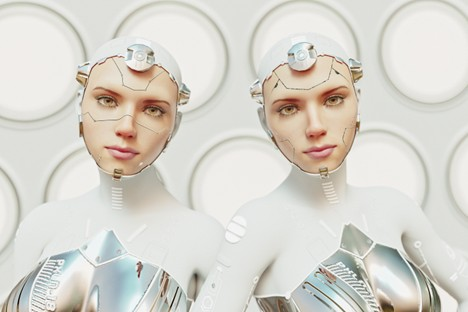
\includegraphics[width=0.95\linewidth]{Images/Pravin's pic for bootcamp.jpg}
%     \caption*{\textit{Image which Pravin Sharma is presenting in the 2026 VIMS Oral bootcamp}}
%     \label{fig:pravin-bootcamp-image}
% \end{figure}

% See the file in Goodnotes named 2026 Oral Communication Bootcamp inside January 2026. All the details are there.

%%%%%%%%%%%%%%%%%%%%%%%%%%%%%%%%%%%%%%%%%%%%%%%%%%%%%%%%%%%%%%%%%
% \subsection*{\underline{Monday Jan 12, 2026}}
% \subsection*{To do Tasks:}
% \begin{enumerate}
%     \item 
% \end{enumerate}
% \subsection*{Completed Tasks}
% \begin{enumerate}[\ding{52}]  % You can change the number to any dingbat symbol you want
%     \item 
% \end{enumerate}
% \subsection*{Notes:}
% \begin{enumerate}
%     \item 
% \end{enumerate}
% %%%%%%%%%%%%%%%%%%%%%%%%%%%%%%%%%%%%%%%%%%%%%%%%%%%%%%%%%%%%%%%%%
% \subsection*{\underline{Tuesday Jan 13, 2026}}
% \subsection*{To do Tasks:}
% \begin{enumerate}
%     \item  
% \end{enumerate}
% \subsection*{Completed Tasks}
% \begin{enumerate}[\ding{52}]  % You can change the number to any dingbat symbol you want
%     \item 
% \end{enumerate}
% \subsection*{Notes:}
% \begin{enumerate}
%     \item 
% \end{enumerate}
% %%%%%%%%%%%%%%%%%%%%%%%%%%%%%%%%%%%%%%%%%%%%%%%%%%%%%%%%%%%%%%%%%
\subsection*{\underline{Wednesday Jan 14, 2026} }
\subsection*{To do Tasks:}
\begin{enumerate}
    \item Read the papers and list the works which are supposed to be done in the remaining week.\cmark
\end{enumerate}
% \subsection*{Completed Tasks}
% \begin{enumerate}[\ding{52}]  % You can change the number to any dingbat symbol you want
%     \item 
% \end{enumerate}
% \subsection*{Notes:}
% \begin{enumerate}
%     \item 
% \end{enumerate}
%%%%%%%%%%%%%%%%%%%%%%%%%%%%%%%%%%%%%%%%%%%%%%%%%%%%%%%%%%%%%%%%%%
\subsection*{\underline{Thursday Jan 15, 2026}}
\subsection*{To do Tasks:}
\begin{enumerate}
    \item Complete the fitting for \hl{22 nm and 27 nm} for all temperatures and edit the final\_parameters table. \cmark 
    \item  PSSW waves calculations for the \hl{$\mathrm{Ni_{80}Fe_{20}}$} sample as per the paper \cite{pandaUltrafastDemagnetizationPrecession2023}.
    \begin{enumerate}[\ding{212}]
        \item The thicknesses which I am using in the benchmark simulation are only \hl{50nm and 100 nm} as per the paper.
        \item The structure is \hl{fcc, $T_c=863$K}.
        \item $\epsilon=0.790$, $z=12$, $J_{ij}=\frac{3k_BT_c}{\epsilon z}$ \\ where, $\epsilon$ is curative term derived from the mean field theory,\\ $z$ is the number of nearby atoms, \\ $T_c$ is the Curie temperature value, and \\ $k_B$ is the Boltzman constant which is $1.38\times10^{-23} J.K^{-1}$.
        \item The parameters which I have used in this simulations will be taken from the Richard Evan's paper \cite{evansAtomisticSpinModel2014}.
        \item The field application would be $15^\circ$ tilted out-of-plane (OOP).
        \item As per the external field application, which is $15^\circ$ tilted out-of-plane, the initial spin direction should also be || to the initial field. Hence, I am applying the initial spin direction as, 
        \[
        \begin{aligned}
            \mathbf{S}_0 &= (\sin\theta,\,0,\,\cos\theta) \\
            =\sin(15^\circ) &\approx 0.259 \\
            =\cos(15^\circ) &\approx 0.966 \\
            =>\mathbf{S}_0 &\approx (0.26,\,0,\,0.97)
        \end{aligned}
        \]  
        \item Submitted the simulations for \hl{$\mathrm{Ni_{80}Fe_{20}}$} for 50 nm and 100 nm.
    \end{enumerate}
\end{enumerate}
\subsection*{Completed Tasks}
\begin{enumerate}[\ding{52}]  % You can change the number to any dingbat symbol you want
    \item Completed the fitting for all the different temperatures and got some decent results also.
    \item I have put the details for the 22nm and 27 nm in the final values data set. I have to plot them, which I will do at night today. 
\end{enumerate}
% \subsection*{Notes:}
% \begin{enumerate}
%     \item 
% \end{enumerate}
% %%%%%%%%%%%%%%%%%%%%%%%%%%%%%%%%%%%%%%%%%%%%%%%%%%%%%%%%%%%%%%%%%
\subsection*{\underline{Friday Jan 16, 2026}}
\subsection*{To do Tasks:}
\begin{enumerate}
    \item Complete the replots of precessional dynamics which are required for the paper from 2 nm to 30 nm. \cmark 
    \item Complete the watching of the whole video for Heisenberg and remake the notes here in the Overleaf in the chapter \ref{chap:Magnetism/Heisenberg_Exchange}.
\end{enumerate}
\subsection*{Completed Tasks}
\begin{enumerate}[\ding{52}]  % You can change the number to any dingbat symbol you want
    \item I have completed the fitting till 30 nm and had obtained a descent trend for the increment in the $\mathrm{\alpha_{eff}}$, particularly in the case of $\mathrm{\alpha_{bulk}}$ and $\mathrm{\alpha_{surface}}$. I have a discussion for this with Rajnandini and let's see how I can write this.
    \item Got some nice looking plot for the $\mathrm{\alpha_{bulk}}$.

\end{enumerate}
% \subsection*{Notes:}
% \begin{enumerate}
%     \item 
% \end{enumerate}
% %%%%%%%%%%%%%%%%%%%%%%%%%%%%%%%%%%%%%%%%%%%%%%%%%%%%%%%%%%%%%%%%%
\subsection*{\underline{Saturday Jan 17, 2026} }
\subsection*{To do Tasks:}
\begin{enumerate}
    \item Complete the feedback form for the VIMS Oral Bootcamp attended this week earlier. \cmark
    \item Complete the Gyan Sampada video and a Lecture -02 Video for the Machine learning course.\cmark
\end{enumerate}
\subsection*{Completed Tasks}
\begin{enumerate}[\ding{52}]  % You can change the number to any dingbat symbol you want
    \item Submitted the feedback for the 2026 Oral Bootcamp at VIMS.
\end{enumerate}
% \subsection*{Notes:}
% \begin{enumerate}
%     \item 
% \end{enumerate}
\starredline




\section{Week - 04}
\begin{physicsmodule}{Jan 18 - Jan 24}{RoyalBlue}
  \begin{lawbox}
    \subsection*{\sffamily\bfseries Week - 04}
    \begin{enumerate}
    \item Upload the WES related documents on the WES account [Mon].\cmark
    \item Read about the different journals and their way of submission and make a one drive document which you can share with professor and work on writing collaboratively [Tue-before lunch].
    \item Complete the plots for the different frequencies and then also work on completing the related papers to the work [Mon-all day].\cmark
    \item Email Prof. on Monday and go and meet him on Tuesday/Wednesday if possible [Mon]. \cmark
     \item Mail the BSc certificates to the WES office [Wed-after lunch when you go home].
    \item Work more on the writing of the paper [All-week]. 
    \item Prepare well for the Career Fair at the Education School whole day [Thu-all day].    
    \item Get the ticket for Amtrak, try to surprise wife and be there for Valentine if possible.
    \item Register for GRS [Tue].
\end{enumerate}
  \end{lawbox}
\end{physicsmodule}
%%%%%%%%%%%%%%%%%%%%%%%%%%%%%%%%%%%%%%%%%%%%%%%%%%%%%%%%%%%%%%%%%
\subsection*{\underline{Sunday Jan 18, 2026}}
\subsection*{To do Tasks:}
\begin{enumerate}
    \item Update the CV for Teaching purposes. \cmark
    \item Complete the Newton's Third law notes for the website. \cmark  [partial]
    \item Complete the planning for the whole week and stick to that. \cmark 
    \item Make a python tracker file and try to use it today later before bed. \xmark
\end{enumerate}
% \subsection*{Completed Tasks}
% \begin{enumerate}[\ding{52}]  % You can change the number to any dingbat symbol you want
%     \item 
% \end{enumerate}
% \subsection*{Notes:}
% \begin{enumerate}
%     \item 
% \end{enumerate}
%%%%%%%%%%%%%%%%%%%%%%%%%%%%%%%%%%%%%%%%%%%%%%%%%%%%%%%%%%%%%%%%%
\subsection*{\underline{Monday Jan 19, 2026}}
\subsection*{To do Tasks:}
\begin{enumerate}
    \item Complete the notes first and then follow with these tasks accordingly.\cmark
    \item Upload the scanned copies of the documents to the WES portal. \cmark
    \item Email Prof. to have a short meeting on Wed/Tue. \cmark
    \item See the plots for frequencies also in another VS Studio file in the same folder till only 2 nm to 30 nm.\cmark
    \item Make a python tracker file and try to use it today later before bed.
\end{enumerate}
% \subsection*{Completed Tasks}
% \begin{enumerate}[\ding{52}]  % You can change the number to any dingbat symbol you want
%     \item 
% \end{enumerate}
\subsection*{Notes:}
\begin{enumerate}
    \item Submitted the document to WES. 
\end{enumerate}
% %%%%%%%%%%%%%%%%%%%%%%%%%%%%%%%%%%%%%%%%%%%%%%%%%%%%%%%%%%%%%%%%%
\subsection*{\underline{Tuesday Jan 20, 2026}}
\subsection*{To do Tasks:}
\begin{enumerate}
    \item Email to all of the NotesforPhysics Team. \cmark
    \item Register for GRS talk before lunch.\cmark
    \item Read the PSSW related papers from scopus the recent one and note them down here in the Notes section \ref{Notes:jan20notes}. \cmark
    \item Start the day by working on fitting the 50nm and 100nm for the $\mathrm{Ni_{80}Fe_{20}}$. Get the both modes and then try to show that fitting and then start the working for PSSW related work. \cmark

\end{enumerate}
% \subsection*{Completed Tasks}
% \begin{enumerate}[\ding{52}]  % You can change the number to any dingbat symbol you want
%     \item 
% \end{enumerate}
\subsection*{Notes:}
\label{Notes:jan20notes}
\begin{enumerate}
    \item Re-submitted the simulation for $\mathrm{Ni_{80}Fe_{20}}$ with some main changes. 
    \begin{verbatim}
    applied-field-unit-vector = 0,0,1 
    applied-field-angle-theta = 75 
    initial-spin-direction = 0.97, 0,0.26 (the spin is in the 
    in-plane as per Panda's paper) 
    applied-field = 0.24 T 
    \end{verbatim}
    \item The different magnetization plot were transferred from the HPC to the local PC and will do the fitting on the weekend at home.
    \item An interesting papers related to PSSW are:
    \begin{itemize}
        \item \hl{Magnetization processes and magnetic domain structures in Ta/CoFeB/MgO stacks} \href{https://doi.org/10.1016/j.jmmm.2020.167699}{\textit{Journal of Magnetism \& Magnetic Materials} 529, 2021}
        \item \hl{Investigation of spin wave dynamics in Au/CoFeB/Au multilayers with perpendicular magnetic anisotropy} \href{https://www.nature.com/articles/s41598-023-49859-8}{\textit{Scientific Reports}, 13, 2023}
        \item \hl{Magnetization dynamics of a CoFe/Co2MnSi magnetic bilayer structure} \href{https://doi.org/10.1063/5.0128519} {\textit{J. Applied. Phys.} 133, 093902 (2023)}.
    \end{itemize}
\end{enumerate}
% %%%%%%%%%%%%%%%%%%%%%%%%%%%%%%%%%%%%%%%%%%%%%%%%%%%%%%%%%%%%%%%%%
\subsection*{\underline{Wednesday Jan 21, 2026} }
\subsection*{To do Tasks:}
\begin{enumerate}
    \item Focus on writing the paper whole day after the meeting with Prof. Luepke at 2:00 pm in his office.
    \item Collect the papers all required for the citation related to the paper.
    \item Work on arranging the thickness dependent of the effective Gilbert damping $(\alpha_{eff})$ and note them down in latex folder separately with proper references.
        \item Do the fitting for different magnetic field dependent also.
\end{enumerate}
%%%%%%%%%%%%%%%%%%%%%%%%%%%%%%%%%%%%%%%%%%%%%%%%%%%%%%%%%%%%%%%%%%%%%%%%

% %%%%%%%%%%%%%%%%%%%%%%%%%%%%%%%%%%%%%%%%%%%%%%%%%%%%%%%%%%%%%%%%%
\subsection*{\underline{Thursday Jan 22, 2026}}
\subsection*{To do Tasks:}
\begin{enumerate}
    \item Prepare for the 2026 Education Career Fair explicitly happening at the Education School, W\&M on Jan 23, 2026.    
\end{enumerate}
% \subsection*{Completed Tasks}
% \begin{enumerate}[\ding{52}]  % You can change the number to any dingbat symbol you want
%     \item 
% \end{enumerate}
\subsection*{Notes:}
\begin{enumerate}
    \item The Tongji University Professor with whom Richard, Roy are working for last 2 years have really good paper, see that and try to do something which is related to the Iron Garnet system.
    \item \hl{Magnetocrystalline Anisotropy Enables Field-Free Deterministic Switching in $\mathrm{Tm_3Fe_5O_{12}/Pt}$ Bilayers: An Atomistic Spin Dynamics Study} \href{https://doi.org/10.1021/acsami.5c23180}{\textit{ACS Applied Materials \& Interfaces}, 2026} \hl{Read this paper on Saturday.}
    \item Talk about this in detail with Wife in the evening.
\end{enumerate}
% %%%%%%%%%%%%%%%%%%%%%%%%%%%%%%%%%%%%%%%%%%%%%%%%%%%%%%%%%%%%%%%%%
\subsection*{\underline{Friday Jan 23, 2026}}
\subsection*{To do Tasks:}
\begin{enumerate}
    \item Go to the Education Career Fair Expo, School of Education at 10:00 am and then have a talk with the NOVA section schools in detail and do share the CV.
\end{enumerate}
\subsection*{Completed Tasks}
\begin{enumerate}[\ding{52}]  % You can change the number to any dingbat symbol you want
    \item 
\end{enumerate}
\subsection*{Notes:}
\begin{enumerate}
    \item Reach out to the Fredericksburg City Public School representative, Uzzaiah Anthony Harris (Asst. Principal) after the Certificates are evaluated.
    \item Complete the Force Notes by the end of January. Do as per the plan. Go to Library and do most of it in the morning.
\end{enumerate}
% %%%%%%%%%%%%%%%%%%%%%%%%%%%%%%%%%%%%%%%%%%%%%%%%%%%%%%%%%%%%%%%
\subsection*{\underline{Saturday Jan 24, 2026} }
\subsection*{To do Tasks:}
\begin{enumerate}
    \item Work on completing the Sprintax Calculus form as requested by the Payroll office. \cmark
    \item Shift the lab work station to the home. 
    \cmark
    \item Get the new W2 from the workday and make a new folder for the 2026 Tax Payments. \cmark
    \item Complete the reading of paper \\ \hl{Magnetocrystalline Anisotropy Enables Field-Free Deterministic Switching in $\mathrm{Tm_3Fe_5O_{12}/Pt}$ Bilayers: An Atomistic Spin Dynamics Study} \href{https://doi.org/10.1021/acsami.5c23180}{\textit{ACS Applied Materials \& Interfaces}, 2026}
    \item 
\end{enumerate}
% \subsection*{Completed Tasks}
% \begin{enumerate}[\ding{52}]  % You can change the number to any dingbat symbol you want
%     \item 
% \end{enumerate}
\subsection*{Notes:}
\begin{enumerate}
    \item Emailed that if I need to get the new I-20 first to fill the Sprintax Calculus forms or not. Hence, I have paused to fill the form and wait for the response.
    \item I have already applied for the renewal of my I-20. I will email about this to Abi on Tuesday.    
\end{enumerate}
\starredline
\section{Week - 05}
\begin{physicsmodule}{Jan 25 - Jan 31}{RoyalBlue}
  \begin{lawbox}
    \subsection*{\sffamily\bfseries Week - 05}
    \begin{enumerate}
    \item Do the writing only whole day for th thickness and temperature dependence. [Monday - after lunch] \cmark
    \item Read and complete the TmIG paper completely. [Mon-before lunch] \cmark
    \item Re design the plots for paper and put them in the IOP Journal format. [Wed-after lunch] \cmark
    \item Work on plotting the Curie-temperature related data which is completed for 2nm and 10nm.[Thu-before lunch\_home]
     \item Design and make the file for CoFe/FeO material. First make and visualize it before running any other calculations. [Thu-after lunch]
     \item Put the images in the word document in a One-Drive folder [Thu-after lunch]
     \item Confirm and then see the response from the Bradley after Derrick has conversation with him. [Thu-before lunch]
     \item Go to department if it is open and then see the I-20 thing and also ask the Reves Center that the course is extended and I need the new I-20 for the tax purposes also. [Wed-morning]\cmark
\end{enumerate}
  \end{lawbox}
\end{physicsmodule}
% %%%%%%%%%%%%%%%%%%%%%%%%%%%%%%%%%%%%%%%%%%%%%%%%%%%%%%%%%%%%%%%%%
\subsection*{\underline{Sunday Jan 25, 2026}}
\subsection*{To do Tasks:}
\begin{enumerate}
    \item Complete the TmIG paper reading.  \cmark
\end{enumerate}
% \subsection*{Completed Tasks}
% \begin{enumerate}[\ding{52}]  % You can change the number to any dingbat symbol you want
%     \item 
% \end{enumerate}
\subsection*{Notes:}
\begin{enumerate}
    \item Stayed in Home and relaxed a lot due to the inclement weather.
\end{enumerate}
%%%%%%%%%%%%%%%%%%%%%%%%%%%%%%%%%%%%%%%%%%%%%%%%%%%%%%%%%%%%%%%%%
\subsection*{\underline{Monday Jan 26, 2026}}
\subsection*{To do Tasks:}
\begin{enumerate}
    \item Complete the reading of the TmIG paper. \cmark 
    \item Start the temperature and thickness related paper writing and put all the required citations in one folder and then use only that folder for the citations. \cmark 
    \item List the main points of the Machine Learning Course, which I had done yesterday in {\LaTeX} at night. \cmark
    \item Make the outline for the Force notes for the website and plan it accordingly to publish it by Friday. \xmark
\end{enumerate}
% \subsection*{Completed Tasks}
% \begin{enumerate}[\ding{52}]  % You can change the number to any dingbat symbol you want
%     \item 
% \end{enumerate}
\subsection*{Notes:}
\begin{enumerate}
    \item I spent my time in making the plots and working for the schematic of the system which I will use in the paper.
    \item I will continue that from tomorrow morning onwards.
\end{enumerate}
% %%%%%%%%%%%%%%%%%%%%%%%%%%%%%%%%%%%%%%%%%%%%%%%%%%%%%%%%%%%%%%%%%
\subsection*{\underline{Tuesday Jan 27, 2026}}
\subsection*{To do Tasks:}
\begin{enumerate}
     \item Make file for the curie temperature simulation for 2nm, and 10 nm only for 5 different integers-seed. \cmark
     \item Check the WES website and see the status of the Masters Certificate and BSc if they have reached there or not. \cmark
     \item Read the VAMPIRE's Google group and scan it to understand the \verbatiminput{unit-cell-category} term usage and also about the antiferromagnetic material. \hl{Very-important, do in the evening}
     \item I will work on the plots of the paper only whole day. \cmark
     \item Watch the machine learning course and complete the lecture 3 after lunch. \xmark
     \item Make the One-Drive and put the images there for the professor to see and correct the writing of paper if the discussion and finalization of the images with the wife are completed. \xmark
\end{enumerate}
% \subsection*{Completed Tasks}
% \begin{enumerate}[\ding{52}]  % You can change the number to any dingbat symbol you want
%     \item 
% \end{enumerate}
\subsection*{Notes:}
\begin{enumerate}
    \item Submitted the Curie temperature simulation for 5 different random integrator seed for \hl{2 nm and 10 nm today}.
    \item I have to make a folder with the input files and all details of each of the calculations which I have done. \hl{Basically organizing the input files.}
    \item I have finalize the plots way for the papers and will have short discussion with my wife and then finalize the plots and put them in the word file.
\end{enumerate}
% %%%%%%%%%%%%%%%%%%%%%%%%%%%%%%%%%%%%%%%%%%%%%%%%%%%%%%%%%%%%%%%%%
\subsection*{\underline{Wednesday Jan 28, 2026} }
\subsection*{To do Tasks:}
\begin{enumerate}
    \item Complete the plots which needs to be put in the journal and put them on the IOP template and see how it looks. \cmark
    \item Go and meet Derrick regarding the extension of I-20 at 2:00pm in ISC-3. \cmark
    \item Make the setup at your 3rd floor office. \cmark
    \item Return the Lab-064 Key to Ann Lubbers. \cmark
    \item Go to gym for the running only. \cmark
    \item Go and then complete the Machine Learning remaining course and Magnetism course 1 videos before going to bed.
\end{enumerate}
\subsection*{Focus Statements of Tasks}
\begin{enumerate}[\ding{52}]  % You can change the number to any dingbat symbol you want
    \item Make all the plots one by one and finalize the images. 
\end{enumerate}
\subsection*{Notes:}
\begin{enumerate}
    \item Completed the images for the temperature values, and upto the thickness related values-- inverse thickness and $\alpha_{\mathrm{bulk}}$ $\alpha_{\mathrm{surface}}$ left.
    \item My DFT notes and all data are gone, I didn't took them out from the cluster and It all got removed from so many sudden shutdowns.
\end{enumerate}
% %%%%%%%%%%%%%%%%%%%%%%%%%%%%%%%%%%%%%%%%%%%%%%%%%%%%%%%%%%%%%%%%%
\subsection*{\underline{Thursday Jan 29, 2026}}
\subsection*{To do Tasks:}
\begin{enumerate}
    \item Compile and plot the Curie-temperature plots of the 2 nm and 10 nm $\mathrm{Co_{50}Fe_{50}/MgO}$ system \cmark
    \item Discuss this with wife at 9:00 pm meeting if I should do the thickness dependence measurements or not for the given paper. 
    \item Revisit the details you have used while explaining the plots in the conference and find the required bibliographies to the discussion section.
    \item Go to campus and see if Derrick has found some solution to the I-20 issue. \cmark
\end{enumerate}
\subsection*{Focus Statements of Tasks}
\begin{enumerate}[\ding{52}]  % You can change the number to any dingbat symbol you want
     \item Add all of the images in a One-Drive and share that with Professor.  
\end{enumerate}
\subsection*{Notes:}
\begin{enumerate}
    \item I will re submit the different thickness dependence calculations for $T_c$ calculations and finalize the other plots with the same size and details (basically cosmetic details).
\end{enumerate}
% %%%%%%%%%%%%%%%%%%%%%%%%%%%%%%%%%%%%%%%%%%%%%%%%%%%%%%%%%%%%%%%%%
\subsection*{\underline{Friday Jan 30, 2026}}
\subsection*{To do Tasks:}
\begin{enumerate}
    \item I had a serious conversation with my wife and she asked all of her money back, I returned the Langley amount to her, and also got approved for $\$ \textcolor{red}{4500.00}$ Personal Loan from American express to repay her the remaining $\$\textcolor{red}{3960.00}$ to her. \cmark
    \item Make the curie temperature calculation files for different thicknesses, 2, 4, 8, 10, 15, 20, 25, 30 nm and submit it in HPc cluster . [Already have 2 nm and 10 nm files with me.] \cmark
\end{enumerate}
% \subsection*{Completed Tasks}
% \begin{enumerate}[\ding{52}]  % You can change the number to any dingbat symbol you want
%     \item
% \end{enumerate}
\subsection*{Notes:}
\begin{enumerate}
    \item Received the money and will transfer it when available in the account on Feb 04. 
\end{enumerate}
% %%%%%%%%%%%%%%%%%%%%%%%%%%%%%%%%%%%%%%%%%%%%%%%%%%%%%%%%%%%%%%%%%
\subsection*{\underline{Saturday Jan 31, 2026} }
\subsection*{To do Tasks:}
\begin{enumerate}
    \item Work on the notes related to the website. \cmark
    \item Watch the next domains related video from the channel Gyan Sampada in YouTube.
    \item Complete another video for the machine learning related to the linear algebra.
\end{enumerate}
% \subsection*{Completed Tasks}
% \begin{enumerate}[\ding{52}]  % You can change the number to any dingbat symbol you want
%     \item 
% \end{enumerate}
% \subsection*{Notes:}
% \begin{enumerate}
%     \item 
% \end{enumerate}
\stardivider
%%%%%%%%%%%%%%%%%%%%%%%%%%%%%%%%%%%%%%%%%%%%%%%%%%%%%%%%%%%%%%%%%


% \chapter{February}
\label{chap:Feb}


This section will include details of the research-related task and my daily life in February 2026.

% \section{Week - 06}
\begin{physicsmodule}{Feb 01 - Feb 07}{Red}
  \begin{lawbox}
    \subsection*{\sffamily\bfseries Week - 06}
    \begin{enumerate}
    \item Get all the plots for the paper ready by the end of \textcolor{red}{\textbf{Monday ready}}.
    \item Make a one-drive and add the images there but not the text, work on captions without plagiarism thing after that. [Thu - before lunch]
    \item Email Bradley with cc'ing Zabrina and Derrick related to I-20. \cmark
    \item Edit the note of Rajnandini and arrange the figures. [Wed-afternoon]
    \item Collect the papers to cite for the upcoming research and make a separate folder for that only in Zotero. [Thu-before lunch]
    \item Attend the GSA meeting in-person at Ewell Hall at 4:00 pm on Feb 4.
    \item Email the one-drive link to Prof. by Friday with all the diagrams to be put in the paper. [Fri-afternoon]
\end{enumerate}
  \end{lawbox}
\end{physicsmodule}
%%%%%%%%%%%%%%%%%%%%%%%%%%%%%%%%%%%%%%%%%%%%%%%%%%%%%%%%%%%%%%%%
\subsection*{\underline{Sunday Feb 01, 2026}}
\subsection*{To do Tasks:}
\begin{enumerate}
   \item Watch the Magnetism videos and make the notes. \cmark 
   \item Edit and upload the Magnetism note by Rajnandini. \cmark
\end{enumerate}
% \subsection*{Completed Tasks}
% \begin{enumerate}[\ding{52}]  % You can change the number to any dingbat symbol you want
%     \item 
% \end{enumerate}
\subsection*{Notes:}
\begin{enumerate}
    \item I was more of like relaxed and not feeling good so was not able to work productively today. 
\end{enumerate}
%%%%%%%%%%%%%%%%%%%%%%%%%%%%%%%%%%%%%%%%%%%%%%%%%%%%%%%%%%%%%%%%
\subsection*{\underline{Monday Feb 02, 2026}}
\subsection*{To do Tasks:}
\begin{enumerate}
     \item Get the individual Curie temperature plots for each thicknesses submitted last week.\cmark
     \item Work on making all of the plots same and consistent with the color, font, size, and all other required details for the research paper. \cmark
     \item Get on the working of the outline of the GRS talk after lunch. \xmark
     \item Email Abi/Derrick to forward the email for GRS volunteering. \cmark
     \item Email Eric Bradley, Derrick, and Zabrina about the details of I-20 issuance.\xmark
     \item Complete the domain videos before going to bed tonight.\xmark
     \item Compile the images of the notes of Rajnandini and ask her permission and also the title for the note.\xmark
     \item Additionally, arrange the text, equations, and also add the important references.\xmark
     \item Complete the reading of 3 sections of Kinematics from the Openstax book. \cmark 
     \item Check the WES account and then inform about that to Karthik in Pune.\cmark
\end{enumerate}
\subsection*{Focused Tasks of the Day}
\begin{enumerate}[\ding{227}]  % You can change the number to any dingbat symbol you want
    \item Complete the data transfer and basic plot for the Curie temperature $T_c$ for each thicknesses.
\end{enumerate}
\subsection*{Notes:}
\begin{enumerate}
    \item It looks like I don't have access to the listserv in the Applied Science department.
    \item The plot for the 4nm and all of its details are kept in the Simply notes document. Copy that vs studio file and then get theplot for the remaining thicknesses and note down which integrator-seed gives the best susceptibility, as the smooth susceptibility will give us the closer look of the $T_c$ of the system. 
    \item Completed the fitting for $T_c$ upto 15 nm. Will do the rest tomorrow morning now. 
\end{enumerate}
%%%%%%%%%%%%%%%%%%%%%%%%%%%%%%%%%%%%%%%%%%%%%%%%%%%%%%%%%%%%%%%%%
\subsection*{\underline{Tuesday Feb 03, 2026}}
\subsection*{To do Tasks:}
\begin{enumerate}
    \item Email Zabrina and ask the status of I-20 and cc Eric bradley and Derrick in that email. [Zabrina is away and will be back only on Feb 9]. Email this to globe@wm.edu \cmark    
    \item Arrange the text and compile the images in Rajnandini's second note related to Magnetism.\xmark
    \item Try to work on completion of Curie temperature plots and hysteresis and get all the plots in one place. \textcolor{red}{High Priority} \cmark
    \item \textbf{Personal Items:}
    \begin{enumerate}
        \item Complete the Magnetism Domain's video.\xmark
        \item Start the next video of Machine Learning.\xmark
        \item Try to complete the Kinematics Chapter from the OpenStax 2e book.\xmark
        \item Go and meet Zubair tomorrow at 4:30 pm at his house after calling him.\cmark
    \end{enumerate} 
\end{enumerate}
\subsection*{Focused Tasks of the Day}
\begin{enumerate}  % You can change the number to any dingbat symbol you want
     \item Complete the curie temperature plots, \hl{double check all thicknesses, 2, 4, 8, 10, 15, 20, 25, and 30 nm}.
     \item Edit the 2nm and 4nm, with new equilibration time-steps, and other things and re submitted the calculations.
\end{enumerate}
\subsection*{Notes:}
\begin{enumerate}
    \item I was not in a good mood today, and I tried my best to not go by mood but, wasn't able to.
\end{enumerate}
% %%%%%%%%%%%%%%%%%%%%%%%%%%%%%%%%%%%%%%%%%%%%%%%%%%%%%%%%%%%%%%%%%
\subsection*{\underline{Wednesday Feb 04, 2026} }
\subsection*{To do Tasks:}
\begin{enumerate}
    \item Complete all the plots for the paper and put them in one PPT file separately. \textcolor{red}{High Priority} \cmark
    \item Arrange the text and compile the images in Rajnandini's second note related to Magnetism. \textcolor{blue}{Medium Priority} [Asked her to see the comments and do accordingly] \cmark 
    \item \textbf{Personal Items:} \textcolor{blue}{Medium Priority}
    \begin{enumerate}
        \item Complete the Magnetism Domain's video.
        \item Start the next video of Machine Learning.
        \item Try to complete the Kinematics Chapter from the OpenStax 2e book.
    \end{enumerate}
    \item Go to the GSA meeting of officers at Ewell Hall \# 250 from the bus around 3:43 pm and go for run after that.
\end{enumerate}
\subsection*{Focused Tasks of the Day}
\begin{enumerate}  % You can change the number to any dingbat symbol you want
    \item Work on the hysteresis plot to resemble the consistency for the plots.
    \item Re-generate all the plots of temperature, thickness and all the required for the paper. 
\end{enumerate}
% \subsection*{Notes:}
% \begin{enumerate}
%     \item 
% \end{enumerate}
% %%%%%%%%%%%%%%%%%%%%%%%%%%%%%%%%%%%%%%%%%%%%%%%%%%%%%%%%%%%%%%%%%
\subsection*{\underline{Thursday Feb 05, 2026}}
\subsection*{To do Tasks:}
\begin{enumerate}
    \item Complete the list of the papers which needs to be cited for the research paper.
    \item Then put the diagrams in a separate PPT and note the captions there for each plots and show that to Professor.
    \item Get the hysteresis plot also complete and put all of them in one-drive.
    \item Collect the data for the $T_c$ for different thickness and make that diagram also.
    \item Complete Rajnandini's note and then publish it on the website. \cmark
\end{enumerate}
\subsection*{Focused Tasks of the Day}
\begin{enumerate}  % You can change the number to any dingbat symbol you want
    \item Work on the citations before lunch. \cmark
    \item Work on getting the Tc plots and also Tc Vs d plot. \xmark
    \item Add all the images with caption boxes in a PPT. \xmark
\end{enumerate}
\subsection*{Notes:}
\begin{enumerate}
    \item Completed the design part and added all the papers till now, its jus now writing and adding the references. 
    \item List of the papers which needs to be cited will be listed here.
\end{enumerate}
% %%%%%%%%%%%%%%%%%%%%%%%%%%%%%%%%%%%%%%%%%%%%%%%%%%%%%%%%%%%%%%%%%
\subsection*{\underline{Friday Feb 06, 2026}}
\subsection*{To do Tasks:}
\begin{enumerate}
    \item Prepare for the Career Fair at Fairfax.
    \begin{itemize}
        \item Update the CV. 
        \item Add the University Library committee member.
        \item 
    \end{itemize}
    \item Leave home around 6:00 pm, inform Jay bro, and share the location.
    \begin{enumerate}
        \item Note down the different questions they might ask you, and then practice them for the whole day.
        \item 
    \end{enumerate}
\end{enumerate}
\subsection*{Focused Tasks of the Day}
\begin{enumerate}[\ding{52}]  % You can change the number to any dingbat symbol you want
    \item Interview Preparations.
\end{enumerate}
\subsection*{Notes:}
\begin{enumerate}
    \item 
\end{enumerate}
% %%%%%%%%%%%%%%%%%%%%%%%%%%%%%%%%%%%%%%%%%%%%%%%%%%%%%%%%%%%%%%%%%
\subsection*{\underline{Saturday Feb 07, 2026} }
\subsection*{To do Tasks:}
\begin{enumerate}
    \item Go to Fairfax Career Fair from Jay Bro's house in Manassas.
\end{enumerate}
\subsection*{Focused Tasks of the Day}
\begin{enumerate}[\ding{52}]  % You can change the number to any dingbat symbol you want
    \item 
\end{enumerate}
\subsection*{Notes:}
\begin{enumerate}
    \item 
\end{enumerate}
\stardivider

% \section{Week - 07}
\begin{physicsmodule}{Feb 08 - Feb 14}{RoyalBlue}
  \begin{lawbox}
    \subsection*{\sffamily\bfseries Week - 07}
    \begin{enumerate}
    \item Update and pay the utilities in full by the end of Monday.
    \item Work on the paper writing only this whole week.
    \item And try to make the CoFe/FeO system and visualize only that.
\end{enumerate}
  \end{lawbox}
\end{physicsmodule}
%%%%%%%%%%%%%%%%%%%%%%%%%%%%%%%%%%%%%%%%%%%%%%%%%%%%%%%%%%%%%%%%
\subsection*{\underline{Sunday Feb 08, 2026}}
\subsection*{To do Tasks:}
\begin{enumerate}
    \item Update the expenses and all details of the auto-paid things like Insurance, Rent, Electricity, Water, and Natural Gas. 
    \item Plan at least 3 notes, which I will be doing before the end of February.
    \begin{itemize}
        \item Zeroth Law of Thermodynamics and First Law together.
        \item Coulomb's Law and some basics of that portion. [Go and see this on Tuesday in the  department.]
    \end{itemize} 
\end{enumerate}
% \subsection*{Completed Tasks}
% \begin{enumerate}[\ding{52}]  % You can change the number to any dingbat symbol you want
%     \item 
% \end{enumerate}
\subsection*{Notes:}
\begin{enumerate}
    \item I was in Gainesville at Jay brother's place and was not able to work there any further. 
\end{enumerate}
%%%%%%%%%%%%%%%%%%%%%%%%%%%%%%%%%%%%%%%%%%%%%%%%%%%%%%%%%%%%%%%%
\subsection*{\underline{Monday Feb 09, 2026}}
\subsection*{To do Tasks:}
\begin{enumerate} 
    \item Update the expenses and all details of the auto-paid things like Insurance, Rent, Electricity, Water, and Natural Gas. \cmark

    \item Get the $T_c$ plots for the 2 nm and 4 nm CoFe/MgO. \cmark
    \item See the date by which I have to submit the presentation for GRS-2026. [\textcolor{red}{Feb 24 is the date}] \cmark
    \item Go to the Physics department for the colloquium only. \cmark
    \item Pay everything in the WF account, but the AirPods.
\end{enumerate}
\subsection*{Focused Tasks of the day}
\begin{enumerate}  % You can change the number to any dingbat symbol you want
    \item Get the $T_c$ plots ready, as well as the hysteresis plots. \cmark
    \item Watch one video of the Machine Learning course.
\end{enumerate}
\subsection*{Notes:}
\begin{enumerate}
    \item 
\end{enumerate}
% %%%%%%%%%%%%%%%%%%%%%%%%%%%%%%%%%%%%%%%%%%%%%%%%%%%%%%%%%%%%%%%%%
\subsection*{\underline{Tuesday Feb 10, 2026}}
\subsection*{To do Tasks:}
\begin{enumerate}
    \item Email Emmanuel and Gunter to nominate me for the mentoring award at GRS 2026. \cmark
    \item Complete the captions and then share this to Professor. \cmark
    \item Try to complete the writing of the temperature section only and with proper citations. \xmark
    \item Email Bradley, Derrick, Gunter, and \& Zabrina for the recent I-20. \cmark
\end{enumerate}
\subsection*{Focused Tasks of the day}
\begin{enumerate}  
    \item Complete the email things. \cmark  
    \item Write the captions of each diagram after lunch. [\textcolor{red}{partial-done}]
    \item Work on writing the Temperature analysis. \xmark
    \item Create a OneDrive folder and share it with the professor. \cmark
\end{enumerate}
\subsection*{Notes:}
\begin{enumerate}
    \item 
\end{enumerate}
% %%%%%%%%%%%%%%%%%%%%%%%%%%%%%%%%%%%%%%%%%%%%%%%%%%%%%%%%%%%%%%%%%
\subsection*{\underline{Wednesday Feb 11, 2026} }
\subsection*{To do Tasks:}
\begin{enumerate}
      \item Complete the captions of the diagrams and share the OneDrive folder with the professor and Emmanuel. \cmark
      \item Go to the department on the 2nd meeting of 2026 and discuss the Sanderson Award for undergraduate mentoring for excellence in research by graduate students. \cmark
      \item Complete the I-20 points with Derrick and Abi in the department. \cmark
      \item Complete the writing for the temperature part of the paper. \xmark
      \item Go and meet Mayank jee and have some time with him in plant. \xmark
\end{enumerate}
% \subsection*{Completed Tasks}
% \begin{enumerate}[\ding{212}]  % You can change the number to any dingbat symbol you want
%     \item 
% \end{enumerate}
% \subsection*{Notes:}
% \begin{enumerate}
%     \item 
% \end{enumerate}
% %%%%%%%%%%%%%%%%%%%%%%%%%%%%%%%%%%%%%%%%%%%%%%%%%%%%%%%%%%%%%%%%%
\subsection*{\underline{Thursday Feb 12, 2026}}
\subsection*{To do Tasks:}
\begin{enumerate}
    \item Send an email to Professor about the nomination and two paragraphs on how I have helped him mentor in the research. [\textcolor{red}{Before 10 am}] \cmark
    \item Complete some email things before lunch. \cmark
    \item Re-read the temperature things and go through the paper notes that you have made for the temperature-dependent things, and note that in the Word document, as the professor will look at it regularly.
\end{enumerate}
\subsection*{Focused Tasks of the Day}
\begin{enumerate}[\ding{212}]  % You can change the number to any dingbat symbol you want
    \item Complete the email things by lunch. \cmark
    \item Work on the temperature section writing. \cmark [\textcolor{red}{2 paragraph only in Docx file.}]  
\end{enumerate}
\subsection*{Notes:}
\begin{enumerate}
    \item See the paper\_Magnetic field-induced non-trivial electronic topology in $\mathrm{Fe_{3-x}Ge Te_2}$ \href{https://doi.org/10.1063/5.0052952}{Appl. Phys. Rev. 8, 041401 (2021)}\\ \ding{212} This paper is materials-related for FGT and can be useful to do some 2D materials-related simulations in the ASD using VAMPIRE.
    \item The youtube video for the designing of the 2D materials as per VAMPIRE is \\ \href{https://youtu.be/rcSEvs9BI4A}{2D Magnets introduction and simple simulation}
\end{enumerate}
% %%%%%%%%%%%%%%%%%%%%%%%%%%%%%%%%%%%%%%%%%%%%%%%%%%%%%%%%%%%%%%%%%
\subsection*{\underline{Friday Feb 13, 2026}}
\subsection*{To do Tasks:}
\begin{enumerate}
    \item Transfer the asd\_01 folder in the main home directory from the scr10 in the campus cluster. \cmark
    \item Complete and take the notes for the 2D magnet materials in the vampire.
    \item Work on writing the temperature part continuously. \cmark 
\end{enumerate}
\subsection*{Focused Tasks of the Day}
\begin{enumerate}[\ding{52}]  % You can change the number to any dingbat symbol you want
    \item Work on writing the temperature section. \cmark
\end{enumerate}
\subsection*{Notes:}
\begin{enumerate}
    \item The main points for the thickness dependence of the effective Gilbert damping parameter are:
    \begin{enumerate}[\ding{212}]
        \item 
    \end{enumerate}
\end{enumerate}
% %%%%%%%%%%%%%%%%%%%%%%%%%%%%%%%%%%%%%%%%%%%%%%%%%%%%%%%%%%%%%%%%%
\subsection*{\underline{Saturday Feb 14, 2026} }
\subsection*{To do Tasks:}
\begin{enumerate}
  \item Go for a run on the track and then do as much as you can, push yourself to the maximum. \cmark
  \item For the whole day, work on the details of the system geometry, before moving to another section of writing. \xmark    
\item Plan at least 3--notes, which I will be doing before the end of February. 
    \begin{itemize}
        \item Zeroth Law of Thermodynamics and First Law of Thermodynamics together.
        \item Coulomb's Law and some basics of that portion. [Go and see this on Tuesday in the  department.]
    \end{itemize}  
\end{enumerate}
\subsection*{Focused Tasks of the Day}
\begin{enumerate}[\ding{52}]  % You can change the number to any dingbat symbol you want
    \item Work on completing the system description part before proceeding forward.
    \item Work on writing the hysteresis and Curie temperature calculation processes and details.  
\end{enumerate}
\subsection*{Notes:}
\begin{enumerate}
    \item Read a little bit about designing the new materials, like garnet, and see how they have designed it in the case of VAMPIRE, and see if you can design it, and then at least make a random file to get the idea of the Curie temperature calculation for this system. 
\end{enumerate}
\stardivider
% \section{Week - 08}
\begin{physicsmodule}{Feb 15 - Feb 21}{RoyalBlue}
  \begin{lawbox}
    \subsection*{\sffamily\bfseries Week - 08}
    \begin{enumerate}
    \item Complete the reading of the papers:
    \begin{enumerate} [\ding{212}]
        \item \textbf{Magnetic field-induced non-trivial electronic topology in} $\mathbf{Fe_{3-x}Ge Te_2}$ \href{https://doi.org/10.1063/5.0052952}{\textit{Appl. Phys. Rev. 8, 041401 (2021)}}
        \item \textbf{Magnetocrystalline Anisotropy Enables Field-Free Deterministic Switching in $\mathrm{Tm_3Fe_5O_{12}/Pt}$ Bilayers: An Atomistic Spin Dynamics Study} \href{https://doi.org/10.1021/acsami.5c23180}{\textit{ACS Applied Materials \& Interfaces}, 2026} - \textcolor{blue}{Revise if already read}
        \item Revisit the Exchange bias-related paper from Ahsan's paper and other VAMPIRE papers, and list most of the papers related to our work on exchange bias.
    \end{enumerate}
    \item Work on writing the text for the system description for the paper.
    \item Complete the thickness dependence text writing by Thursday night.
    \item Meet Emmanuel when he emails you and explain to him in detail about the exchange-bias related work for the short paper, and we will finalize what properties to vary and see the plots.
    \item 
\end{enumerate}
  \end{lawbox}
\end{physicsmodule}
%%%%%%%%%%%%%%%%%%%%%%%%%%%%%%%%%%%%%%%%%%%%%%%%%%%%%%%%%%%%%%%%
\subsection*{\underline{Sunday Feb 15, 2026}}
\subsection*{To do Tasks:}
\begin{enumerate}
    \item Complete the week plan and stick to it. 
    \item Plan at least 3--notes, which I will be doing before the end of February. 
    \begin{itemize}
        \item Zeroth Law of Thermodynamics and First Law of Thermodynamics together.
        \item Coulomb's Law and some basics of that portion. [Go and see this on Tuesday in the  department.]
    \end{itemize}  
\end{enumerate}
\subsection*{Focused Tasks of the Day}
\begin{enumerate}[\ding{212}]  % You can change the number to any dingbat symbol you want
    \item 
\end{enumerate}
\subsection*{Notes:}
\begin{enumerate}
    \item 
\end{enumerate}
%%%%%%%%%%%%%%%%%%%%%%%%%%%%%%%%%%%%%%%%%%%%%%%%%%%%%%%%%%%%%%%%
\subsection*{\underline{Monday Feb 16, 2026}}
\subsection*{To do Tasks:}
\begin{enumerate}
    \item Go to the department in the morning and complete the printing and pasting of the GSA flyers throughout the APSC premises. \cmark
    \item Complete the reading of the exchange-bias papers and make the important points to consider and discuss. 
    \item Make different folders of paper to share with Emmanuel, and ask him to add the papers to the same folder if he finds any relevance to our project.
    \item Add the references provided by Rajnandini to her new Magnetism note. \cmark 
\end{enumerate}
\subsection*{Focused Tasks of the Day}
\begin{enumerate}[\ding{212}]  % You can change the number to any dingbat symbol you want
    \item Complete the laundry thing and go to the department in the afternoon.
    \item Read the exchange-bias papers.
\end{enumerate}
\subsection*{Notes:}
\begin{enumerate}
    \item Read July 22, 2025, Google note page carefully for parameters and system details to be used in the paper.
    \item Make the change in the interface damping and see the hysteresis plot, if possible, see the change in the M-H loop area, and if possible, $H_c$ also.
\end{enumerate}
%%%%%%%%%%%%%%%%%%%%%%%%%%%%%%%%%%%%%%%%%%%%%%%%%%%%%%%%%%%%%%%%%
\subsection*{\underline{Tuesday Feb 17, 2026}}
\subsection*{To do Tasks:}
\begin{enumerate}
    \item Complete the reading of the exchange-bias papers and make the important points to consider and discuss. 
    \item Make different folders of paper to share with Emmanuel, and ask him to add the papers to the same folder if he finds any relevance to our project.
    \item Start the writing of thickness dependent part.
    \item Make the storyline up and other main points details for the GRS presentation.
\end{enumerate}
\subsection*{Focused Tasks of the Day}
\begin{enumerate}[\ding{52}]  % You can change the number to any dingbat symbol you want
    \item Complete the first Exchange bias-related paper of Ahsan, EB\_02.
\end{enumerate}
\subsection*{Notes:}
\begin{enumerate}
    \item Spent a good amount of time creating the page theme; the old one is taking too long. 
    \item I have to ask some of my old contacts for a new website theme.
\end{enumerate}
% %%%%%%%%%%%%%%%%%%%%%%%%%%%%%%%%%%%%%%%%%%%%%%%%%%%%%%%%%%%%%%%%%
\subsection*{\underline{Wednesday Feb 18, 2026} }
\subsection*{To do Tasks:}
\begin{enumerate}
    \item Complete the note-taking of the second exchange bias paper of Junaid. \cmark
    \item List the main and initial points that are to be done by Emmanuel, and ask him to be super active in the work. 
    \item Let him understand the Hysteresis loop first, and its applications, and why that is fundamental for all of the magnetic measurements.
    \item Details things to be said to Emmanuel for hysteresis calculations:
    \begin{itemize}
        \item 
    \end{itemize}
\end{enumerate}
\subsection*{Focused Tasks of the Day}
\begin{enumerate}[\ding{52}]  % You can change the number to any dingbat symbol you want
    \item Complete the note taking for the $2^{\mathrm{nd}}$ EB paper of Junaid.\cmark
    \item Start revising the thickness-dependent part of the paper.
    \item Think and work on the storyline for the GRS talk.
\end{enumerate}
\subsection*{Notes:}
\begin{enumerate}
    \item There is this paper of SS Parkin for $\mathrm{Co_{0.9}Fe_{0.1}}/IrMn$ where there is a plot in which $H_{EB}$ vs $t_{FM}$ is plotted, and it is useful to our work.
    \item The Paper [\href{https://doi.org/10.1103/PhysRevB.111.184416}{\textit{Phys. Rev. B} \textbf{111}, 184416 (2025)}] talks a lot about the range of the interface exchange coupling, and the range taking is really helpful in our work for Project 2.
    \item Skim this paper, \href{https://doi.org/10.1002/adma.202311643}{Adv. Mater. 2024, 2311643}: For CoGd/IrMn (Atomistic done in this work.)
    \item See the paper: \href{https://doi.org/10.1016/j.jmmm.2023.170680}{Analysis of ultrafast magnetization switching dynamics in exchange-coupled ferromagnet-ferrimagnet heterostructures.}
    \item 
\end{enumerate}
% %%%%%%%%%%%%%%%%%%%%%%%%%%%%%%%%%%%%%%%%%%%%%%%%%%%%%%%%%%%%%%%%%
\subsection*{\underline{Thursday Feb 19, 2026}}
\subsection*{To do Tasks:}
\begin{enumerate}
    \item See some of the videos of the PPT animation and see if you can find a gif to depict the precession dynamics. [\textcolor{blue}{Partially done}]
    \item Collect the images that you want to show in the presentation. \xmark
    \item Make a separate note for each of the page if you managed to get the diagrams. \cmark
\end{enumerate}
\subsection*{Focused Tasks of the Day}
\begin{enumerate}[\ding{52}]  % You can change the number to any dingbat symbol you want
    \item Watch the PPT animation things. 
    \item Work on the storyline for the talk, the talk time is 12 min + 3 min scheduled at 4:15 pm on Thursday. 
\end{enumerate}
\subsection*{Notes:}
\begin{enumerate}
    \item I was able to make an animation of LLG dynamics using Python and the matplotlib library, and got the code from the Gemini.
\end{enumerate}
% %%%%%%%%%%%%%%%%%%%%%%%%%%%%%%%%%%%%%%%%%%%%%%%%%%%%%%%%%%%%%%%%%
\subsection*{\underline{Friday Feb 20, 2026}}
\subsection*{To do Tasks:}
\begin{enumerate}
    \item Work on the re-reading of thickness-related information and note the details to be said at the GRS-2026 presentation and get the plots for the presentation. \xmark
    \item Start working on arranging the plots for the presentation. [\textcolor{blue}{Partially done}]
    \item Go for a short run, around 5 km, when the weather settles. \xmark
\end{enumerate}
\subsection*{Focused Tasks of the Day}
\begin{enumerate}[\ding{52}]  % You can change the number to any dingbat symbol you want
    \item Re-read the thickness-dependent reasoning and save the main points.
    \item Collect the images of the data and put them in a demo presentation. \cmark
\end{enumerate}
\subsection*{Notes:}
\begin{enumerate}
    \item 
\end{enumerate}
%%%%%%%%%%%%%%%%%%%%%%%%%%%%%%%%%%%%%%%%%%%%%%%%%%%%%%%%%%%%%%%%%
\subsection*{\underline{Saturday Feb 21, 2026} }
\subsection*{To do Tasks:}
\begin{enumerate}
    \item Go for a run and work on the easy run, and do not hurt your shins and calves. Went to run on Jamestown Island. \cmark
    \item Complete the PPT for the presentation by the end of the day.
    \item 
\end{enumerate}
\subsection*{Focused Tasks of the Day}
\begin{enumerate}[\ding{212}]  % You can change the number to any dingbat symbol you want
    \item Make the storyline for the complete presentation. 
\end{enumerate}
\subsection*{Notes:}
\begin{enumerate}
    \item 
\end{enumerate}
\stardivider
%%%%%%%%%%%%%%%%%%%%%%%%%%%%%%%%%%%%%%%%%%%%%%%%%%%%%%%%%%%%%%%%%

\section{Week - 09}
\begin{physicsmodule}{Feb 22 - Feb 28}{RoyalBlue}
  \begin{lawbox}
    \subsection*{\sffamily\bfseries Week - 09}
    \begin{enumerate}
    \item List the main points of the talk, which you will be speaking at the GRS-2026. [Sunday]
    \item Complete the PPT. [Sunday]
    \item Write the system description part and use that in the explanation of the paper also. [Saturday]
    \item Send the ppt to the GRS committee member by the evening of the 24th February.
    \item Go and meet Prof. on Monday at his office.
    \item Work on completing the PPT and points related to each slide before the evening of the 24th.
    \item Prepare to give a demo talk on Wednesday afternoon.
\end{enumerate}
  \end{lawbox}
\end{physicsmodule}
%%%%%%%%%%%%%%%%%%%%%%%%%%%%%%%%%%%%%%%%%%%%%%%%%%%%%%%%%%%%%%%%
\subsection*{\underline{Sunday Feb 22, 2026}}
\subsection*{To do Tasks:}
\begin{enumerate}
    \item Re-read and note the main points first for the thickness, bulk, and surface damping related reasoning in the {\LaTeX} folder.\cmark 
    \item Complete the PPT for the presentation and show it to Prof. at the Monday meeting. \cmark
    \item List all the main points to be discussed for each of the slides in another {\LaTeX} file, which is for GRS - 2026. \cmark
    \item Try to complete that Force\_note also for the website. \xmark
\end{enumerate}
\subsection*{Focused Tasks of the day}
\begin{enumerate}[\ding{212}]  % You can change the number to any dingbat symbol you want
    \item 
\end{enumerate}
% \subsection*{System description points for paper:}
% \begin{enumerate}
%     \item 
% \end{enumerate}
%%%%%%%%%%%%%%%%%%%%%%%%%%%%%%%%%%%%%%%%%%%%%%%%%%%%%%%%%%%%%%%%
\subsection*{\underline{Monday Feb 23, 2026}}
\subsection*{To do Tasks:}
\begin{enumerate}
    \item Complete the remaining PPT and then go to the lab for the meeting, even if the Prof. has not replied. \cmark
    \item Work on talking after completing the slides and submit the presentation to the GRS portal as shared, and take into account the time spent on the presentation.
    \item Add the animations in the ppt and complete it before submitting.
    \item Ask, Abi to book the room for like 30 mins on Wednesday if there is not class after the Faculty meeting.
\end{enumerate}
\subsection*{Focused Tasks of the day}
\begin{enumerate}[\ding{212}]  % You can change the number to any dingbat symbol you want
    \item Work on the PPT and make a demo slide, and note down the main points of each slide after that.
    \item Go to the department for a meeting. \cmark
    \item See the details of each slides and try to speak them on your own first.
\end{enumerate}
\subsection*{Notes:}
\begin{enumerate}
    \item 
\end{enumerate}
%%%%%%%%%%%%%%%%%%%%%%%%%%%%%%%%%%%%%%%%%%%%%%%%%%%%%%%%%%%%%%%%%
\subsection*{\underline{Tuesday Feb 24, 2026}}
\subsection*{To do Tasks:}
\begin{enumerate}
    \item Go to the gym in the morning and do the push workouts. \cmark
    \item Work on the presentation and submit the PPT. \cmark  
    \item Get the new good-quality images for the PPT before lunch. \cmark
    \item Upload the PPT, then with animation.\cmark
    \item Calculate the speaking time for each slide, and as a whole, also after lunch. \xmark
    \item Watch the calendar and do the work accordingly; also, track the time spent working. \cmark
    \item Write 2-3 sections of the Force notes before bed.\xmark
\end{enumerate}
\subsection*{Focused Tasks of the day}
\begin{enumerate}[\ding{212}]  % You can change the number to any dingbat symbol you want
    \item Complete the image generation for PPT.\cmark
    \item Edit the PPT and then upload that to the portal.\cmark
    \item Watch and then note the main points of the podcast of Sagar Aryal.[\textcolor{blue}{partially done}] \cmark 
\end{enumerate}
\subsection*{Notes:}
\begin{enumerate}
    \item Since my WES evaluations have arrived, and I have been accredited with an undergraduate equivalent of 3 years in the USA and a Master's degree. I will now do the job application to the Northern Virginia Community College.
\end{enumerate}
% %%%%%%%%%%%%%%%%%%%%%%%%%%%%%%%%%%%%%%%%%%%%%%%%%%%%%%%%%%%%%%%%%
\subsection*{\underline{Wednesday Feb 25, 2026} }
\subsection*{To do Tasks:}
\begin{enumerate}
    \item Go for a small run in the morning after coffee and phone calls. \xmark
    \item Go to the department, if possible, by 11:30 am. \cmark
    \item After the presentation trial, come back home and straight away work on completing the YouTube channel work of the Gyan Sampada channel before bed.
    \item Practice the talk and then give it to Rajnandini if she has time, and watch the time.
    \item Work on grooming yourself and get ready for the talk tomorrow.
    \item Work on the changes Prof. Luepke has mentioned after the presentation.
\end{enumerate}
\subsection*{Focused Tasks of the day}
\begin{enumerate}[\ding{212}]  % You can change the number to any dingbat symbol you want
    \item Practice the talk at home after breakfast. \cmark
    \item Ask Abi if she has managed to secure the room in ISC. \cmark
    \item Practice the main points to be highlighted in the talk. \cmark
    \item Ask Abi to make a LinkedIn post mentioning the speakers, and who else is giving a talk in the GRS - 2026 from the APSC. \cmark
    \item Do the correction and practice the talk more at home with timing and edit the slide-wise notes for the talk.
\end{enumerate}
\subsection*{Notes:}
\begin{enumerate}
    \item Focus more on the basics of the reasoning and, as Prof. has mentioned, do not exaggerate things. 
    \item See the channel \href{https://youtu.be/V5b48utfpMQ}{AV Chumak explaining Spin-Waves}
\end{enumerate}
% %%%%%%%%%%%%%%%%%%%%%%%%%%%%%%%%%%%%%%%%%%%%%%%%%%%%%%%%%%%%%%%%%
\subsection*{\underline{Thursday Feb 26, 2026}}
\subsection*{To do Tasks:}
\begin{enumerate}
    \item Get ready for the Graduate Research Symposium - 2026 and go there a bit earlier. \cmark 
    \item Make a demo design of the LinkedIn post and upload that with some image on Saturday. \xmark
    \item Try to get the images of yourself and some other colleagues at the GRS event board. \cmark
    \item Complete the GRS talk slides and read them regularly in the day time. \cmark
\end{enumerate}
\subsection*{Focused Tasks of the day}
\begin{enumerate}[\ding{212}]  
    \item Complete the GRS details pdf and then double check the ppt. \cmark
\end{enumerate}
\subsection*{Notes:}
\begin{enumerate}
    \item Had a nice presentation and Rossi from Physics dept was interested in the work and did asked me some questions.
    \item Finalize the title for the dissertation and put the outlines in place before meeting next time in-person to Gunter.
\end{enumerate}
% %%%%%%%%%%%%%%%%%%%%%%%%%%%%%%%%%%%%%%%%%%%%%%%%%%%%%%%%%%%%%%%%%
\subsection*{\underline{Friday Feb 27, 2026}}
\subsection*{To do Tasks:}
\begin{enumerate}
    \item Relax and get over with other things left and do the laundry.
    \item Go to Sadler and come before 4 pm and have food at home and, then start packing after laundry.
\end{enumerate}
\subsection*{Focused Tasks of the day}
\begin{enumerate}[\ding{212}]  
    \item 
\end{enumerate}
\subsection*{Notes:}
\begin{enumerate}
    \item 
\end{enumerate}
% %%%%%%%%%%%%%%%%%%%%%%%%%%%%%%%%%%%%%%%%%%%%%%%%%%%%%%%%%%%%%%%%
\subsection*{\underline{Saturday Feb 28, 2026} }
\subsection*{To do Tasks:}
\begin{enumerate}
    \item Go through the whole week's tasks and see what important tasks you have missed, and make that a priority for the next week.
    \item Complete Sagar's Podcast and have a designed agenda on which we will discuss in the Notes For Physics meeting on 5th March at 1:00 pm EST.
    \item Get on writing the notes everyday when in boston as in the evening, Rajnandini won't like that.
    \item Do make the list of books which I want to buy this year as the b'day gift.
\end{enumerate}
\subsection*{Focused Tasks of the day}
\begin{enumerate}[\ding{212}]  
    \item 
\end{enumerate}
\subsection*{Notes:}
\begin{enumerate}
    \item 
\end{enumerate}
\stardivider


\chapter{March}
\label{chap:Mar}


This section presents the details of the task related to my research, which I completed in March.

% \section{Week - 10}
\begin{physicsmodule}{Mar 01 - Mar 07}{RoyalBlue}
  \begin{lawbox}
    \subsection*{\sffamily\bfseries Week - 10}
    \begin{enumerate}
    \item Work on completing the results and discussion section particularly for the thickness part.
    \item Also, complete the writing for the hysteresis and curie temperature section for the paper. [Wednesday - whole day]
    \item Go to Rajnandini's Lab one day and spend the time there. [She will tell that]
    \item Work on the netlify deployment and edit that. [Thu-after lunch]
    \item Make the files for the PSSW system calculations and then submit them by the end of the week. [Fri]
\end{enumerate}
  \end{lawbox}
\end{physicsmodule}
%%%%%%%%%%%%%%%%%%%%%%%%%%%%%%%%%%%%%%%%%%%%%%%%%%%%%%%%%%%%%%%%
\subsection*{\underline{Sunday Mar 01, 2026}}
\subsection*{To do Tasks:}
\begin{enumerate}
    \item Make the Agenda's of the meeting in file format.
    \item Do the revision of the bulk and surface damping thing. 
    \item Have family time.
    \item Go for groceries shopping with wife after lunch.
    
\end{enumerate}
\subsection*{Focused Tasks of the day}
\begin{enumerate}[\ding{212}]  
    \item Make the plan of action for the rest of the week daywise and stick to it
\end{enumerate}
%%%%%%%%%%%%%%%%%%%%%%%%%%%%%%%%%%%%%%%%%%%%%%%%%%%%%%%%%%%%%%%%
\subsection*{\underline{Monday Mar 02, 2026}}
\subsection*{To do Tasks:}
\begin{enumerate}
    \item Arrange the papers in the Zotero.
\end{enumerate}
\subsection*{Focused Tasks of the day}
\begin{enumerate}[\ding{212}]  
        \item Arrange the papers in Zotero.
    \item Re-read the thickness dependent measurements of Gilbert damping parameter.
    \item 
\end{enumerate}
\subsection{Important Notes for new papers:}
\begin{enumerate}
    \item The papers which I don't have access and I need for the thickness dependent measured results.
    \begin{enumerate}[(1.)]
        \item \textbf{Magnetic properties of field-annealed FeCo thin films, \textit{JMMM} 320, 739-742 (2008)}
        \begin{enumerate}[\ding{217}]
            \item Large Saturation magnetization, low Coercivity, soft magnetism.
            \item high PMA in $\mathrm{Co_{50}Fe_{50}}$
            \item The dependence of the coercive field with sample thickness is usually hard to predict, and is influenced by a number of factors. An increase of the coercive field on increasing film thickness has been attributed to stresses induced during the deposition in highly magnetostrictive materials.
        \end{enumerate}
        \item \textbf{Non-local detection of spin-polarized electrons at room temperature in $\mathrm{Co_{50}Fe_{50}/GaAs}$ , \textit{Appl. Phys. Lett. } 99, 082108 (2011)}
        \begin{enumerate}[\ding{217}]
            \item This paper is well example of the spin-valve usage of $\mathrm{Co_{50}Fe_{50}}$ and is well for introduction part of the paper.
        \end{enumerate}
        \item \textbf{High-resistivity soft magnetic thin films using CoFe Metal/Native oxide Multilayers (Invided), \textit{Conference on Ferrites}(2004)}
        \begin{enumerate}[\ding{217}]
            \item This paper is well example of the spin-valve usage of $\mathrm{Co_{50}Fe_{50}}$ and is well for introduction part of the paper.
        \end{enumerate}
        \item \textbf{Influence of a Dy overlayer on the precessional dynamics of a ferromagnetic thin film, \textit{Appl. Phys. Lett. } 102, 062418 (2013)}
        \begin{enumerate}[\ding{217}]
            \item Increment in the damping and gyromagnetic ratio of the film while leaving its magnetic anisotropy effectively unchanged.
        \end{enumerate}
        \item \textbf{Influence of a Dy overlayer on the precessional dynamics of a ferromagnetic thin film, \textit{Appl. Phys. Lett. } 102, 062418 (2013)}
        \begin{enumerate}[\ding{217}]
            \item Increment in the damping and gyromagnetic ratio of the film while leaving its magnetic anisotropy effectively unchanged.
        \end{enumerate}
        \item \textbf{Spin pumping in Ferromagnet-Topological Insulator-Ferromagnet Heterostructures, \textit{Scientific Reports} 5, 7907 (2015)}
        \begin{enumerate}[\ding{217}]
            \item Spin pumping study for the TI-ferromagnet interface, investigating spin transfer dynamics in a spin-valve like structure.
            \item Dynamic coupling is limited as per the layer-resolved measurements.
        \end{enumerate}
        \item \textbf{Spin pumping in magnetic trilayer structures with an MgO barrier, \textit{Scientific Reports} 6, 35582 (2016)}
        \begin{enumerate}[\ding{217}]
            \item There is an increase in the interlayer exchange coupling when the MgO's thickness is increased from 1 nm to 4 nm in the trilayer system.
            \item Gilbert damping is found to be independent of the MgO thickness, suggesting the suppression of spin-pumping.
            \item There are some spins that are pumped by the precessing magnetization of the CoFe are absorbed. The lower damping in the case of the thinnest MgO layer could be in part due to the strong static exchange coupling observed.
        \end{enumerate}
        \item \textbf{Engineering strong magnon-phonon coupling in single CoFe nanomagnets, \textit{J. Appl. Phys.} 137, 123904 (2025)} - Important paper
        \begin{enumerate}[\ding{217}]
            \item The strong coupling between magnonic and phonic modes in both polycrystalline and single-crystalline CoFe nanomagnets is observed using TRMOKE.
            \item The enhanced coupling strength in the single-crystalline CoFe nanomagnet is attributed to the higher magnetorestriction in CoFe systems and lower intrinsic magnetic damping.
            \item The relative values for the $\mathrm{\alpha_{eff}}$ was observed for different frequencies.
        \end{enumerate}
        \item \textbf{Interfacial Tuning of Anisotropic Gilbert Damping, \textit{Phys. Rev. Lett.} 130, 046704 (2023)} 
        \begin{enumerate}[\ding{217}]
            \item The sign reversal of the anisotropic damping as well as the anisotropic effective spin mixing conductance in ultrathin Fe films grown on GaAs(001), when changing the thickness of the Fe.
            \item \textcolor{blue}{Nice Paper - Read later in peace.}
        \end{enumerate}
        \item \textbf{Gilbert damping Parameter in MgO-based Magnetic Tunnel Junctions from First principles, \textit{Phys. Rev. Applied} 7, 034004 (2017)} - \textcolor{blue}{Important Paper}  
        \begin{enumerate}[\ding{217}]
            \item The calculated dependence of Gilbert Damping on the thickness of the MgO capping layer is consistent with experiment and indicates that the deceases in $\alpha$ with increasing thickness of the MgO capping layer is caused by suppression of spin pumping.
        \end{enumerate}
    \end{enumerate}
\end{enumerate}
% %%%%%%%%%%%%%%%%%%%%%%%%%%%%%%%%%%%%%%%%%%%%%%%%%%%%%%%%%%%%%%%%%
\subsection*{\underline{Tuesday Mar 03, 2026}}
\subsection*{To do Tasks:}
\begin{enumerate}
    \item Rearrange Zotero and then start writing the thickness part. \cmark
    \item Additionally, choose the thickness and try to create the simulation folder. \cmark
    \item Add Sanjay bhaiya's site to personal repo and activate the required theme later in the day. \xmark
\end{enumerate}
\subsection*{Focused Tasks of the day}
\begin{enumerate}[\ding{212}]  
    \item Complete the thickness-dependent work for the paper.
\end{enumerate}
\subsection*{Notes:}
\begin{enumerate}
    \item Need to arrange the text in the Word tomorrow after completing the surface \& bulk part writing, and also the equilibrium dynamics related things.
\end{enumerate}
% %%%%%%%%%%%%%%%%%%%%%%%%%%%%%%%%%%%%%%%%%%%%%%%%%%%%%%%%%%%%%%%%%
\subsection*{\underline{Wednesday Mar 04, 2026} }
\subsection*{To do Tasks:}
\begin{enumerate}
    \item Complete the remaining writing for Surface/Bulk damping and other equilibrium details. [\textcolor{blue}{partial}]
    \item Complete the personal website up to date. \cmark
    \item Attend the meeting with GSA at 4:00 pm. \cmark
    \item Add the online page of the GRS-2026 talk with an image and post the link also on LinkedIn.
    \item Make the Agenda File and share that in the email.
    \item Write some part of the \textbf{Force-Note} before bed.
    \item Go to the temple in the morning if possible, as it is Holi. \xmark
\end{enumerate}
\subsection*{Focused Tasks of the day}
\begin{enumerate}[\ding{212}]  
    \item Work on writing in the morning.
    \item Complete the website and make it up to date. \cmark
\end{enumerate}
% \subsection*{Notes:}
% \begin{enumerate}
%     \item 
% \end{enumerate}
% % %%%%%%%%%%%%%%%%%%%%%%%%%%%%%%%%%%%%%%%%%%%%%%%%%%%%%%%%%%%%%%%%%
\subsection*{\underline{Thursday Mar 05, 2026}}
\subsection*{To do Tasks:}
\begin{enumerate}
    \item Make the meeting agenda for Notes for Physics Meeting. \cmark
    \item Start the writing from the morning for the paper. \cmark
    \item Design the LinkedIn post for the GRS and also a news page with a photo of Aidan and me on the website after completing the surface and bulk damping writing.
    \item Work on writing the note for \textbf{Force}.
\end{enumerate}
\subsection*{Focused Tasks of the day}
\begin{enumerate}[\ding{212}]  
    \item Complete the Agenda for Notes for Physics Meeting. \cmark
    \item Write the surface and bulk damping-related part of the paper. \cmark 
    \item Go to the gym later in the day after lunch.
    \item Work on writing the details of the system and parameters taken with proper source, and also start the hysteresis and Curie temperature part before bed today.
\end{enumerate}
\subsection*{Notes:}
\begin{enumerate}
    \item 
\end{enumerate}
% %%%%%%%%%%%%%%%%%%%%%%%%%%%%%%%%%%%%%%%%%%%%%%%%%%%%%%%%%%%%%%%%%
\subsection*{\underline{Friday Mar 06, 2026}}
\subsection*{To do Tasks:}
\begin{enumerate}
    \item Add Suwash's website to the website.
    \item 
\end{enumerate}
\subsection*{Focused Tasks of the day}
\begin{enumerate}[\ding{212}]  
    \item 
\end{enumerate}
\subsection*{Notes:}
\begin{enumerate}
    \item 
\end{enumerate}
% % %%%%%%%%%%%%%%%%%%%%%%%%%%%%%%%%%%%%%%%%%%%%%%%%%%%%%%%%%%%%%%%%
\subsection*{\underline{Saturday Mar 07, 2026} - My Birthday }
\subsection*{To do Tasks:}
\begin{enumerate}
    \item Enjoy the day and be happy.
\end{enumerate}
% \subsection*{Focused Tasks of the day}
% \begin{enumerate}[\ding{212}]  
%     \item 
% \end{enumerate}
\subsection*{Notes:}
\begin{enumerate}
    \item Went to Sri Laxmi Temple.
    \item Later went to Prudential Center for \textbf{View Boston} thing and from there we went to The Cheesecake Factory for dinner.
    \item A day well spent with my wife.
\end{enumerate}
\stardivider

% \section{Week - 11}
\begin{physicsmodule}{Mar 08 - Mar 14}{RoyalBlue}
  \begin{lawbox}
    \subsection*{\sffamily\bfseries Week - 11}
    \begin{enumerate}
    \item Work on personal branding for the website.
    \item Update on the Teaching page of the personal Website, add the school teaching experiences, and details about the courses taught.
    \item Work on the literature review for the PSSW wave related and try to make the files for the HPC jobs.
    \item List the agendas and discussion for this Week's Meeting.
\end{enumerate}
  \end{lawbox}
\end{physicsmodule}
%%%%%%%%%%%%%%%%%%%%%%%%%%%%%%%%%%%%%%%%%%%%%%%%%%%%%%%%%%%%%%%%
\subsection*{\underline{Sunday Mar 08, 2026}}
\subsection*{To do Tasks:}
\begin{enumerate}
    \item Design the small project idea related text and some pictures for the MSc project of Quantum Dot, and link the research gate pdf in that. 
    \item List the projects I am currently working on in the case of Atomistic spin dynamics, and add a couple of pictures in them.
    \item Add the blog-like post for the $70^\mathrm{th}$ MMM conference in Florida and GRS - 2026. Boost the post that mentions the last three months in the review.
    \item Work on boosting the personal branding.
\end{enumerate}
\subsection*{Focused Tasks of the day}
\begin{enumerate}[\ding{212}]  
    \item 
\end{enumerate}
\subsection*{Notes:}
\begin{enumerate}
    \item 
\end{enumerate}
%%%%%%%%%%%%%%%%%%%%%%%%%%%%%%%%%%%%%%%%%%%%%%%%%%%%%%%%%%%%%%%%
\subsection*{\underline{Monday Mar 09, 2026}}
\subsection*{To do Tasks:}
\begin{enumerate}
    \item Work on the notes for the force the whole night. 
\end{enumerate}
\subsection*{Focused Tasks of the day}
\begin{enumerate}[\ding{212}]  
    \item Work on the notes for the website the whole night and sleep here on the couch if needed. 
\end{enumerate}
% \subsection*{Notes:}
% \begin{enumerate}
%     \item Rajnandini told me very bad things today because of her meetings with her lab-mates. I have made food and only asked her to go and take a shower and then sleep if she doesn't want to eat, that is fine. However, her response was unsatisfactory, and I have decided not to speak to her until morning, to give her private space, and to allow her a self-reflection session. I have tried my best and will not do any more.
% \end{enumerate}
% %%%%%%%%%%%%%%%%%%%%%%%%%%%%%%%%%%%%%%%%%%%%%%%%%%%%%%%%%%%%%%%%%
\subsection*{\underline{Tuesday Mar 10, 2026}}
\subsection*{To do Tasks:}
\begin{enumerate}
    \item Complete the meeting minutes and discussion details of the Meeting with Emmanuel on March 09, 2026.
    \item Write the system details and parameters section for the paper, which comes after the methods section.
\end{enumerate}
\subsection*{Focused Tasks of the day}
\begin{enumerate}[\ding{212}]  
    \item Complete the Meeting Minutes. 
    \item Write the system details before lunch. \xmark
    \item 
\end{enumerate}
% \subsection*{Notes:}
% \begin{enumerate}
%     \item 
% \end{enumerate}
% %%%%%%%%%%%%%%%%%%%%%%%%%%%%%%%%%%%%%%%%%%%%%%%%%%%%%%%%%%%%%%%%%
\subsection*{\underline{Wednesday Mar 11, 2026} }
\subsection*{To do Tasks:}
\begin{enumerate}
    \item Work on completing the reading of the PSSW-related paper.
    \item Try to determine the thickness range to be used for the PSSW simulations.
    \item Go to the Burlington Lab with Rajnandini.
\end{enumerate}
% \subsection*{Focused Tasks of the day}
% \begin{enumerate}[\ding{212}]  
%     \item Went to the Burlington Lab with Rajnandini.
% \end{enumerate}
% \subsection*{Notes:}
% \begin{enumerate}
%     \item Rajnandini resigned from her position, which has had a significant impact on my situation. I will have a good conversation with her and try to determine whether she can complete the work on time and stay there until I secure a good job.
% \end{enumerate}
% % %%%%%%%%%%%%%%%%%%%%%%%%%%%%%%%%%%%%%%%%%%%%%%%%%%%%%%%%%%%%%%%%%
% \subsection*{\underline{Thursday Mar 12, 2026}}
% \subsection*{To do Tasks:}
% \begin{enumerate}
%     \item 
% \end{enumerate}
% \subsection*{Focused Tasks of the day}
% \begin{enumerate}[\ding{212}]  
%     \item 
% \end{enumerate}
% \subsection*{Notes:}
% \begin{enumerate}
%     \item 
% \end{enumerate}
% % %%%%%%%%%%%%%%%%%%%%%%%%%%%%%%%%%%%%%%%%%%%%%%%%%%%%%%%%%%%%%%%%%
% \subsection*{\underline{Friday Mar 13, 2026}}
% \subsection*{To do Tasks:}
% \begin{enumerate}
%     \item 
% \end{enumerate}
% \subsection*{Focused Tasks of the day}
% \begin{enumerate}[\ding{212}]  
%     \item 
% \end{enumerate}
% \subsection*{Notes:}
% \begin{enumerate}
%     \item 
% \end{enumerate}
% % %%%%%%%%%%%%%%%%%%%%%%%%%%%%%%%%%%%%%%%%%%%%%%%%%%%%%%%%%%%%%%%%
% \subsection*{\underline{Saturday Mar 14, 2026} }
% \subsection*{To do Tasks:}
% \begin{enumerate}
%     \item 
% \end{enumerate}
% \subsection*{Focused Tasks of the day}
% \begin{enumerate}[\ding{212}]  
%     \item 
% \end{enumerate}
% \subsection*{Notes:}
% \begin{enumerate}
%     \item 
% \end{enumerate}
% \stardivider

% \section{Week - 12}
\begin{physicsmodule}{Mar 15 - Mar 21}{RoyalBlue}
  \begin{lawbox}
    \subsection*{\sffamily\bfseries Week - 12}
    \begin{enumerate}
    \item \textcolor{magenta}{\textbf{Work on the Research only until Thursday and then for the Notes for Force on Friday \& Saturday}}.
    \item Complete the first draft of the paper completely by the end of the week.
    \item Work on your self-discipline and research only by spending at least 30 minutes reading Brian Tracy's book.
    \item Make the file for PSSW calculation and submit the jobs for the same by Thursday.
    \item Complete at least one note for the website [The Force one].
    \item Submit the PSSW simulations and make the optimized script for the analysis.
\end{enumerate}
  \end{lawbox}
\end{physicsmodule}
%%%%%%%%%%%%%%%%%%%%%%%%%%%%%%%%%%%%%%%%%%%%%%%%%%%%%%%%%%%%%%%%
\subsection*{\underline{Sunday Mar 15, 2026}}
\subsection*{To do Tasks:}
\begin{enumerate}
    \item Go to ISKCON and spend a good time with your wife there, and roam a little bit around Boston. \cmark 
    \item Talk to Suwash and Shubh, and take proper rest. \cmark
\end{enumerate}
\subsection*{Focused Tasks of the day}
\begin{enumerate}[\ding{212}]  
    \item Worked on the Prompt Engineering Course and tried to complete as much as possible.
\end{enumerate}
%%%%%%%%%%%%%%%%%%%%%%%%%%%%%%%%%%%%%%%%%%%%%%%%%%%%%%%%%%%%%%%%
\subsection*{\underline{Monday Mar 16, 2026}}
\subsection*{To do Tasks:}
\begin{enumerate}
    \item Complete the remaining part of the Prompt Engineering Course.
    \item Work on the details for the writing of the hysteresis and M(T) curve plots for the paper in {\LaTeX}.
\end{enumerate}
\subsection*{Focused Tasks of the day}
\begin{enumerate}[\ding{212}]  
    \item Prompt Engineering Course for Gen-AI completion. \cmark
    \item Work on hysteresis and $M(T)$ curve details for the paper after lunch.
\end{enumerate}
\subsection*{Notes:}
\begin{enumerate}
    \item Work on the PhD research only throughout the day.
\end{enumerate}
%%%%%%%%%%%%%%%%%%%%%%%%%%%%%%%%%%%%%%%%%%%%%%%%%%%%%%%%%%%%%%%%%
\subsection*{\underline{Tuesday Mar 17, 2026}}
\subsection*{To do Tasks:}
\begin{enumerate}
    \item Go to the Burlington lab in the morning with Rajnandini and stay there till 4:30 pm. \cmark
    \item Attend the Lecture at Burlington. \cmark
    \item Gather the information on the details of the $T_c$, $\chi$, and $M-H$ loop calculations from the VS Code and then put them in the Result section. \xmark
    \item Complete the writing there for $T_c$ and $\chi$. \cmark
    \item Think of the schematic and also the introductory part. \xmark
\end{enumerate}
\subsection*{Focused Tasks of the day}
\begin{enumerate}[\ding{212}]  
    \item Read the paper and files that you have used for the simulations and take notes on them.
    \item Attend the lecture and then go for lunch.
\end{enumerate}
\subsection*{Notes:}
\begin{enumerate}
    \item 
    % Spend most of your time with Rajnandini; don't let her be alone.
\end{enumerate}
% % %%%%%%%%%%%%%%%%%%%%%%%%%%%%%%%%%%%%%%%%%%%%%%%%%%%%%%%%%%%%%%%%%
\subsection*{\underline{Wednesday Mar 18, 2026} }
\subsection*{To do Tasks:}
\begin{enumerate}
    \item Complete the equilibrium properties writings.
    \item Spend some time later on the introduction part.
    \item Complete the Word document with the latest changes, including the references, and then email Prof. to have a look at it, even when the schematic is left.
    \item Email the Library personnel and arrange the meeting next week related to the open access publishing.
\end{enumerate}
\subsection*{Focused Tasks of the day}
\begin{enumerate}[\ding{212}]  
    \item Complete the hysteresis, $T_c$, and $\chi_m$ details and see where it can be added. \cmark
    \item Attend the meeting with Emmanuel at 1:00 pm. \cmark 
    \item Complete the Word file with these changes. \xmark
    \item Think of the introduction part and make sure to have some points before bed. 
\end{enumerate}
\subsection*{Notes:}
\begin{enumerate}
    \item Was not able to complete the writing because of personal issues. I need to learn how to manage those so I don't jeopardize my career.
\end{enumerate}
% % %%%%%%%%%%%%%%%%%%%%%%%%%%%%%%%%%%%%%%%%%%%%%%%%%%%%%%%%%%%%%%%%%
\subsection*{\underline{\textcolor{red}{Thursday Mar 19, 2026 - Rest and Reflection Day}}}
\subsection*{To do Tasks:}
\begin{enumerate}
\item \textcolor{red}{\textbf{NO ANY WORK TODAY, TAKE REST, ENJOY, GIVE YOURSELF A REFLECTION TIME}}
\end{enumerate}
% \subsection*{Focused Tasks of the day}
% \begin{enumerate}[\ding{212}]  
%     \item 
% \end{enumerate}
\subsection*{Notes:}
\begin{enumerate}
    \item \textcolor{red}{\textbf{REST DAY, REFLECTION DAY}}
\end{enumerate}
% % %%%%%%%%%%%%%%%%%%%%%%%%%%%%%%%%%%%%%%%%%%%%%%%%%%%%%%%%%%%%%%%%%
\subsection*{\underline{Friday Mar 20, 2026}}
\subsection*{To do Tasks:}
\begin{enumerate}
    
   \item Complete the Word file with these changes.
    \item Make the Excel sheet for the Job Applications and other details related to that.
% \item Work on the PSSW part, whole day from home after completing the writing. Do not go anywhere.
\end{enumerate}
\subsection*{Focused Tasks of the day}
\begin{enumerate}[\ding{212}]  
    \item Complete the writing first. \xmark
    % \item Work on arranging the introduction for the paper.
    \item Complete the Word document. \cmark
    \item Email to the Librarian for the open publication related. \xmark
\end{enumerate}
\subsection*{Notes:}
\begin{enumerate}
    \item Did some writing and then transferred the details to a Word document. Need to complete this by Monday morning.
\end{enumerate}
% % %%%%%%%%%%%%%%%%%%%%%%%%%%%%%%%%%%%%%%%%%%%%%%%%%%%%%%%%%%%%%%
\subsection*{\underline{Saturday Mar 21, 2026} }
\subsection*{To do Tasks:}
\begin{enumerate}
    \item Spend Time on self.
    \item Complete 2 hours of LinkedIn Python training.
    \item Start packing the bags for departure.
    \item Go to ISKCON later in the evening to meet Rajnandini there and roam around a little bit. 
\end{enumerate}
\subsection*{Focused Tasks of the day}
\begin{enumerate}[\ding{212}]  
    \item 
\end{enumerate}
\subsection*{Notes:}
\begin{enumerate}
    \item 
\end{enumerate}
\stardivider

% \section{Week - 13}
\begin{physicsmodule}{Mar 22 - Mar 28}{RoyalBlue}
  \begin{lawbox}
    \subsection*{\sffamily\bfseries Week - 13}
    \begin{enumerate}
    \item Get the PSSW simulation plots completed after the Wednesday meeting.
    \item Complete the schematic and introduction part of the paper [Thu-whole day]
    \item Create an Excel Sheet for the job and its requirements, and get enrolled in the iTeach Program.[Fri]
    \item Email Uzzaiah, and that Jackson High School professor related to the High School Physics Jobs, and also other representatives whom I have met at the Job Fairs. [Fri-before lunch].
    \item Work on completing the teaching philosophy writing and cover page writing.[Fri]
\end{enumerate}
  \end{lawbox}
\end{physicsmodule}
%%%%%%%%%%%%%%%%%%%%%%%%%%%%%%%%%%%%%%%%%%%%%%%%%%%%%%%%%%%%%%%%
\subsection*{\underline{Sunday Mar 22, 2026}}
% \subsection*{To do Tasks:}
% \begin{enumerate}
%     \item 
% \end{enumerate}
% \subsection*{Focused Tasks of the day}
% \begin{enumerate}[\ding{212}]  
%     \item 
% \end{enumerate}
\subsection*{Notes:}
\begin{enumerate}
    \item Spent most of the time talking and staying with wife.  
\end{enumerate}
%%%%%%%%%%%%%%%%%%%%%%%%%%%%%%%%%%%%%%%%%%%%%%%%%%%%%%%%%%%%%%%%
\subsection*{\underline{Monday Mar 23, 2026}}
% \subsection*{To do Tasks:}
% \begin{enumerate}
%     \item 
% \end{enumerate}
% \subsection*{Focused Tasks of the day}
% \begin{enumerate}[\ding{212}]  
%     \item Get the results of the PSSW calculations. \xmark
%     \item Complete the introduction in a normal way before meeting on Wednesday. \xmark 
% \end{enumerate}
\subsection*{Notes:}
\begin{enumerate}
    \item Spent the time packing and enjoying time with my wife.
    \item Left from Boston with Shubh in the car and then reached his home in NJ, and he dropped me off at the Philadelphia Amtrak station for my train.
\end{enumerate}
%%%%%%%%%%%%%%%%%%%%%%%%%%%%%%%%%%%%%%%%%%%%%%%%%%%%%%%%%%%%%%%%%
\subsection*{\underline{Tuesday Mar 24, 2026}}
\subsection*{To do Tasks:}
\begin{enumerate}
    \item Work on the paper introduction. Read the VAMPIRE papers related to $\mathrm{Co_{50}Fe_{50}}$. \xmark
\end{enumerate}
\subsection*{Notes:}
\begin{enumerate}
    \item Wasn't able to do any work because I was tired from the travel, so I spent the time resting and then preparing for the week.
\end{enumerate}
% %%%%%%%%%%%%%%%%%%%%%%%%%%%%%%%%%%%%%%%%%%%%%%%%%%%%%%%%%%%%%%%%%
\subsection*{\underline{Wednesday Mar 25, 2026} }
\subsection*{To do Tasks:}
\begin{enumerate}
    \item Go to the department after getting the Word file completed. \cmark
    \item Work on the schematic for the paper. \xmark
    \item Email the Library personnel for the open access thing, and also how this process goes along. Schedule a meeting and see how this is done. \cmark
    \item Arranged the stuff in the Calendar. \cmark
    \item Do the Updates to the website.\cmark
\end{enumerate}
\subsection*{Focused Tasks of the day}
\begin{enumerate}[\ding{212}]  
    \item Complete the Word file before you go to the department, leaving the introduction part behind.
    \item Work on the format to write the Introduction file.
\end{enumerate}
\subsection*{Notes:}
\begin{enumerate}
    \item Go for a walk.
\end{enumerate}
% %%%%%%%%%%%%%%%%%%%%%%%%%%%%%%%%%%%%%%%%%%%%%%%%%%%%%%%%%%%%%%%%%
\subsection*{\underline{Thursday Mar 26, 2026}}
\subsection*{To do Tasks:}
\begin{enumerate}
    \item Complete some reading of the Atomic Habits Book. \cmark
    \item Go for a run. \cmark
    \item Read the different papers of VAMPIRE and other papers to get some more ideas and start some basic points on the introduction section of the paper. \cmark 
    \item Go to Aago and spend time there; leave early, as I also need to go to Costco. \cmark
\end{enumerate}
\subsection*{Focused Tasks of the day}
\begin{enumerate}[\ding{212}]  
    \item Complete the main points that need to be included in the Introduction part of the Paper.
\end{enumerate}
\subsection*{Notes:}
\begin{enumerate}
    \item I skipped the BCM potluck today, and I think I have made the correct decision based on this. 
\end{enumerate}
% % %%%%%%%%%%%%%%%%%%%%%%%%%%%%%%%%%%%%%%%%%%%%%%%%%%%%%%%%%%%%%%%%%
\subsection*{\underline{Friday Mar 27, 2026}}
\subsection*{To do Tasks:}
\begin{enumerate}
    \item Work on the writing maximum. \xmark
    \item Create an Excel sheet to update the job applications and collect maximum information for the jobs.
    \item Make three different CVs that are suitable for;
    \begin{itemize}
        \item High School Teaching.
        \item Community College Teaching.
        \item Adjunct Physics Faculty Teaching.
    \end{itemize}
    \item Update the iTeach things and email them.
    \item Create the PSSW files and possibly run some demo calculations. \xmark
\end{enumerate}
\subsection*{Focused Tasks of the day}
\begin{enumerate}[\ding{212}]  
    \item Log in to the iTeach thing and then email the questions, if any, related to the provisional certificate things.
    \item Search for jobs and then fill the Excel sheet where you can apply for the jobs.
    \item Looking for jobs and putting the details of applications and the status of all. 
\end{enumerate}
\subsection*{Notes:}
\begin{enumerate}
    \item Went to the MSA event in Sadler Center.
\end{enumerate}
% % %%%%%%%%%%%%%%%%%%%%%%%%%%%%%%%%%%%%%%%%%%%%%%%%%%%%%%%%%%%%%%%%
\subsection*{\underline{Saturday Mar 28, 2026} }
\subsection*{To do Tasks:}
\begin{enumerate}
    \item Go for a long run in the morning. \cmark
    \item Attend the ANPA PER Monthly talk. \xmark
    \item Do the Tax Filing online with Rajnandini at 12:10 pm. [\textcolor{red}{Not able to complete her taxes as the state income was more than the federal, and this was due to the issue of the address.}]  \cmark
    \item Complete the CV for teaching. \xmark
    \item Complete the Force Note Writing. \xmark
    \item Complete that 1.5 hrs Python training and also try to play guitar if Sadie is not in the house later. \xmark
\end{enumerate}
% \subsection*{Focused Tasks of the day}
% \begin{enumerate}[\ding{212}]  
%     \item 
    % \item 
% \end{enumerate}
% \subsection*{Notes:}
% \begin{enumerate}
%     \item 
% \end{enumerate}
\stardivider

\section{Week - 14}
\begin{physicsmodule}{Mar 29 - Mar 31}{RoyalBlue}
  \begin{lawbox}
    \subsection*{\sffamily\bfseries Week - 14}
    \begin{enumerate}
    \item Complete the unfinished task that was not completed yesterday.
    \item Spend most of the week on JOB-related things.
    \item Try to complete the Introduction part of the paper and share that to Professor by Thursday.
    \item Be more action-oriented this week and submit the first draft of the paper. 
    \item 
\end{enumerate}
  \end{lawbox}
\end{physicsmodule}
%%%%%%%%%%%%%%%%%%%%%%%%%%%%%%%%%%%%%%%%%%%%%%%%%%%%%%%%%%%%%%%%
\subsection*{\underline{Sunday Mar 29, 2026}}
\subsection*{To do Tasks:}
\begin{enumerate}
    \item Go for Bee \& Goody 5K run. \cmark
    \item Complete the CV for teaching. \cmark
    \item Work on the LinkedIn Learning course for Python before going to the Bee \& Goody run. \xmark
    \item Email the iTeach Personnel about the Certification verification and next processes. \cmark
    \item Email the Walter John HS principal about the Physics teaching Jobs. \xmark
\end{enumerate}
\subsection*{Focused Tasks of the day}
\begin{enumerate}[\ding{212}]  
    \item Spend the time in making the search for the schools where I can apply for the teaching jobs.
    \item Add the Teaching Experience of High School Physics in the Website before bed.
     
\end{enumerate}
% \subsection*{Notes:}
% \begin{enumerate}
%     \item 
% \end{enumerate}
%%%%%%%%%%%%%%%%%%%%%%%%%%%%%%%%%%%%%%%%%%%%%%%%%%%%%%%%%%%%%%%%
\subsection*{\underline{Monday Mar 30, 2026}}
\subsection*{To do Tasks:}
\begin{enumerate}
    \item Go to department to attend Rob's PhD defense. \cmark
    \item Saw the jobs posting of the physics teacher at Thomas Jefferson High School for Science and Technology, and I should apply for that as well.
    \item I will work on the cover letter tomorrow right after coming back from Yi-Cheng's defense.
\end{enumerate}
\subsection*{Focused Tasks of the day}
\begin{enumerate}[\ding{212}]  
    \item  
\end{enumerate}
\subsection*{Notes:}
\begin{enumerate}
    \item Had a quite long discussion with Rajnandini about personal stuff, and I should try to speak as much less as I can as this is not working in the favor of our relationship.
\end{enumerate}
%%%%%%%%%%%%%%%%%%%%%%%%%%%%%%%%%%%%%%%%%%%%%%%%%%%%%%%%%%%%%%%%%
\subsection*{\underline{Tuesday Mar 31, 2026}}
\subsection*{To do Tasks:}
\begin{enumerate}
    \item Go to department to attend Yi-Cheng's PhD defense. \cmark
    \item Work on the cover letter for the physics teacher job at Thomas Jefferson High School for Science and Technology.
    \item Complete the application and email the principal of the Chantily High School and the Thomas Jefferson High School both of them. 
	/item Attend the meeting with Open Access personnel in Swem library. \cmark
\end{enumerate}
\subsection*{Focused Tasks of the day}
\begin{enumerate}[\ding{212}]  
    \item 
\end{enumerate}
\subsection*{Notes:}
\begin{enumerate}
    \item 
\end{enumerate}
\stardivider


\chapter{April}
\label{chap:Apr}


This section presents the details of the task related to my research, which I completed in April.

\section{Week - 14 - continued}
\begin{physicsmodule}{Apr 01 - Apr 04}{RoyalBlue}
  \begin{lawbox}
    \subsection*{\sffamily\bfseries Week - 14 }
    \begin{enumerate}
    \item 
\end{enumerate}
  \end{lawbox}
\end{physicsmodule}
%%%%%%%%%%%%%%%%%%%%%%%%%%%%%%%%%%%%%%%%%%%%%%%%%%%%%%%%%%%%%%%%%
\subsection*{\underline{Wednesday Apr 01, 2026} }
\subsection*{To do Tasks:}
\begin{enumerate}
    \item Fill the sprintax calculus and then complete the sprintax tax return.
\end{enumerate}
% \subsection*{Completed Tasks}
% \begin{enumerate}[\ding{52}]  % You can change the number to any dingbat symbol you want
%     \item 
% \end{enumerate}
% \subsection*{Notes:}
% \begin{enumerate}
%     \item 
% \end{enumerate}
%%%%%%%%%%%%%%%%%%%%%%%%%%%%%%%%%%%%%%%%%%%%%%%%%%%%%%%%%%%%%%%%%
\subsection*{\underline{Thursday Apr 02, 2026}}
\subsection*{To do Tasks:}
\begin{enumerate}
    \item If the tax return is completed, then go to USPS and then ship that to the IRS.
    \item 
\end{enumerate}
% \subsection*{Completed Tasks}
% \begin{enumerate}[\ding{52}]  % You can change the number to any dingbat symbol you want
%     \item 
% \end{enumerate}
% \subsection*{Notes:}
% \begin{enumerate}
%     \item 
% \end{enumerate}
%%%%%%%%%%%%%%%%%%%%%%%%%%%%%%%%%%%%%%%%%%%%%%%%%%%%%%%%%%%%%%%%%
\subsection*{\underline{Friday Apr 03, 2026}}
\subsection*{To do Tasks:}
\begin{enumerate}
    \item  
\end{enumerate}
% \subsection*{Completed Tasks}
% \begin{enumerate}[\ding{52}]  % You can change the number to any dingbat symbol you want
%     \item 
% \end{enumerate}
% \subsection*{Notes:}
% \begin{enumerate}
%     \item 
% \end{enumerate}
%%%%%%%%%%%%%%%%%%%%%%%%%%%%%%%%%%%%%%%%%%%%%%%%%%%%%%%%%%%%%%%%%
\subsection*{\underline{Saturday Apr 04, 2026} }
\subsection*{To do Tasks:}
\begin{enumerate}
    \item 
\end{enumerate}
% \subsection*{Completed Tasks}
% \begin{enumerate}[\ding{52}]  % You can change the number to any dingbat symbol you want
%     \item 
% \end{enumerate}
% \subsection*{Notes:}
% \begin{enumerate}
%     \item 
% \end{enumerate}
%%%%%%%%%%%%%%%%%%%%%%%%%%%%%%%%%%%%%%%%%%%%%%%%%%%%%%%%%%%%%%%%%
\stardivider
\section{Week - 15}
\begin{physicsmodule}{Apr 05 - Apr 11 }{RoyalBlue}
  \begin{lawbox}
    \subsection*{ Week - 15}
    \begin{enumerate}
    \item 
\end{enumerate}
  \end{lawbox}
\end{physicsmodule}
% %%%%%%%%%%%%%%%%%%%%%%%%%%%%%%%%%%%%%%%%%%%%%%%%%%%%%%%%%%%%%%%%
\subsection*{\underline{Sunday Mar 22, 2026}}
\subsection*{To do Tasks:}
\begin{enumerate}
    \item 
\end{enumerate}
% \subsection*{Focused Tasks of the day}
% \begin{enumerate}[\ding{212}]  
%     \item 
% \end{enumerate}
% \subsection*{Notes:}
% \begin{enumerate}
%     \item   
% \end{enumerate}
% %%%%%%%%%%%%%%%%%%%%%%%%%%%%%%%%%%%%%%%%%%%%%%%%%%%%%%%%%%%%%%%%
% \subsection*{\underline{Monday Mar 23, 2026}}
% % \subsection*{To do Tasks:}
% % \begin{enumerate}
% %     \item 
% % \end{enumerate}
% % \subsection*{Focused Tasks of the day}
% % \begin{enumerate}[\ding{212}]  
% %     \item Get the results of the PSSW calculations. \xmark
% %     \item Complete the introduction in a normal way before meeting on Wednesday. \xmark 
% % \end{enumerate}
% \subsection*{Notes:}
% \begin{enumerate}
%     \item 
% \end{enumerate}
% %%%%%%%%%%%%%%%%%%%%%%%%%%%%%%%%%%%%%%%%%%%%%%%%%%%%%%%%%%%%%%%%%
% \subsection*{\underline{Tuesday Mar 24, 2026}}
% \subsection*{To do Tasks:}
% \begin{enumerate}
%     \item Work on the paper introduction. Read the VAMPIRE papers related to $\mathrm{Co_{50}Fe_{50}}$. \xmark
% \end{enumerate}
% \subsection*{Notes:}
% \begin{enumerate}
%     \item Wasn't able to do any work because I was tired from the travel, so I spent the time resting and then preparing for the week.
% \end{enumerate}
% % %%%%%%%%%%%%%%%%%%%%%%%%%%%%%%%%%%%%%%%%%%%%%%%%%%%%%%%%%%%%%%%%%
% \subsection*{\underline{Wednesday Mar 25, 2026} }
% \subsection*{To do Tasks:}
% \begin{enumerate}
%     \item Go to the department after getting the Word file completed. \cmark
%     \item Work on the schematic for the paper. \xmark
%     \item Email the Library personnel for the open access thing, and also how this process goes along. Schedule a meeting and see how this is done. \cmark
%     \item Arranged the stuff in the Calendar. \cmark
%     \item Do the Updates to the website.\cmark
% \end{enumerate}
% \subsection*{Focused Tasks of the day}
% \begin{enumerate}[\ding{212}]  
%     \item Complete the Word file before you go to the department, leaving the introduction part behind.
%     \item Work on the format to write the Introduction file.
% \end{enumerate}
% \subsection*{Notes:}
% \begin{enumerate}
%     \item Go for a walk.
% \end{enumerate}
% % %%%%%%%%%%%%%%%%%%%%%%%%%%%%%%%%%%%%%%%%%%%%%%%%%%%%%%%%%%%%%%%%%
% \subsection*{\underline{Thursday Mar 26, 2026}}
% \subsection*{To do Tasks:}
% \begin{enumerate}
%     \item Complete some reading of the Atomic Habits Book. \cmark
%     \item Go for a run. \cmark
%     \item Read the different papers of VAMPIRE and other papers to get some more ideas and start some basic points on the introduction section of the paper. \cmark 
%     \item Go to Aago and spend time there; leave early, as I also need to go to Costco. \cmark
% \end{enumerate}
% \subsection*{Focused Tasks of the day}
% \begin{enumerate}[\ding{212}]  
%     \item Complete the main points that need to be included in the Introduction part of the Paper.
% \end{enumerate}
% \subsection*{Notes:}
% \begin{enumerate}
%     \item I skipped the BCM potluck today, and I think I have made the correct decision based on this. 
% \end{enumerate}
% % % %%%%%%%%%%%%%%%%%%%%%%%%%%%%%%%%%%%%%%%%%%%%%%%%%%%%%%%%%%%%%%%%%
% \subsection*{\underline{Friday Mar 27, 2026}}
% \subsection*{To do Tasks:}
% \begin{enumerate}
%     \item Work on the writing maximum. \xmark
%     \item Create an Excel sheet to update the job applications and collect maximum information for the jobs.
%     \item Make three different CVs that are suitable for;
%     \begin{itemize}
%         \item High School Teaching.
%         \item Community College Teaching.
%         \item Adjunct Physics Faculty Teaching.
%     \end{itemize}
%     \item Update the iTeach things and email them.
%     \item Create the PSSW files and possibly run some demo calculations. \xmark
% \end{enumerate}
% \subsection*{Focused Tasks of the day}
% \begin{enumerate}[\ding{212}]  
%     \item Log in to the iTeach thing and then email the questions, if any, related to the provisional certificate things.
%     \item Search for jobs and then fill the Excel sheet where you can apply for the jobs.
%     \item Looking for jobs and putting the details of applications and the status of all. 
% \end{enumerate}
% \subsection*{Notes:}
% \begin{enumerate}
%     \item Went to the MSA event in Sadler Center.
% \end{enumerate}
% % % %%%%%%%%%%%%%%%%%%%%%%%%%%%%%%%%%%%%%%%%%%%%%%%%%%%%%%%%%%%%%%%%
% \subsection*{\underline{Saturday Mar 28, 2026} }
% \subsection*{To do Tasks:}
% \begin{enumerate}
%     \item Go for a long run in the morning. \cmark
%     \item Attend the ANPA PER Monthly talk. \xmark
%     \item Do the Tax Filing online with Rajnandini at 12:10 pm. [\textcolor{red}{Not able to complete her taxes as the state income was more than the federal, and this was due to the issue of the address.}]  \cmark
%     \item Complete the CV for teaching. \xmark
%     \item Complete the Force Note Writing. \xmark
%     \item Complete that 1.5 hrs Python training and also try to play guitar if Sadie is not in the house later. \xmark
% \end{enumerate}
% % \subsection*{Focused Tasks of the day}
% % \begin{enumerate}[\ding{212}]  
% %     \item 
%     % \item 
% % \end{enumerate}
% % \subsection*{Notes:}
% % \begin{enumerate}
% %     \item 
% % \end{enumerate}
% \stardivider

% \section{Week - 15}
\begin{physicsmodule}{Apr 05 - Apr 11 }{RoyalBlue}
  \begin{lawbox}
    \subsection*{ Week - 15}
    \begin{enumerate}
    \item 
\end{enumerate}
  \end{lawbox}
\end{physicsmodule}
% %%%%%%%%%%%%%%%%%%%%%%%%%%%%%%%%%%%%%%%%%%%%%%%%%%%%%%%%%%%%%%%%
\subsection*{\underline{Sunday Mar 22, 2026}}
\subsection*{To do Tasks:}
\begin{enumerate}
    \item 
\end{enumerate}
% \subsection*{Focused Tasks of the day}
% \begin{enumerate}[\ding{212}]  
%     \item 
% \end{enumerate}
% \subsection*{Notes:}
% \begin{enumerate}
%     \item   
% \end{enumerate}
% %%%%%%%%%%%%%%%%%%%%%%%%%%%%%%%%%%%%%%%%%%%%%%%%%%%%%%%%%%%%%%%%
% \subsection*{\underline{Monday Mar 23, 2026}}
% % \subsection*{To do Tasks:}
% % \begin{enumerate}
% %     \item 
% % \end{enumerate}
% % \subsection*{Focused Tasks of the day}
% % \begin{enumerate}[\ding{212}]  
% %     \item Get the results of the PSSW calculations. \xmark
% %     \item Complete the introduction in a normal way before meeting on Wednesday. \xmark 
% % \end{enumerate}
% \subsection*{Notes:}
% \begin{enumerate}
%     \item 
% \end{enumerate}
% %%%%%%%%%%%%%%%%%%%%%%%%%%%%%%%%%%%%%%%%%%%%%%%%%%%%%%%%%%%%%%%%%
% \subsection*{\underline{Tuesday Mar 24, 2026}}
% \subsection*{To do Tasks:}
% \begin{enumerate}
%     \item Work on the paper introduction. Read the VAMPIRE papers related to $\mathrm{Co_{50}Fe_{50}}$. \xmark
% \end{enumerate}
% \subsection*{Notes:}
% \begin{enumerate}
%     \item Wasn't able to do any work because I was tired from the travel, so I spent the time resting and then preparing for the week.
% \end{enumerate}
% % %%%%%%%%%%%%%%%%%%%%%%%%%%%%%%%%%%%%%%%%%%%%%%%%%%%%%%%%%%%%%%%%%
% \subsection*{\underline{Wednesday Mar 25, 2026} }
% \subsection*{To do Tasks:}
% \begin{enumerate}
%     \item Go to the department after getting the Word file completed. \cmark
%     \item Work on the schematic for the paper. \xmark
%     \item Email the Library personnel for the open access thing, and also how this process goes along. Schedule a meeting and see how this is done. \cmark
%     \item Arranged the stuff in the Calendar. \cmark
%     \item Do the Updates to the website.\cmark
% \end{enumerate}
% \subsection*{Focused Tasks of the day}
% \begin{enumerate}[\ding{212}]  
%     \item Complete the Word file before you go to the department, leaving the introduction part behind.
%     \item Work on the format to write the Introduction file.
% \end{enumerate}
% \subsection*{Notes:}
% \begin{enumerate}
%     \item Go for a walk.
% \end{enumerate}
% % %%%%%%%%%%%%%%%%%%%%%%%%%%%%%%%%%%%%%%%%%%%%%%%%%%%%%%%%%%%%%%%%%
% \subsection*{\underline{Thursday Mar 26, 2026}}
% \subsection*{To do Tasks:}
% \begin{enumerate}
%     \item Complete some reading of the Atomic Habits Book. \cmark
%     \item Go for a run. \cmark
%     \item Read the different papers of VAMPIRE and other papers to get some more ideas and start some basic points on the introduction section of the paper. \cmark 
%     \item Go to Aago and spend time there; leave early, as I also need to go to Costco. \cmark
% \end{enumerate}
% \subsection*{Focused Tasks of the day}
% \begin{enumerate}[\ding{212}]  
%     \item Complete the main points that need to be included in the Introduction part of the Paper.
% \end{enumerate}
% \subsection*{Notes:}
% \begin{enumerate}
%     \item I skipped the BCM potluck today, and I think I have made the correct decision based on this. 
% \end{enumerate}
% % % %%%%%%%%%%%%%%%%%%%%%%%%%%%%%%%%%%%%%%%%%%%%%%%%%%%%%%%%%%%%%%%%%
% \subsection*{\underline{Friday Mar 27, 2026}}
% \subsection*{To do Tasks:}
% \begin{enumerate}
%     \item Work on the writing maximum. \xmark
%     \item Create an Excel sheet to update the job applications and collect maximum information for the jobs.
%     \item Make three different CVs that are suitable for;
%     \begin{itemize}
%         \item High School Teaching.
%         \item Community College Teaching.
%         \item Adjunct Physics Faculty Teaching.
%     \end{itemize}
%     \item Update the iTeach things and email them.
%     \item Create the PSSW files and possibly run some demo calculations. \xmark
% \end{enumerate}
% \subsection*{Focused Tasks of the day}
% \begin{enumerate}[\ding{212}]  
%     \item Log in to the iTeach thing and then email the questions, if any, related to the provisional certificate things.
%     \item Search for jobs and then fill the Excel sheet where you can apply for the jobs.
%     \item Looking for jobs and putting the details of applications and the status of all. 
% \end{enumerate}
% \subsection*{Notes:}
% \begin{enumerate}
%     \item Went to the MSA event in Sadler Center.
% \end{enumerate}
% % % %%%%%%%%%%%%%%%%%%%%%%%%%%%%%%%%%%%%%%%%%%%%%%%%%%%%%%%%%%%%%%%%
% \subsection*{\underline{Saturday Mar 28, 2026} }
% \subsection*{To do Tasks:}
% \begin{enumerate}
%     \item Go for a long run in the morning. \cmark
%     \item Attend the ANPA PER Monthly talk. \xmark
%     \item Do the Tax Filing online with Rajnandini at 12:10 pm. [\textcolor{red}{Not able to complete her taxes as the state income was more than the federal, and this was due to the issue of the address.}]  \cmark
%     \item Complete the CV for teaching. \xmark
%     \item Complete the Force Note Writing. \xmark
%     \item Complete that 1.5 hrs Python training and also try to play guitar if Sadie is not in the house later. \xmark
% \end{enumerate}
% % \subsection*{Focused Tasks of the day}
% % \begin{enumerate}[\ding{212}]  
% %     \item 
%     % \item 
% % \end{enumerate}
% % \subsection*{Notes:}
% % \begin{enumerate}
% %     \item 
% % \end{enumerate}
% \stardivider

% \section{Week - 17}
\begin{physicsmodule}{Apr 19 - Apr 25 }{RoyalBlue}
  \begin{lawbox}
    \subsection*{ Week - 17}
    \begin{enumerate}
    \item 
\end{enumerate}
  \end{lawbox}
\end{physicsmodule}
% %%%%%%%%%%%%%%%%%%%%%%%%%%%%%%%%%%%%%%%%%%%%%%%%%%%%%%%%%%%%%%%%
\subsection*{\underline{Sunday Apr 19, 2026}}
\subsection*{To do Tasks:}
\begin{enumerate}
    \item 
\end{enumerate}
% \subsection*{Focused Activities of the day}
% \begin{enumerate}[\ding{212}]  
%     \item 
% \end{enumerate}
\subsection*{Notes:}
\begin{enumerate}
    \item 
\end{enumerate}
% %%%%%%%%%%%%%%%%%%%%%%%%%%%%%%%%%%%%%%%%%%%%%%%%%%%%%%%%%%%%%%%%
\subsection*{\underline{Monday Apr 20, 2026}}
\subsection*{To do Tasks:}
\begin{enumerate}
    \item 
\end{enumerate}
\subsection*{Focused Activities of the day}
\begin{enumerate}[\ding{212}]  
    \item  
\end{enumerate}
\subsection*{Notes:}
\begin{enumerate}
    \item 
\end{enumerate}
% %%%%%%%%%%%%%%%%%%%%%%%%%%%%%%%%%%%%%%%%%%%%%%%%%%%%%%%%%%%%%%%%%
\subsection*{\underline{Tuesday Apr 21, 2026}}
\subsection*{To do Tasks:}
\begin{enumerate}
    \item 
\end{enumerate}
\subsection*{Focused Activities of the day}
\begin{enumerate}[\ding{212}]  
    \item  
\end{enumerate}
\subsection*{Notes:}
\begin{enumerate}
    \item 
\end{enumerate}
% %%%%%%%%%%%%%%%%%%%%%%%%%%%%%%%%%%%%%%%%%%%%%%%%%%%%%%%%%%%%%%%%%
\subsection*{\underline{Wednesday Apr 22, 2026} }
\subsection*{To do Tasks:}
\begin{enumerate}
    \item 
\end{enumerate}
\subsection*{Focused Activities of the day}
\begin{enumerate}[\ding{212}]  
    \item  
\end{enumerate}
\subsection*{Notes:}
\begin{enumerate}
    \item 
\end{enumerate}
% %%%%%%%%%%%%%%%%%%%%%%%%%%%%%%%%%%%%%%%%%%%%%%%%%%%%%%%%%%%%%%%%%
\subsection*{\underline{Thursday Apr 23, 2026}}
\subsection*{To do Tasks:}
\begin{enumerate}
    \item 
\end{enumerate}
\subsection*{Focused Activities of the day}
\begin{enumerate}[\ding{212}]  
    \item 
\end{enumerate}
\subsection*{Notes:}
\begin{enumerate}
    \item  
\end{enumerate}
% % %%%%%%%%%%%%%%%%%%%%%%%%%%%%%%%%%%%%%%%%%%%%%%%%%%%%%%%%%%%%%%%%%
\subsection*{\underline{Friday Apr 24, 2026}}
\subsection*{To do Tasks:}
\begin{enumerate}
    \item 
\end{enumerate}
\subsection*{Focused Activities of the day}
\begin{enumerate}[\ding{212}]  
    \item  
\end{enumerate}
\subsection*{Notes:}
\begin{enumerate}
    \item 
\end{enumerate}
% % %%%%%%%%%%%%%%%%%%%%%%%%%%%%%%%%%%%%%%%%%%%%%%%%%%%%%%%%%%%%%%%%
\subsection*{\underline{Saturday Apr 25, 2026} }
\subsection*{To do Tasks:}
\begin{enumerate}
    \item 
\end{enumerate}
\subsection*{Focused Activities of the day}
\begin{enumerate}[\ding{212}]  
    \item 
\end{enumerate}
\subsection*{Notes:}
\begin{enumerate}
    \item 
\end{enumerate}
% \stardivider

% \input{Months/4. April/Week-18}
% \chapter{May}
\label{chap:Mar}


These section will include the details of the task related to my research which I have done in the month of May.

\section{Week - 19}
\begin{physicsmodule}{May 3 - May 09}{RoyalBlue}
  \begin{lawbox}
    \subsection*{ Week - 19}
    \begin{enumerate}
    \item 
\end{enumerate}
  \end{lawbox}
\end{physicsmodule}
% %%%%%%%%%%%%%%%%%%%%%%%%%%%%%%%%%%%%%%%%%%%%%%%%%%%%%%%%%%%%%%%%
\subsection*{\underline{Sunday Apr 26, 2026}}
\subsection*{To do Tasks:}
\begin{enumerate}
    \item 
\end{enumerate}
% \subsection*{Focused Activities of the day}
% \begin{enumerate}[\ding{212}]  
%     \item 
% \end{enumerate}
\subsection*{Notes:}
\begin{enumerate}
    \item 
\end{enumerate}
% %%%%%%%%%%%%%%%%%%%%%%%%%%%%%%%%%%%%%%%%%%%%%%%%%%%%%%%%%%%%%%%%
\subsection*{\underline{Monday Apr 27, 2026}}
\subsection*{To do Tasks:}
\begin{enumerate}
    \item 
\end{enumerate}
\subsection*{Focused Activities of the day}
\begin{enumerate}[\ding{212}]  
    \item  
\end{enumerate}
\subsection*{Notes:}
\begin{enumerate}
    \item 
\end{enumerate}
% %%%%%%%%%%%%%%%%%%%%%%%%%%%%%%%%%%%%%%%%%%%%%%%%%%%%%%%%%%%%%%%%%
\subsection*{\underline{Tuesday Apr 28, 2026}}
\subsection*{To do Tasks:}
\begin{enumerate}
    \item 
\end{enumerate}
\subsection*{Focused Activities of the day}
\begin{enumerate}[\ding{212}]  
    \item  
\end{enumerate}
\subsection*{Notes:}
\begin{enumerate}
    \item 
\end{enumerate}
% %%%%%%%%%%%%%%%%%%%%%%%%%%%%%%%%%%%%%%%%%%%%%%%%%%%%%%%%%%%%%%%%%
\subsection*{\underline{Wednesday Apr 29, 2026} }
\subsection*{To do Tasks:}
\begin{enumerate}
    \item 
\end{enumerate}
\subsection*{Focused Activities of the day}
\begin{enumerate}[\ding{212}]  
    \item  
\end{enumerate}
\subsection*{Notes:}
\begin{enumerate}
    \item 
\end{enumerate}
% %%%%%%%%%%%%%%%%%%%%%%%%%%%%%%%%%%%%%%%%%%%%%%%%%%%%%%%%%%%%%%%%%
\subsection*{\underline{Thursday Apr 30, 2026}}
\subsection*{To do Tasks:}
\begin{enumerate}
    \item 
\end{enumerate}
\subsection*{Focused Activities of the day}
\begin{enumerate}[\ding{212}]  
    \item 
\end{enumerate}
\subsection*{Notes:}
\begin{enumerate}
    \item  
\end{enumerate}
% % %%%%%%%%%%%%%%%%%%%%%%%%%%%%%%%%%%%%%%%%%%%%%%%%%%%%%%%%%%%%%%%%%
% \subsection*{\underline{Friday May 01, 2026}}
% \subsection*{To do Tasks:}
% \begin{enumerate}
%     \item 
% \end{enumerate}
% \subsection*{Focused Activities of the day}
% \begin{enumerate}[\ding{212}]  
%     \item  
% \end{enumerate}
% \subsection*{Notes:}
% \begin{enumerate}
%     \item 
% \end{enumerate}
% % % %%%%%%%%%%%%%%%%%%%%%%%%%%%%%%%%%%%%%%%%%%%%%%%%%%%%%%%%%%%%%%%%
% \subsection*{\underline{Saturday May 02, 2026} }
% \subsection*{To do Tasks:}
% \begin{enumerate}
%     \item 
% \end{enumerate}
% \subsection*{Focused Activities of the day}
% \begin{enumerate}[\ding{212}]  
%     \item 
% \end{enumerate}
% \subsection*{Notes:}
% \begin{enumerate}
%     \item 
% \end{enumerate}
% \stardivider

\input{Months/5. May/Week-20}
\input{Months/5. May/Week-21}
\input{Months/5. May/Week-22}

% \chapter{June}
\label{chap:Jun}


These section will include the details of the task related to my research which I have done in the month of June.

\input{Months/6. June/Week-23}
\input{Months/6. June/Week-24}
\input{Months/6. June/Week-25}
\input{Months/6. June/Week-26}
\input{Months/6. June/Week-27}

% \chapter{July}
\label{chap:Jul}


These section will include the details of the task related to my research which I have done in the month of July.

\input{Months/7. July/Week-28}
\input{Months/7. July/Week-29}
\input{Months/7. July/Week-30}
\input{Months/7. July/Week-31}
% \chapter{August}
\label{chap:Aug}


These section will include the details of the task related to my research which I have done in the month of August.

\input{Months/8. August/Week-32}
\input{Months/8. August/Week-33}
\section{Week - 34}

%%%%%%%%%%%%%%%%%%%%%%%%%%%%%%%%%%%%%%%%%%%%%%%%%%%%%%%%%%%%%%%%%
\subsection*{\underline{Monday Jan 05, 2026}}
\subsection*{To do Tasks:}
\begin{enumerate}
    \item 
\end{enumerate}
\subsection*{Completed Tasks}
\begin{enumerate}[\ding{52}]  % You can change the number to any dingbat symbol you want
    \item 
\end{enumerate}
\subsection*{Notes:}
\begin{enumerate}
    \item 
\end{enumerate}
%%%%%%%%%%%%%%%%%%%%%%%%%%%%%%%%%%%%%%%%%%%%%%%%%%%%%%%%%%%%%%%%%
\subsection*{\underline{Tuesday Jan 06, 2026}}
\subsection*{To do Tasks:}
\begin{enumerate}
    \item  
\end{enumerate}
\subsection*{Completed Tasks}
\begin{enumerate}[\ding{52}]  % You can change the number to any dingbat symbol you want
    \item 
\end{enumerate}
\subsection*{Notes:}
\begin{enumerate}
    \item 
\end{enumerate}
%%%%%%%%%%%%%%%%%%%%%%%%%%%%%%%%%%%%%%%%%%%%%%%%%%%%%%%%%%%%%%%%%
\subsection*{\underline{Wednesday Jan 07, 2026} }
\subsection*{To do Tasks:}
\begin{enumerate}
    \item 
\end{enumerate}
\subsection*{Completed Tasks}
\begin{enumerate}[\ding{52}]  % You can change the number to any dingbat symbol you want
    \item 
\end{enumerate}
\subsection*{Notes:}
\begin{enumerate}
    \item 
\end{enumerate}
%%%%%%%%%%%%%%%%%%%%%%%%%%%%%%%%%%%%%%%%%%%%%%%%%%%%%%%%%%%%%%%%%
\subsection*{\underline{Thursday Jan 08, 2026} -  Happy New Year !!}
\subsection*{To do Tasks:}
\begin{enumerate}
    \item
\end{enumerate}
\subsection*{Completed Tasks}
\begin{enumerate}[\ding{52}]  % You can change the number to any dingbat symbol you want
    \item 
\end{enumerate}
\subsection*{Notes:}
\begin{enumerate}
    \item 
\end{enumerate}
%%%%%%%%%%%%%%%%%%%%%%%%%%%%%%%%%%%%%%%%%%%%%%%%%%%%%%%%%%%%%%%%%
\subsection*{\underline{Friday Jan 09, 2026}}
\subsection*{To do Tasks:}
\begin{enumerate}
    \item  
\end{enumerate}
\subsection*{Completed Tasks}
\begin{enumerate}[\ding{52}]  % You can change the number to any dingbat symbol you want
    \item 
\end{enumerate}
\subsection*{Notes:}
\begin{enumerate}
    \item 
\end{enumerate}
%%%%%%%%%%%%%%%%%%%%%%%%%%%%%%%%%%%%%%%%%%%%%%%%%%%%%%%%%%%%%%%%%
\subsection*{\underline{Saturday Jan 04, 2026} }
\subsection*{To do Tasks:}
\begin{enumerate}
    \item 
\end{enumerate}
\subsection*{Completed Tasks}
\begin{enumerate}[\ding{52}]  % You can change the number to any dingbat symbol you want
    \item 
\end{enumerate}
\subsection*{Notes:}
\begin{enumerate}
    \item 
\end{enumerate}
%%%%%%%%%%%%%%%%%%%%%%%%%%%%%%%%%%%%%%%%%%%%%%%%%%%%%%%%%%%%%%%%%
\subsection*{\underline{Sunday Jan 01, 2026}}
\subsection*{To do Tasks:}
\begin{enumerate}
    \item
\end{enumerate}
\subsection*{Completed Tasks}
\begin{enumerate}[\ding{52}]  % You can change the number to any dingbat symbol you want
    \item 
\end{enumerate}
\subsection*{Notes:}
\begin{enumerate}
    \item 
\end{enumerate}
\input{Months/8. August/Week-35}
\input{Months/8. August/Week-36}
% \chapter{September}
\label{chap:Sept}


These section will include the details of the task related to my research which I have done in the month of September.

\input{Months/9. September/Week-37}
\input{Months/9. September/Week-38}
\input{Months/9. September/Week-39}
\input{Months/9. September/Week-40}
% \chapter{October}
\label{chap:Oct}


These section will include the details of the task related to my research which I have done in the month of October.

\input{Months/10. October/Week-41}
\input{Months/10. October/Week-42}
\input{Months/10. October/Week-43}
\input{Months/10. October/Week-44}

% \chapter{November}
\label{chap:Nov}


These section will include the details of the task related to my research which I have done in the month of November.

\input{Months/11. November/Week-45}
\input{Months/11. November/Week-46}
\input{Months/11. November/Week-47}
\input{Months/11. November/Week-48}
\input{Months/11. November/Week-49}

% \chapter{December}
\label{chap:Dec}

These section will include the details of the task related to my research which I have done in the month of December.

\input{Months/12. December/Week-50}
\section{Week - 51}

%%%%%%%%%%%%%%%%%%%%%%%%%%%%%%%%%%%%%%%%%%%%%%%%%%%%%%%%%%%%%%%%%
\subsection*{\underline{Monday Jan 05, 2026}}
\subsection*{To do Tasks:}
\begin{enumerate}
    \item 
\end{enumerate}
\subsection*{Completed Tasks}
\begin{enumerate}[\ding{52}]  % You can change the number to any dingbat symbol you want
    \item 
\end{enumerate}
\subsection*{Notes:}
\begin{enumerate}
    \item 
\end{enumerate}
%%%%%%%%%%%%%%%%%%%%%%%%%%%%%%%%%%%%%%%%%%%%%%%%%%%%%%%%%%%%%%%%%
\subsection*{\underline{Tuesday Jan 06, 2026}}
\subsection*{To do Tasks:}
\begin{enumerate}
    \item  
\end{enumerate}
\subsection*{Completed Tasks}
\begin{enumerate}[\ding{52}]  % You can change the number to any dingbat symbol you want
    \item 
\end{enumerate}
\subsection*{Notes:}
\begin{enumerate}
    \item 
\end{enumerate}
%%%%%%%%%%%%%%%%%%%%%%%%%%%%%%%%%%%%%%%%%%%%%%%%%%%%%%%%%%%%%%%%%
\subsection*{\underline{Wednesday Jan 07, 2026} }
\subsection*{To do Tasks:}
\begin{enumerate}
    \item 
\end{enumerate}
\subsection*{Completed Tasks}
\begin{enumerate}[\ding{52}]  % You can change the number to any dingbat symbol you want
    \item 
\end{enumerate}
\subsection*{Notes:}
\begin{enumerate}
    \item 
\end{enumerate}
%%%%%%%%%%%%%%%%%%%%%%%%%%%%%%%%%%%%%%%%%%%%%%%%%%%%%%%%%%%%%%%%%
\subsection*{\underline{Thursday Jan 08, 2026} -  Happy New Year !!}
\subsection*{To do Tasks:}
\begin{enumerate}
    \item
\end{enumerate}
\subsection*{Completed Tasks}
\begin{enumerate}[\ding{52}]  % You can change the number to any dingbat symbol you want
    \item 
\end{enumerate}
\subsection*{Notes:}
\begin{enumerate}
    \item 
\end{enumerate}
%%%%%%%%%%%%%%%%%%%%%%%%%%%%%%%%%%%%%%%%%%%%%%%%%%%%%%%%%%%%%%%%%
\subsection*{\underline{Friday Jan 09, 2026}}
\subsection*{To do Tasks:}
\begin{enumerate}
    \item  
\end{enumerate}
\subsection*{Completed Tasks}
\begin{enumerate}[\ding{52}]  % You can change the number to any dingbat symbol you want
    \item 
\end{enumerate}
\subsection*{Notes:}
\begin{enumerate}
    \item 
\end{enumerate}
%%%%%%%%%%%%%%%%%%%%%%%%%%%%%%%%%%%%%%%%%%%%%%%%%%%%%%%%%%%%%%%%%
\subsection*{\underline{Saturday Dec 19, 2026} }
\subsection*{To do Tasks:}
\begin{enumerate}
    \item 
\end{enumerate}
\subsection*{Completed Tasks}
\begin{enumerate}[\ding{52}]  % You can change the number to any dingbat symbol you want
    \item 
\end{enumerate}
\subsection*{Notes:}
\begin{enumerate}
    \item 
\end{enumerate}
%%%%%%%%%%%%%%%%%%%%%%%%%%%%%%%%%%%%%%%%%%%%%%%%%%%%%%%%%%%%%%%%%
\subsection*{\underline{Sunday Dec 20, 2026}}
\subsection*{To do Tasks:}
\begin{enumerate}
    \item
\end{enumerate}
\subsection*{Completed Tasks}
\begin{enumerate}[\ding{52}]  % You can change the number to any dingbat symbol you want
    \item 
\end{enumerate}
\subsection*{Notes:}
\begin{enumerate}
    \item 
\end{enumerate}
\section{Week - 52}

%%%%%%%%%%%%%%%%%%%%%%%%%%%%%%%%%%%%%%%%%%%%%%%%%%%%%%%%%%%%%%%%%
\subsection*{\underline{Monday Dec 21, 2026}}
\subsection*{To do Tasks:}
\begin{enumerate}
    \item 
\end{enumerate}
\subsection*{Completed Tasks}
\begin{enumerate}[\ding{52}]  % You can change the number to any dingbat symbol you want
    \item 
\end{enumerate}
\subsection*{Notes:}
\begin{enumerate}
    \item 
\end{enumerate}
%%%%%%%%%%%%%%%%%%%%%%%%%%%%%%%%%%%%%%%%%%%%%%%%%%%%%%%%%%%%%%%%%
\subsection*{\underline{Tuesday Dec 22, 2026}}
\subsection*{To do Tasks:}
\begin{enumerate}
    \item  
\end{enumerate}
\subsection*{Completed Tasks}
\begin{enumerate}[\ding{52}]  % You can change the number to any dingbat symbol you want
    \item 
\end{enumerate}
\subsection*{Notes:}
\begin{enumerate}
    \item 
\end{enumerate}
%%%%%%%%%%%%%%%%%%%%%%%%%%%%%%%%%%%%%%%%%%%%%%%%%%%%%%%%%%%%%%%%%
\subsection*{\underline{Wednesday Dec 23, 2026} }
\subsection*{To do Tasks:}
\begin{enumerate}
    \item 
\end{enumerate}
\subsection*{Completed Tasks}
\begin{enumerate}[\ding{52}]  % You can change the number to any dingbat symbol you want
    \item 
\end{enumerate}
\subsection*{Notes:}
\begin{enumerate}
    \item 
\end{enumerate}
%%%%%%%%%%%%%%%%%%%%%%%%%%%%%%%%%%%%%%%%%%%%%%%%%%%%%%%%%%%%%%%%%
\subsection*{\underline{Thursday Dec 24, 2026} -  Happy New Year !!}
\subsection*{To do Tasks:}
\begin{enumerate}
    \item
\end{enumerate}
\subsection*{Completed Tasks}
\begin{enumerate}[\ding{52}]  % You can change the number to any dingbat symbol you want
    \item 
\end{enumerate}
\subsection*{Notes:}
\begin{enumerate}
    \item 
\end{enumerate}
%%%%%%%%%%%%%%%%%%%%%%%%%%%%%%%%%%%%%%%%%%%%%%%%%%%%%%%%%%%%%%%%%
\subsection*{\underline{Friday Dec 25, 2026}}
\subsection*{To do Tasks:}
\begin{enumerate}
    \item  
\end{enumerate}
\subsection*{Completed Tasks}
\begin{enumerate}[\ding{52}]  % You can change the number to any dingbat symbol you want
    \item 
\end{enumerate}
\subsection*{Notes:}
\begin{enumerate}
    \item 
\end{enumerate}
%%%%%%%%%%%%%%%%%%%%%%%%%%%%%%%%%%%%%%%%%%%%%%%%%%%%%%%%%%%%%%%%%
\subsection*{\underline{Saturday Dec 26, 2026} }
\subsection*{To do Tasks:}
\begin{enumerate}
    \item 
\end{enumerate}
\subsection*{Completed Tasks}
\begin{enumerate}[\ding{52}]  % You can change the number to any dingbat symbol you want
    \item 
\end{enumerate}
\subsection*{Notes:}
\begin{enumerate}
    \item 
\end{enumerate}
%%%%%%%%%%%%%%%%%%%%%%%%%%%%%%%%%%%%%%%%%%%%%%%%%%%%%%%%%%%%%%%%%
\subsection*{\underline{Sunday Dec 27, 2026}}
\subsection*{To do Tasks:}
\begin{enumerate}
    \item
\end{enumerate}
\subsection*{Completed Tasks}
\begin{enumerate}[\ding{52}]  % You can change the number to any dingbat symbol you want
    \item 
\end{enumerate}
\subsection*{Notes:}
\begin{enumerate}
    \item 
\end{enumerate}
\section{Week - 53}

%%%%%%%%%%%%%%%%%%%%%%%%%%%%%%%%%%%%%%%%%%%%%%%%%%%%%%%%%%%%%%%%%
\subsection*{\underline{Monday Dec 28, 2026}}
\subsection*{To do Tasks:}
\begin{enumerate}
    \item 
\end{enumerate}
\subsection*{Completed Tasks}
\begin{enumerate}[\ding{52}]  % You can change the number to any dingbat symbol you want
    \item 
\end{enumerate}
\subsection*{Notes:}
\begin{enumerate}
    \item 
\end{enumerate}
%%%%%%%%%%%%%%%%%%%%%%%%%%%%%%%%%%%%%%%%%%%%%%%%%%%%%%%%%%%%%%%%%
\subsection*{\underline{Tuesday Dec 29, 2026}}
\subsection*{To do Tasks:}
\begin{enumerate}
    \item  
\end{enumerate}
\subsection*{Completed Tasks}
\begin{enumerate}[\ding{52}]  % You can change the number to any dingbat symbol you want
    \item 
\end{enumerate}
\subsection*{Notes:}
\begin{enumerate}
    \item 
\end{enumerate}
%%%%%%%%%%%%%%%%%%%%%%%%%%%%%%%%%%%%%%%%%%%%%%%%%%%%%%%%%%%%%%%%%
\subsection*{\underline{Wednesday Dec 30, 2026} }
\subsection*{To do Tasks:}
\begin{enumerate}
    \item 
\end{enumerate}
\subsection*{Completed Tasks}
\begin{enumerate}[\ding{52}]  % You can change the number to any dingbat symbol you want
    \item 
\end{enumerate}
\subsection*{Notes:}
\begin{enumerate}
    \item 
\end{enumerate}
%%%%%%%%%%%%%%%%%%%%%%%%%%%%%%%%%%%%%%%%%%%%%%%%%%%%%%%%%%%%%%%%%
\subsection*{\underline{Thursday Dec 31, 2026}}
\subsection*{To do Tasks:}
\begin{enumerate}
    \item
\end{enumerate}
\subsection*{Completed Tasks}
\begin{enumerate}[\ding{52}]  % You can change the number to any dingbat symbol you want
    \item 
\end{enumerate}
\subsection*{Notes:}
\begin{enumerate}
    \item 
\end{enumerate}
%%%%%%%%%%%%%%%%%%%%%%%%%%%%%%%%%%%%%%%%%%%%%%%%%%%%%%%%%%%%%%%%%


% \chapter{Magnetism YouTube classes}
\label{chap:Magnetism}


These section will include the details of the youtube videos which I will watch related to the magnetism basics and ideas from different YouTube channels related to my research through out the year


% \section{Gyan Sampada YT Channel}

This video is more about the introduction to magnetism, history, and also the basics of the hysteresis curve, and some basic information about the curie temperature, domains, domain-walls. 
\subsection*{V1. Ferromagnetism: Introduction and General Properties}
\addcontentsline{toc}{subsection}{1. Ferromagnetism: Introduction and General Properties}

\begin{enumerate}
    \item Ferro indicates the properties or presence of iron, originated from the latin word Ferrum - Iron.
    \item \textbf{Magnetism} - Physical phenomena that are mediated by magnetic field.
    \item There are two different shoruces of magnetic field, i. permanent magnet (ii.) electromagnet.
    \item Types of magnetic materials:
    \begin{enumerate}
        \item Ferromagnets
        \item Paramagnets
        \item Diamagnets
    \end{enumerate}
    \item \textbf{Ferromagnets:}
    \begin{enumerate}
        \item Strongly attracted by magnetic fields
        \item Ex: Fe, Co, Ni, alloys of steel
        \item First time ferromagnetism was observed in Load stones $(\mathrm{Fe_3O_4})$.
        \item The main characteristics of a ferromagnetism is \hl{\textbf{Spontaneous Magnetization}}. It is magnetization present prior to the application of an external field in the system. This magnetization is termed as spontaneous magnetization.   
        \item The spins in the ferromagnetic materials are equal and parallel to each other where each of them contribute to the total magnetic moment of the material. This is the tendency of the object to align with the applied magnetic field.
        \item It is analogous to ferro electricity. The only difference is that, if we have magnetic field, they will have electric field.
        \item Magnetism of any material would be non-linear if the external magnetic field is applied on the system. This phenomena traces the hysteresis loop. 
    \end{enumerate}\vspace{1cm}
    \item \textbf{Hysteresis Curve:}
    \begin{enumerate}
        \item Greek -> Hysteros -> Later -> Retardation in material's response with respect to applied field.
        \begin{figure}[h!]
            \centering
            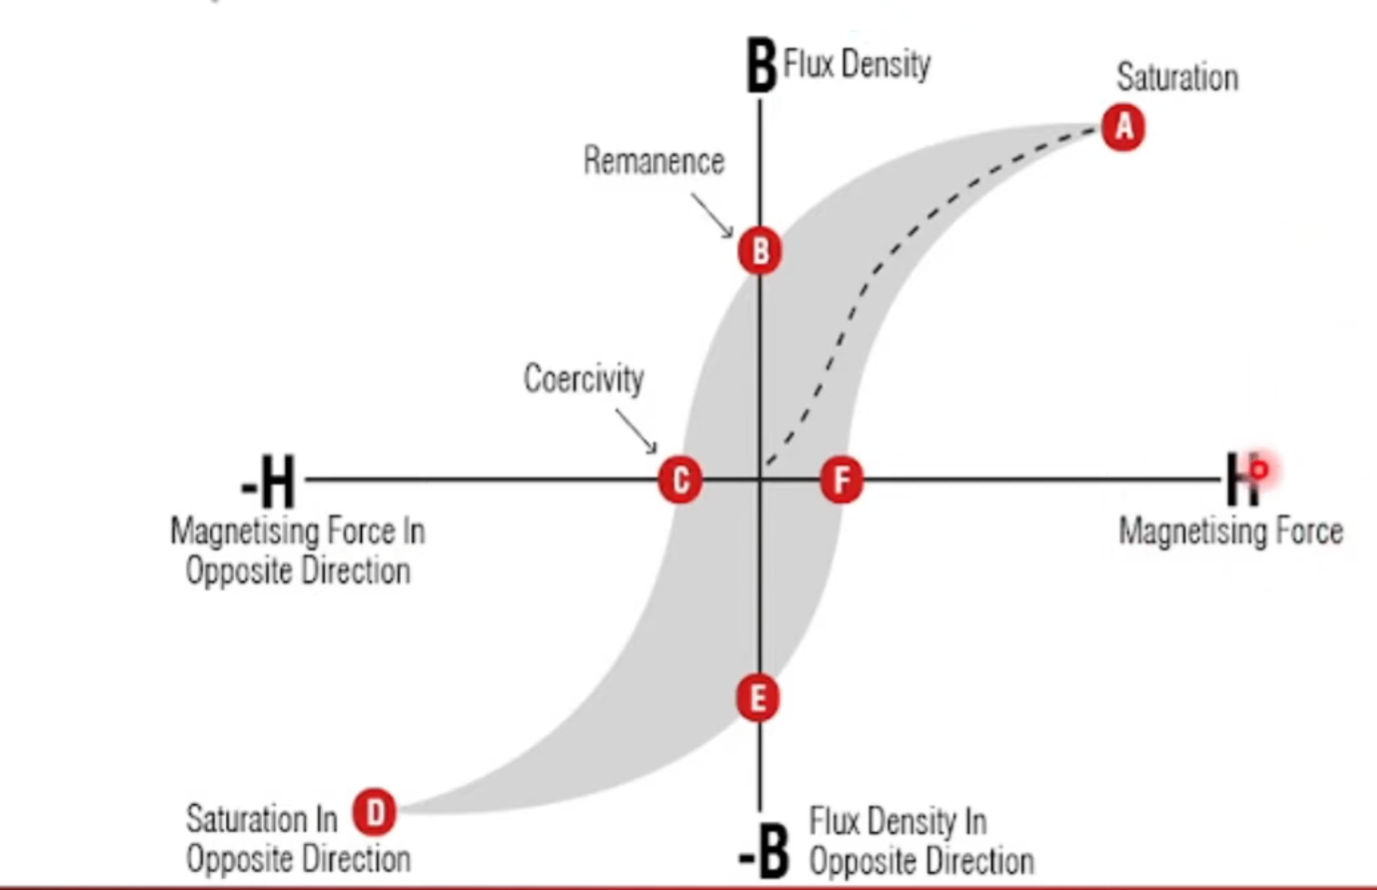
\includegraphics[width=0.85\linewidth]{Images/hysteresis_curve.png}
            \caption{Details of hysteresis curve.}
            \label{fig:hysteresis plot 1 }
        \end{figure}
        \item \underline{Step 1:} When the external field is applied in the $\mathrm{+ve}$ H direction, the spins/magnetic moment tries to align in the direction of the applied field. 
        \item \underline{Step 2:} Now if the external magnetic field is reduced, there remains some magnetization in the system. It does not trace back the same path and at 0 external field the magnetization is changed, this is termed as Remanence, and this is called Retentivity of the system.
        \item \underline{Step 3:} Further, to reduce the magnetization to its initial state, a negative external field is applied and at specific value the magnetization is reset and that point is termed as " Coercivity" and that field is called as coercive field.
        \item \underline{Step 4:} Again, when the magnetization is increased continuously in the negative direction, the magnetic moments/spin will orient in that direction and reaches saturation in the negative direction. 
    \end{enumerate}
    \item Spontaneous Magnetization disappears at $\mathrm{T_c}$ (\textbf{Ferromagnetic transition/Curie Temperature})
    \item Well above the transition temperature, material behaves like the paramagnetic material which is given by the Curie-Weiss Law,
    \begin{equation}
        \mathrm{T_c},\chi=\frac{C}{T-T_c}
        \label{eqn: curie-weiss law}
    \end{equation}
    \item Above $\mathrm{T_c}$ the magnetic moments are oriented randomly with net zero magnetization which is only in the case of paramagnetic materials.
    \item Made of large number of domains and each domain contains about $(10^9-10^{15})$. The direction might be different in different domains, but the direction in a particular domain would be the same. And the magnitude of the magnetic moment in the single domain is determined by the vector sum of the individual domains, schematically represented in figure \ref{fig:magnetic domains example}. And the boundaries which separates them is called \hl{domain-walls}. 
    \begin{figure}[h!]
        \centering
        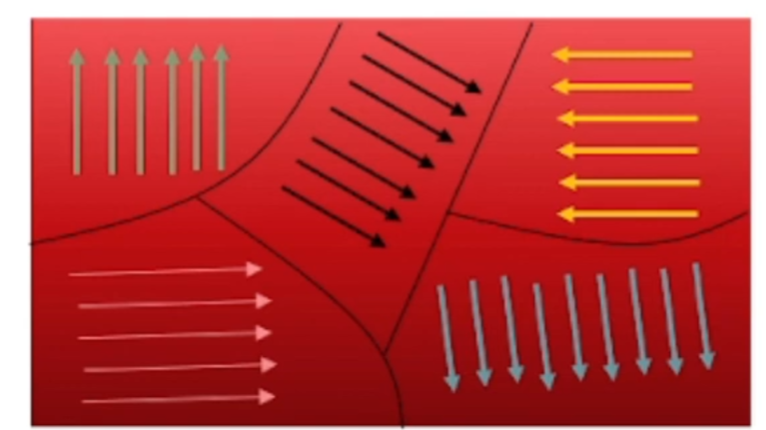
\includegraphics[width=0.75\linewidth]{Images/domains_example.png}
        \caption{A schematic representation of the magnetic domains in a ferromagnetic material.}
        \label{fig:magnetic domains example}
    \end{figure}
    \item Saturation magnetization (spontaneous magnetization in the case of temperature less than $T_c$) is increasing as the temperature decreases and maximum at $\mathrm{T=0} K$. This is also known as the normalized magnetization.
    \item Generally ferromagnetism appears in both metals and insulators.
\end{enumerate}
% \subsection*{V2. Weiss Molecular Field Theory|Exchange Field Theory|Curie Weiss Law}
\addcontentsline{toc}{subsection}{2. Weiss Molecular Field Theory|Exchange Field Theory|Curie Weiss Law}

This video is more about the introduction to Weiss Molecular Field Theory.
\begin{enumerate}
    \item In 1907, in order to explain spontaneous magnetization Weiss assumed that there exists an exchange field acting on a dipole which is given by:\\
    \begin{equation}
    \begin{split}
    H_{\mathrm{ex}} &= H_a + H_w \\
    H_{\mathrm{ex}} &= H + \lambda M
    \end{split}
    \end{equation}
    where $\mathrm{H_a}$ is the applied field, and $\mathrm{H_w}$ is the weiss field, and $\lambda$ is the Weiss constant.
    \item The Weiss field is proportional to its magnetization.
    \item Weiss constant determines the strength of the interaction of between the magnetic dipole moment in a material.
    \item In ferromagnetism, Curie law holds for exchange field as well.
\begin{figure}[htbp]
\centering
\begin{minipage}{0.55\textwidth}
\begin{equation}
\begin{split}
\chi &= \frac{C}{T} \\
\frac{M}{H_{\mathrm{ex}}} &= \frac{C}{T} \\
\frac{M}{H + \lambda M} &= \frac{C}{T} \\
M(T - \lambda C) &= C H \\
M &= \frac{C H}{T - C\lambda} \\
\chi &= \frac{C}{T - C\lambda}
\end{split}
\end{equation}

\vspace{0.5em}

\begin{equation}
\boxed{
\chi = \frac{C}{T - T_c}
}
\end{equation}
\end{minipage}
\hfill
\begin{minipage}{0.4\textwidth}
\centering
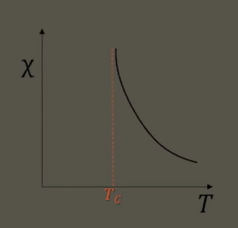
\includegraphics[width=\linewidth]{Images/Curie-weiss law.png}
\caption{Schematic graph of the Curie--Weiss law.}
\label{fig:curie-weiss-law}
\end{minipage}
\end{figure}
    \item This condition is only applicable above the transition temperature and this law is called as \hl{Curie-Weiss Law}.
    \item \textbf{Cases}:
    \begin{itemize}
        \item As $T\to T_c$, $\chi\to \infty$
        \item For $T<T_c$, Spontaneous magnetization exists, which means below the $T_c$ the material is acting as the ferromagnetic materials.
    \end{itemize}
    \item Temperature Dependence of Spontaneous Magnetization:
    \begin{itemize}
        \item Consider a spin system below $T_c$
        \item When $H=0$, \begin{equation}
            H_{ex}=\lambda M
        \end{equation}
        where $M=N\bar{\mu}$
    \end{itemize}
    \item According to quantum theory of paramagnetism, magnetization for spin half is;
\begin{figure}[htbp]
% \centering
\begin{minipage}{0.35\textwidth}
\begin{equation}
\begin{split}
M &= Ng\mu_B \tanh(x) \\
\mathrm{where}, g=1+\frac{J(J+1)+S(S+1)-L(L+1)}{2J(J+1)} \\
\mathrm{x}&= \frac{\mu_BgB}{\mathrm{k}T} \\
\end{split}
\end{equation}

\vspace{0pt}
\end{minipage}
\hfill
\begin{minipage}{0.3\textwidth}
\centering
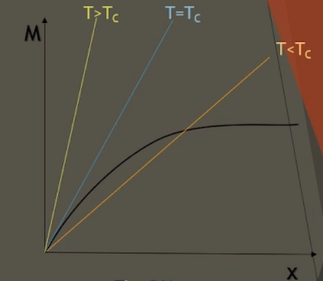
\includegraphics[width=\linewidth]{Images/temp_dependence.png}
\caption{Schematic graph of the temperature dependence of Curie-Weiss law.}
\label{fig:temperature dependence}
\end{minipage}
\end{figure}
\item In the case of ferromagnets we will have the nature of the plot as the $y=mx$ type plot. Only the different temperature will have different straight lines. $M=\left(\frac{kT}{\mu_0\mu_Bg\lambda}\right)x$. This is the final equation in the case of ferromagnets. 
\item As $T\uparrow,$ slope of straight line $\uparrow$.
\item For $T<T_c,$ two curves intersect which gives spontaneous magnetization. [\textcolor{red}{Q.When is the spontaneous magnetization is going to be maximum?}]
\item Maximum spontaneous magnetization occurs at $T=0$ K.
\item At $T=T_c,$ straight line is tangential to hyperbolic curve at origin.
\item For $T>T_c,$ spontaneous magnetization remains zero.
\item For normalized magnetization, the thermomagnetic equation of the state for ferromagnetic phase, is given by;
\begin{equation}
 \begin{split}
   \frac{Ms(T)}{M_s(0)}=\frac{Ng\mu_B \tanh{(T/T_c)}}{Ng\mu_b}\\
   \frac{Ms(T)}{M_s(0)}=\tanh{(T/T_c)}
 \end{split}    
\end{equation}
\end{enumerate}
% % \subsection*{V3. Heisenberg Exchange Interaction|Relation between Exchange integral and Weiss Constant}
\addcontentsline{toc}{subsection}{3.  Heisenberg Exchange Interaction|Relation between Exchange integral and Weiss Constant}
\label{chap:Magnetism/Heisenberg_Exchange}

\subsection*{Jan 15, 2026}
This video is about the Heisenberg Interaction which will tell us the limitations of the Weiss molecular field theory

I have made the notes in the Good Notes. I should re type it here and have done the notes till the time stamp of 8:30 only for this video. Need to complete watch and then remake the note and watch it tomorrow.


% % \subsection*{V9. Spin waves|Magnons|Dispersion Relation for Spin wave}
\addcontentsline{toc}{subsection}{9. Spin waves|Magnons|Dispersion Relation for Spin waves}
\begin{enumerate}
    \item Analogous to lattice waves.
    \item Generated due to the exchange forces.
    \item \hl{Collective motion of magnetic moment in magnetically ordered materials like ferromagnetic materials}.
    \item Due to some external disturbance, these magnetic moment goes to some motion which give rise to spin-waves.
    \item Can be also called as the wave of a quantized energy that propagates through a substance as a result of magnetic field shifts within an atom in response to an outside stimulus (alternating field).
    \item Quantization of spin waves gives us \hl{\textbf{Magnons}}.
    \item \textbf{Magnons:} 
    \begin{enumerate}[(i.)]
        \item Collective excitations of electrons' spin structures in a crystal lattice, crystal should be magnetic in nature, where the order state is observed, i.e., ferromagnetic or antiferromagnetic and also ferrimagnetic substances.
        \item Magnons are a quasi particle.
        \item Quasi particle means the particle which can only exists when interaction is taking place, that means inside the interacting many particle systems.
        \item They are Bosons and obeys Bose-Einstein theory.
        \item Spin = 1 (integral spin)
        \item First introduced by Felix Bloch in 1930, used to introduce to explain the reduction of spontaneous magnetization in ferromagnets.
        \item $\mathrm{T=0}$ K, lowest energy state with parallel atomic spins.
        \item As the temperature is increased, there is increase in the internal energy (randomness in the system) of the system, and decrement in the spontaneous magnetization which as a result \textbf{magnon} is created.
        \item Each magnon will reduce total spin by 1 $\mathrm{\hbar}$ and magnetization is reduced by $\mathrm{\gamma\hbar}$, where $\mathrm{\gamma}$ is the gyromagnetic ratio\footnote{Ratio of magnetic moment to the angular momentum.}.
        \item Experimentally detected in 1957 by Bertram Brockhouse by inelastic neutron scattering in ferrite.
        \item Detected in Ferro-, Ferri-, and Anti-ferromagnets.
    \end{enumerate}
    \item Dispersion Relation for Spin waves:
    \begin{enumerate}[(i.)]
        \item Ferromagnetic ground state is ordered one, hence magnon is not created. 
    \end{enumerate}
    \item Quantized lattice waves gives us \hl{\textbf{Phonons}}.     
\end{enumerate}
\subsection*{V6. Origin of Ferromagnetic Domains|Need, Energy terms|Formation \& Shape, Equations with Explanation}
\addcontentsline{toc}{subsection}{6. Origin of Ferromagnetic Domains|Need, Energy terms|Formation \& Shape, Equations with Explanation}

\textcolor{red}{Q.No. 1 Why does iron pieces do not attract each other? why do they need a magnet to attract each other?}\\
\ding{228} This can be explained by the concept of domains.
\begin{enumerate}
    \item Weiss postulated that the ferromagnetic substance is divided into a large number of small domains. In each of these domains, the magnetization is aligned in one direction. The direction of magnetization in each domain are opposite and tends to cancel each other.
    \item Each dimension is magnetized but the directions of magnetism in various domains tends to cancel each other.
    \item The Net magnetization is zero.
    \item \textcolor{red}{\textbf{How to see Domains?}}
    \begin{enumerate}
        \item It was developed by Francis Bitter in 1931.
        \item In this method, the surface of the sample is covered with an aqueous solution of very small colloidal particles of magnetite $\mathrm{(Fe_3O_4)}$.
        \item Magnetite deposits as a band along the domain boundaries, at their intersection with the sample surface.
        \item Outlines of domains can be seen using a microscope.
        \item In general we can see the domains by following steps:
        \begin{enumerate}
            \item Carefully polish the surface of ferromagnet.
            \item Spread a fine powder of ferromagnetic particles over it.
            \item Particles collect over domain boundaries.
            \item Observed using different microscopy methods. Some of them are listed below.
        \end{enumerate}
    \end{enumerate}
    \item \textbf{Visualization of Magnetic Domains:}
    \begin{enumerate}
        \item Images and details of different microscopy like, Kerr Microscope, Magnetic Force Microscopy, and Lorentz Transmission electron microscopy are just said and images are provided in this section.
    \end{enumerate}
    \item \textbf{Formation \& shape of Domains:}
    \begin{enumerate}
        \item The formation and the shape of domains depends on the competition among different energy terms present in the magnetic crystal.
        \item Consider a uniformly magnetized state of a crystal, which means the exchange energy is lowest, and it can be said that this have large amount of magneto-static energy. 
        \item Magneto-static energy is a self energy due to interaction of magnetic field due to magnetization in some part of the sample on the other parts of the same sample.
        \item This energy depends on the volume occupied by magnetic field extending outside the domain.
        \item As in the uniformly magnetized charge which is on the surface of the sample. These charges are going to produce the magnetic field which will be in the opposite direction to that of the magnetization and that field which opposes the magnetization is called the demagnetization field which will be always opposite to $\mathrm{\overrightarrow{M}}$ denoted as $\mathrm{\overrightarrow{B_d}}$.
        \item Hence, we can say that the net magnetization would be the competition between these two fields.
        \item $\mathrm{\overrightarrow{M}}$ is opposite to $\mathrm{\overrightarrow{B_d}}$.
        \item Magneto-static energy is positive.
        \item The corresponding density is given as,
        \begin{align}
            E_m &= \frac{1}{2} M B_d 
            \intertext{where, the demagnetizing field is given by,}
            \vec{B}_d &= -\mu_0 D \vec{M}
        \end{align}
         where, $D$ is the demagnetization factor and is large for flat sample and small for elongated sample.
        and demagnetization energy is given as
        \item We can see that the demagnetization field is itself dependent on the the magnetization and it comes into the picture only when there is surface magnetic charges present in the system.
        \item 
    \end{enumerate}
    \item  
\end{enumerate}
% \chapter{Research Papers}
\label{chap:research-papers}

\underline{\textbf{Objective question for Research:-}}

% This explanation is for the PSSW related papers.
% \large{Does a static magnetic field contribute to the excitation of perpendicular standing spin-wave (PSSW) modes, and can this contribution be identified from the results of this work?}

% This explanation is related to the Exchange bias based papers.
Look for exchange bias in the $\mathrm{CoFe/FeO}$ bilayer, then try changing the interface damping and the anisotropy value, and varying the thicknesses of the ferromagnetic (FM) and antiferromagnetic (AFM) layers.


\section{FMR studies of surface and bulk spin-wave modes in a CoFe/PtMn/CoFe multilayer film - \href{http://dx.doi.org/10.1063/1.2839337}{JAP 103, 07B525 (2008)}}
\subsection*{Main points from the Paper}
\begin{enumerate}
    \item Studied the exchange-dominated surface and bulk spin-wave modes in a single period of CoFe/PtMn/CoFe trilayer film.
    \item Multimode spin-wave spectra was observed using the FMR. Also, they have identified a high-order standing spin wave in the spectra and found \textbf{"critical angle"} in the multilayer sample. They have also included the effective surface anisotropy field to describe the results.
    \item They have used FMR to investigate the exchange-dominated surface and bulk spin-wave modes in a single period of CoFe/PtMn/CoFe tri-layer film. Bulk magnetic anisotropy parameters and the g-factor of the magnetic film based on the angle dependence of the main resonance field.
    \item A significant enhancement in the in-plane anisotropy was observed in the range; $\sim57-123$ Oe.
    \item A high-order standin spin wave was identified in our spectra along with a "critical angle" in the trilayer sample. 
    \item An effective surface anisotropy field due to the exchange bias and the dynamic surface spin pinning was also used to describe the results.
    \item The exchange interaction stiffness in the CoFe layers, $J\sim 2.7$ meV.
    \item \underline{Acoustic spin-wave mode:} The acoustic spin wave mode is the lowest-frequency mode where all spins in the material move together and stay in phase across the thickness. e.g. In a thin ferromagnetic film, all magnetic moments tilt and precess together when a microwave field is applied.
    \item \underline{Higher-order standing SW:} Higher-order standing spin wave modes occur when spins form standing patterns across the thickness, with some regions moving opposite to others. e.g. In a thick magnetic film, the magnetization oscillates with one or more nodes across the thickness, similar to standing waves on a stretched string.
    \item These results could be related to the change of surface spin pinning is also said in the paper.
    \item A two-fold symmetry for the out-of-plane geometry is observed when the angular dependence of the resonance filed of the acoustic spin-wave mode is measured.
    \item The excitation of the spin-wave precession is due to the absorption of microwave. 
    \item The effective parameter A changes with changing angles when we rotate the sample, and the magnetic profile changes due to the change of the surface pinning. This results in the change of the spin-wave resonance energy.    
\end{enumerate}
\subsection*{Summary}
In summary, we investigated the basic magnetic excitations in a CoFe/PtMn/CoFe multilayer film using the FMR technique. A higher-order spin-wave mode appears only after the magnetic field is tilted beyond a certain angle. By considering an effective surface anisotropy field, the observed spin-wave resonance spectra can be explained by dynamic pinning of spins at the surfaces.


 %2008 PSSW paper
\section{Perpendicular standing spin wave and magnetic anisotropic study on amorphous FeTaC films - \href{https://doi.org/10.1109/TMAG.2016.2520981}{TMAG 7 52, 2520981 (2016)}}

\begin{description}
    \item[\underline{Perpendicular Standing spin-wave (PSSW):}]A perpendicular standing spin-wave is a magnetic excitation in a thin film where the spins oscillate in a standing-wave pattern across the film thickness, that is, perpendicular to the film surface.

    E.g: In a thick ferromagnetic film measured by FMR, higher-order resonance peaks appear because the magnetization forms standing waves between the two film surfaces.
\end{description}
\subsection*{Main points from the Paper}
\begin{enumerate}
    \item Magnetic anisotropy, spin wave (SW) excitation, and exchange stiffness constant of amorphous $\mathrm{Fe_{80}Ta_8C_{12}}$ $(d=20 - 200 \mathrm{nm})$ films were studied as a function of thickness using microstrip-FMR.
    \item The amorphous nature of the soft ferromagnetic (FM) alloys has no grain boundaries, which is important for the magnetization reversal and enhances the speed of spin-switching in spin transfer torque devices.
    \item In the case of FMR, the external microwave field couples with uniform and nonuniform SW modes. This excitation of magnetistatic modes occurs especially in dipole-dipole interaction dominated system where the wave vector $(\vec{q})$ lies in the plane.
    \item The modes with wave vector $(\vec{q})$ component perpendicular to the film surface is termed perpendicular standing spin-wave (PSSW) modes and the quantization of these modes is due to the geometrical confinement \cite{gui2007quantized}. 
    \item According to the Kittel model, the excitation of odd SW modes can be observed with the spin pinned by surface anisotropy interaction. However, in the case of partially surface pinned spins, both even and odd SW modes can be excited.
    \item The magnetic field sweep FMR spectra were carried out for different precessional frequencies and azimuthal angles.
    \item By increasing the thickness of the film $(\geq100 \mathrm{nm})$, $M-H$ curve clearly shows the transcritical loop manifesting the presence of stress-induced perpendicular anisotropy during the film deposition.
    \item The room temperature soft magnetic properties degrade drastically as the thickness increases due to the transition from the in-plane orientation of magnetization to the strip domain patterns.
    \item At the thickness of 20 nm a clear uniform precession mode without any other SWR mode in which the dynamic magnetization is uniform across thickness. 
    \item However, when the thickness is increased from 50 nm onward, the first PSSW mode is excited at lower absorption fields. The signal strength is 7 times smaller than the uniform mode.
    \item The absence of the higher order $(n>1)$ exchange-dominated PSSW modes could be due to very weak excitation, and the intensity of those nodes may be lower than our detection sensitivity.
    \item The increasing differences between the first PSSW modes and the uniform mode, could be understood on the basis of perpendicularly quantized SW vector, which is inversely proportional to the film thickness, i.e., $q=n\pi/d$.
    \item The angular dependence of resonance fields is governed by uniaxial magnetic anisotropy, in the case of 20 nm, $\phi_H$ dependence of $H_r$ for uniform mode at 6, 8 , and 10 GHz precessional frequencies.
    \item The typical field dependence of the resonant frequencies are shown in fig: 3(b). \hl{Watch this in detail}.
    \item The origin of in-plane uniaxial magnetic anisotropy in FeTaC thin films $(d=20$ and $50$ nm$)$ could be understood on the basis that the strong exchange coupling between the FM atoms plays an important role during the deposition process, which allows to form aligned FM atom pairs parallel to the film plane. 
    \item On further increase of the thickness, the in-plane uniaxial magnetic anisotropy disappears. 
\end{enumerate}
\subsection*{Summary}
The MS-FMR method was used to study magnetic anisotropy and spin-wave excitations in soft ferromagnetic FeTaC films. The angular variation of the resonance field within the film plane indicates a weak uniaxial anisotropy for films with thicknesses of 20 and 50 nm. Along with the uniform precession mode, the observation of the first perpendicular standing spin-wave mode confirms the role of both exchange and dipolar interactions. The exchange stiffness constant of these amorphous films was obtained from the in-plane angular behavior and from the frequency separation of the PSSW mode measured along the easy and hard magnetization directions. The extracted exchange stiffness increases from $2(4)\times10^{-7} \mathrm{to} 3.5(5)\times10^{-7}$ erg/cm as the film thickness increases from 50 to 200 nm. % 2016 ANjan Barman PSSW paper
\section{Perpendicular standing spin waves in AuPt/GdFeCo induced by spin-orbit torques - \href{https://doi.org/10.1038/s42005-025-02433-2}{Comm. Phys.,8, 516 (2025)-Nature}}

\section*{Main points from the Paper}
\subsection*{\underline{I. Introduction:}}
    \begin{enumerate}[1.]
        \item GdFeCo has a ferrimagnetic compositions, their spin dynamics in the present regime are effectively ferromagnetic (FM).
        \item They have observed the SOT, generated from the adjacent AuPt layer induce perpendicular standing spin waves in GdFeCo, with resonant modes observed up to the third order. 
        \item Uncapped films exhibit oxidation-induced degradation that suppresses spin-wave confinement and to avoid that they have used Ta as the capping layer. 
        \item Ferrimagnetic materials (FiMs) can also be used to provide most of the things which are useful in device chips which require a faster switching speeds and reduced saturation magnetization [\textcolor{red}{first lines are good}].
        \item The combined properties of FM and AFM are found in the FiMs: low net saturation magnetization, fast magnetic dynamics driven by antiferromagnetic precession, and the ease of magnetization manipulation and detection typically seen in ferromagnets.
        \item Because of the presence of the forced precession of antiparallel spins in FiMs, there is formation of perpendicular standing spin-waves(PSSW) modes, where spins oscillate perpendicular to the film surface.
        \item The formation of PSSW modes was observed recently in AFM or FiM systems in connection with FM which is attributed to the interlayer exchange coupling with the adjacent FM layer. 
        \item ST-FMR is used to observe the PSSW modes in AuPt/GdFeCo.
        \item In the case of uniform precession of the magnetic moments $(p=0)$ or PSSW modes when spin waves witht non-zero wave vectors satisfy the confinement condition \boxed{$(k=p\pi/d)$} where $d$ is the film thickness.
        \item The Ta capping layer was used as capping layer to reduce the oxidation and enabled us to stabilize the PSSW modes up to the $p=3$. And the samples without the Ta capping, the ST-FMR spectra with PSSW modes were limited to the $p=2$ and a reduced saturation magnetization compared to those with the Ta capping layer.
        \item These findings provide valuable insights for the development of FiM-based SOT-MRAM and logic devices, which benefit from the unique properties of FiMs.
    \end{enumerate}
\subsection*{\underline{II. Results and Discussion:}}
\begin{enumerate}[1.]
    \item VSM is used to measure the fundamental magnetic properties of the system, and saturation magnetization $(M_s)$ and effective anisotropy energy density $(K_{eff})$ as a function of GdFeCo thickness is calculated. \footnote{See the supplementary note 1 of the paper for detailed calculations of these.}
    \item Surface effects was taken as the reason why there is larger saturation magnetization $(M_s)$. On increasing thickness, the bulk properties becomes more dominant enhancing ferrimagnetic ordering and a reduction of overall magnetization.
    \item Suppression of oxidation significantly affects the magnetization, particularly at lower thicknesses.[\textcolor{red}{Important Line}]
    \item Surface anisotropy weakens as $t_{GdFeCo}$ increases, leading to bulk anisotropy becoming dominant contribution. It is consisted with $M_s$ results.
    \item No PMA has been observed across the entire thickness range.
    \item The spin currents generated by the Spin Hall Effect (SHE) from the strong SOC in the adjacent AuPt layer and the induced $H_{Oe}$ produced by the RF current drives the magnetization dynamics in the GdFeCo layer, where the antiparallel alignment of magnetic moments results in varying precession amplitudes and directions among individual atoms.
    \item The excited spin-wave modes generated by this dynamic behavior exhibit the PSSW modes when teh wave vectors $(k)$ satisfy the confinement condition, $k=p\pi/t_{GdFeco}$.
    \item The Ta layer prevents the formation of FeO, CoO, or GdO hence the 3rd mode $(p=3)$ is only present in the case of Ta capping.
    \item Experimental evidence of presence of 3rd PSSW mode in the presence of the Ta layer was observed. This enhances the surface pinning and spin-wave reflection, promoting the formation of higher-order PSSW modes.
    \item The sharp increase in $(A_{ex})$ at $t_{GdFeCo}=80$ nm is attributed to the dominant bulk properties in the GdFeCo layer. This irregular behavior suggests that spin-wave propagation and PSSW formation are hindered by spin-wave absorption and reduced spin-wave reflection due to surface oxidation.
    \item The interfacial engineering after adding Ta as the capping layer, stabilizes the ferrimagnetic dynamics, promoting the formation of higher-order spin-wave modes.
    \item The dynamic pinning model and introduced the wave vector$k_p$ defined as $k_p=\left[\frac{(p+\delta)\pi}{t_{GdFeCo}}=\frac{2\pi}{\lambda_p}\right]$, where $\lambda_p$ is the wavelength in the GdFeCo layer, accounting for each mode  $p$ and the pinning parameter $\delta$ was used by the authors to quantify the degree of pinning at the surface. [\textcolor{red}{ref. 49-51, from this paper}].
    \item When the Ta capping was done on the system here, this pinning model specified that there is strong interfacial confinement and in the case of not Ta capping, there was significantly lower confinement.
    \item Conclusively, the Ta capping enhances the interfacial confinement, supporting the formation of stable and higher-order PSSW modes.
    \item When magnetic field polarity measurements were carried out, the 1st PSSW mode was only visible under a positive external magnetic field. In contrast, the Ta-capped samples exhibit symmetrical resonance under both positive and negative external fields. 
    \item The oxidation of the Gd leads to the asymmetrically aligned local magnetic moments, breaking the mirror symmetry with respect to the external magnetic field.
    \item Potential mechanisms may include non-reciprocal spin-wave propagation in magnetization-graded systems or the influence of the Dzyaloshinskii-Moriya interaction (DMI) [\textcolor{red}{ref. 56-59 from this paper}]. 
\end{enumerate}
\subsection*{\underline{III. Summary:}}
\begin{enumerate}
    \item An investigation of the formation of PSSW modes in ferrimagnetic GdFeCo layers drive by SOTs generated by the adjacent high SOC material, AuPt was carried out.
    \item The ST-FMR spectra explains the induced antiparallel magnetization precession after the contact of AuPt which injected the SOT.
    \item Oxidation at the surface of GdFeCo was shown to significantly affect the key properties such as $M_s,A_{ex}$, and overall quality of deposited GdFeCo layer.
    \item The pinning effects at the interfaces were evaluated using a dynamic pinning model, demonstrating that the Ta-capped samples provided strong interfacial confinement for PSSW modes, while the uncapped samples exhibited relaxed boundary conditions and weaker pinning.
\end{enumerate}
 % 2025 Very recent PSSW paper AuPt/GdFeCos
\section{Perpendicular standing spin waves in films with interfacial Dzyaloshinskii-Moriya interaction - \href{https://doi.org/10.1103/PhysRevB.111.064432}{PRB, 111, 064432 (2025)}}

\section*{Main points from the Paper}
\subsection*{\underline{I. Introduction:}}
\begin{enumerate}
    \item As Dzyaloshinski Moriya interaction (DMI) is known to induce the nonreciprocity in spin wave propagation within the plane of magnetic thin films.
    \item Analytical expressions are developed to estimated the effecets of DMI on spin waves by assuming the magnetization dynamics are uniform throughout a film thickness.
    \item The calculations done here show that the PSSW mode frequencies depend nonlinearly on the interfacial DMI strength and on the inverse thicknesses of the magnetic films.
    \item DMI is an antisymmetric exchange interaction caused by spin-orbit coupling and broken symmetry that enforces a preferred rotational sense in magnetic textures and their stabilization. It exists when the following conditions are met:
    \begin{enumerate}[\ding{212}]
        \item Strong spin-orbit coupling (usually from heavy metal).
        \item Broken inversion symmetry (typically at an interface).
    \end{enumerate}
    \item Generally Spin waves are the fundamental excitations of magnetic materials. 
    \item Spin waves in thin films are affected by interfacial DMI, leading to exciting phenomena such as nonreciprocal propagation, spin wave focusing, and even the loss of standing wave modes[\textcolor{red}{ref. 17-19}].
    \item Spin waves do provide the tool to measure the DMI experimentally \cite{stashkevich2015experimental,nembach2015linear}.
    \item Usually, in the theoretical studies of spin waves affected by DMI have assumed that the magnetization is uniform through the magnetic film's thickness \cite{moon2013spin,cortes2013influence}.
    \item The atomic layer method has been used to treat antiferromagnetically coupled stacks of thin films, exchange spring bilayers, and thin films with magnetoelectric coupling at interfaces \cite{moore2014spin}.
\end{enumerate}
\subsection*{\underline{II. Results and Discussion:}}
\subsubsection*{\centering A. One FM material}
\begin{enumerate}
    \item In the case of single FM material, it is assumed that the magnetization precession is uniform through the film.
    \item The full dipolar contribution is also included in the dispersion relation in Ref. \cite{moon2013spin}.
    \item The interfacial atomic DMI constant $D_{at}=4.2$ mJ$/m^2$ acts at the top layer only, which corresponds to an effective DMI used in the analytic expression of $D_{\mathrm{eff}}=D_{\mathrm{at}}/N=1.05$ mJ$/m^2$.
    \item The presence of DMI results in a pinning of a PSSW modes at the top surface, which is undetectable. The pinning is different for spin waves depending on the sign of $k_x$.
    \item One can see that without DMI, the mode is truly uniform through the film thickness, but with DMI and depending on the sign of $k_x$, the pinning results in nonuniform precession.
    \item Higher order standing spin waves are extremely sensitive to DMI because their motion is strongly confined across the film thickness, causing DMI and exchange to interact in a complex, non-additive way.
    \item It is well studied that increasing the thickness $L$ of a film will decrease the exchange energy and will therefore decrease the frequencies of higher-ordered PSSW [\textcolor{red}{ref. 36 \& 37}].
    \item The interface modifies the mode which then modifies the exchange interactions. And as a result, the frequency and damping is also modified. In our case this explains the non-monotonic damping trends.
    \item \hl{The system transitions from uniform-mode dynamics to exchange-dominated multi mode dynamics with increasing thickness}.
\end{enumerate}
\subsubsection*{\centering B. Two FM material}
\begin{enumerate}
    \item Interface position matters more than the interface strength. MgO interface is on one side only which introduces the asymmetry. Boundary conditions produce mode reshaping similar to FM bilayers.
    \item MgO in the case of my system can modify the local exchange interactions, orbital hybridization, and magnetoelastic coupling. Hence, the system behaves like a soft-hard exchange bilayer, even if chemically single phase. This justifies clearly the thickness dependent PSSW appearance in my work. [\textcolor{red}{V. Imp Line}]
    \item Thin films \ding{213} interface dominates \ding{213} uniform mode only.
    \item Thick films \ding{213} exchange resolved \ding{213} asymmetric standing modes appear.
    \item Novelty can be claimed on following points;
    \begin{enumerate}[\ding{212}]
        \item Mode-dependent damping
        \item Thickness-dependent transition from uniform to exchange-dominated dynamics.
        \item Interface-controlled PSSW emergence without explicit DMI.
    \end{enumerate}
\end{enumerate}
\begin{physicsmodule}{Related to my Paper}{Brown}
  \begin{lawbox}
    \subsection*{\sffamily\bfseries CoFe/MgO}
    \ding{212} In thicker CoFe films, perpendicular standing spin-wave modes emerge due to enhanced exchange confinement across the film thickness. These higher-order modes exhibit strong sensitivity to interfacial effects arising from the CoFe/MgO interface. Although such interfacial contributions are localized, they modify the standing-wave profile, leading to a nonlinear coupling between exchange-dominated dynamics and interface-induced fields. As a result, higher-order PSSW frequencies and damping respond more strongly than the uniform mode, consistent with the emergence of mode-dependent dynamic behavior at larger thicknesses.

    \ding{212} For CoFe/MgO, MgO modifies the exchange near the interface, and local anisotropy. This directly affects PSSW formation and damping.

    \ding{212} Studies of multilayer ferromagnetic systems have shown that perpendicular standing spin-wave modes become strongly asymmetric when magnetic properties vary across the film thickness. In such cases, interfacial effects modify the standing-wave profile rather than contributing as simple additive fields, leading to a nonlinear coupling between exchange-dominated dynamics and interface-localized interactions. As a result, higher-order PSSW modes exhibit enhanced sensitivity to interfacial asymmetry, making them effective probes of exchange nonuniformity and boundary conditions. Similar considerations apply to single-layer systems with asymmetric interfaces, where the emergence of higher-order modes reflects a transition from uniform-mode to exchange-resolved dynamics with increasing thickness.
  \end{lawbox}
\end{physicsmodule}
% \subsection*{\underline{III. Conclusion:}} % 2025 Very recent PSSW paper related to DMI
\section{Standing spin waves in Permalloy-NiO bilayers as a probe of the interfacial exchange coupling \href{https://doi.org/10.1103/PhysRevApplied.21.064044}{[\textit{Phys. Rev. Appl., 21 064044 (2024)}]}}

\subsection*{\underline{Abstract}}
The importance of ferromagnetic-antiferromagnetic (FM-AFM) bilayer dynamics, with emphasis on the interaction occurring at the interface, where the magnetic moments of the AFM can be imprinted into the FM, and the exchange bias field can affect these dynamics, is explained in this paper. Here, in this paper, they have used Permalloy (Py) and NiO (Py/NiO) hybrids, and for comparison, single Py films in the broad Py thickness range varied from a few nm to 200 nm by using static (Kerr effect) and dynamic (spin-wave) measurements along with micromagnetic simulations. Uniform precession and perpendicular standing spin waves (PSSWs, $n=1, 2)$ and a clear enhancement of the PSSW mode frequencies upon interfacing Py with NiO, both from experiments and simulations.

\hspace{1cm}The enhancement of the mode frequencies with increasing the thickness of the material, which explains its interfacial origin rooted in the exchange coupling between the FM and AFM layers. \hl{Their results suggest that PSSW detection in a ferromagnet offers a means of probing the interfacial exchange coupling with the adjacent AFM layer}. Furthermore, the controlled spatial symmetry breaking by the AFM layer enables engineering of PSSWs with different spatial profiles in the FM.

\subsection*{\underline{Introduction}}
\begin{enumerate}
    \item The focus on the investigation of ferromagnet-antiferromagnet (FM-AFM) bilayers has been concerned with the induction of uniaxial anisotropy, and recently, a thin FM layer coupled with a thick AFM layer was also studied to observe the AFM spintronics. An important factor present in both of them is the exchange coupling at the AFM-FM interface, since it's not only the shifts that we get in the static hysteresis curves, but it may also affect magnetization dynamics.
    \item Excitation of spin waves (SWs) in a FM coupled to AFM was proposed method to propagate spin excitation into the AFM \cite{jenkinsSpinWaveExcitations2020}.
    \item Recently, PSSWs have been studied in other symmetry-breaking systems like heavy metals-magnetic insulator (HM-MI) bilayers, where the frequency of the standing-wave modes experiences a shift \cite{lee2023erratum}. The effect was attributed to an additional confinement of the waves upon a local increase of the interfacial damping due to spin pumping \cite{lee2023erratum}.
    \item There are other experiments also, as per this paper, which have used PSSWs to probe coupling in FM bilayer or individual surface anisotropies on epitaxial FM layers with nonequivalent interfaces [\textcolor{red}{ref. 10-13,14}]. 

\hl{The introduction part is written in a perfect way. Please read it and get the references. Try to get the exchange length of the CoFe (B2-CsCl structure).}


    \item Lower $M_s$ is set near the top surface of our films. This translates to a lower demagnetizing field and a higher effective potential in these layers, thus enabling the pinning of the PSSW mode. [\textcolor{red}{ref. 30}].
    \item This effect might also be due to the surface oxidation typically experienced by ferromagnetic films or a magnetization symmetry breaking in the normal direction due to a capping layer.
    \item In the case of Py, the variation in the $M_s$ is the most conceivable way to induce changes in the surface pinning parameter \cite{waring2023exchange}, therefore generating magnetization symmetry breaking and allowing the excitation of PSSWs.
    \item The averaged out-of-plane (OOP) magnetization of the system was converted into the frequency domain after the use of a Fourier transform \cite{park2003imaging}. This process was repeated for each of the presented magnetic fields.
\end{enumerate}

\subsection*{\underline{Experimental Results \& Discussion}}
\begin{enumerate}[A.]
    \item \underline{Static Characterization of the Py and Py/NiO films:}
    \begin{enumerate}[1.]
        \item Static MOKE reveals the clear enhancement of the ferromagnetic films upon the addition of NiO. As expected, there is an exchange bias in the FM/AFM layer.
        \item Experimentally, it has been proved that this phenomenon will suppress once the thickness of the FM layer becomes large enough, which can be attributed to the reduced effect of the interface exchange coupling strength relative to the overall magnetization of the film.
        \item They have also observed the shift in the hysteresis loops from a field-centered position, which clearly indicates the presence of an exchange bias field in Py/NiO.
        \item There is also a reduction in the exchange bias field as the Py layer becomes thicker, once again, an effect related to the reduced influence on the overall film magnetization. \hl{Quantifiable exchange coupling within our AFM-FM films}
    \end{enumerate}
    \item \underline{Effect of NiO on the frequency of the observed standing waves}
    \begin{enumerate}[1.]
        \item After doing the VNA-FMR, they have observed a uniform FMR mode, characteristic of the FM layers in the case of both Py and Py/NiO.
        \item The spin-wave modes are identified as exchange-dominated thickness-dependent modes related to PSSWs in our films \cite{dabrowski2021canted}.
        \item The existence of different PSSW modes with the thickness of the films is also observed. 
        \item In this system, the PSSW modes were shifted to higher frequencies, replacing the standing spin-wave modes. The frequency shift decreases with the enhancement of the thickness of the Py layer.
        \item This suggests that there is a direct relation between the magnitude of the magnetic moments in the film as the FM layer grows thicker and the frequency shift of the PSSW modes experienced when the NiO layer is added.
        \item Generally, FMR mode is independent of the thickness; however, in this case, when the thickness is increased, they have observed the frequency shift in the same direction for all of the pairs of samples.
        \item The frequency shift experienced by our films is a direct consequence of the Py magnetic moments pinning at the interface due to the exchange bias. The absence of free spins results in an additional confinement of the PSSWs.
        \item There is the confinement of the PSSW modes when the thickness is reduced to 2 nm, and it is supported by the experiments done on thin films.
        \item The saturation magnetization remained consistent at all thicknesses in the case of Py/NiO.
        \item The anisotropy field progresses similarly to the exchange bias and coercive fields extracted from the static hysteresis loops. This is expected since the exchange bias of the films has less influence on the overall magnetization as the film thickness increases.
        \item There is an increase of Gilbert damping (almost an order of magnitude for smaller Py samples) for Py/NiO. This might be the influence of spin pumping to AFM \cite{wang2020spin} and exchange bias at the interface, freezing the magnetic moments of the Py and preventing larger precessions.
        \begin{figure}[ht]
            \centering
            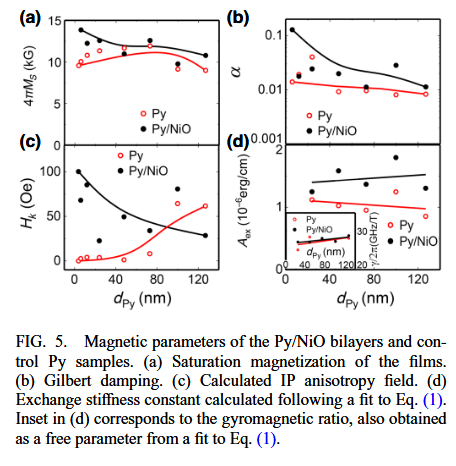
\includegraphics[width=0.65\linewidth]{Images/PSSW_01.png}
            \caption{\textit{Figure from the paper, important one}}
            \label{fig:PSSW_pp1_01}
        \end{figure}
    \end{enumerate}
\end{enumerate}
\subsection*{\underline{Numerical Results of PSSW presence of Py films}}
\begin{enumerate}[1.]
        \item The thickness of the Py films used in the simulation (done by using Mumax$^3$) ranges from 20 nm - 200 nm.
        \item The films are thick enough to accurately resolve the PSSW modes and to observed their possible shifts in the frequency when the interaction with the AFM is introduced.
        \item The surface magnetization gradient caused by a possible oxidation and/or capping, they aim to manipulate the interface pinning parameter, which strongly affects the spin configuration of the PSSW modes across the film \cite{waring2023exchange}.
        \item Not taken in account the surface anisotropies.
        \item Weaker modes above 30 GHz are not observed experimentally in our system due to the strong losses experienced at high frequencies.
        \item In the case of simulation, the detected nodes, $n>0$ are proportional to $1$/$d^2_{Py}$. This agrees with the reports on PSSWs in other FM films.
        \item The frequency of the bulk FMR remains constant when the thickness of the film is increased. Eventually, two modes combine at $d_{Py}< 110$ nm.
\end{enumerate}
\begin{enumerate}[A.]
    \item \underline{Simulating the Py/NiO interface. Optimization of the Uniaxial anisotropy}\\
    The simulations of magnetization dynamics in the AFM-FM bilayer were performed by introducing an extra layer in the system as an uncompensated AFM. This leads to uncompensated spins at the interface, which lead to an exchange bias between FM and AFM.
    \item \underline{Hybrid modes and effect of the interaction with the antiferromagnet}
    \begin{enumerate}[1.]
        \item In both micromagnetics and Atomistic simulations, AFM sublattices are used to model the system \cite{jenkinsAtomisticOriginAthermal2021,jenkinsAtomisticOriginExchange2020}.
        \item Shift in the frequency of the modes, especially in the experimentally observed first-order PSSW $(n=1)$, is also present in all of the performed simulations featuring an AFM-FM interface.
        \item The uniaxial anisotropy at the interface has a direct influence on the frequency of the PSSWs. As given in the diagram, uniaxial anisotropy induced by the AFM leads to higher-frequency modes.
        \item The frequency of the modes can be further enhanced by introducing a local in-plane exchange bias field in the bottom layer of the order of $H_{eb}=1$ kOe. 
    \end{enumerate}
    \item \underline{Conclusion}
    \begin{enumerate}[1.]
        \item They have detected both perpendicular PSSWs spin waves and quasiuniform modes and found that in sufficiently thick Py films both exhibit a clear frequency shift when Py is exchange coupled to NiO.
    \end{enumerate}
\end{enumerate} % 2024 Standing Spin waves in Py/NiO 
% \section{Interfacial Spin Configurations and the Microscopic Origin of Exchange Bias at the IrMn/CoFeB Interface \href{https://doi.org/10.1016/j.fmre.2026.01.003}{[\textit{Fundamental Research, 8 Jan (2026)}]}}

\section*{Main points from the Paper}
\subsection*{\centering\underline{Abstract}}
\hspace{3cm} Exchange bias fields at antiferromagnet/ferromagnet (AFM/FM) interfaces' physical origin remains incompletely understood. While the most of the spins are strongly coupled to the adjacent CoFeB layer, a small fraction remains pinned to the underlying IrMn underlayer. Micromagnetic simulations indicates that an imbalance in the quantity of antiparallel pinned spins contributes to the observed variation in exchange bias.

\subsection*{\centering\underline{I. Introduction}}
\begin{enumerate}
    \item Study of AFM/FM interface has greater impact in the study of spintronics. Exchange bias, being a notably in the AFM/FM structures have a significant in the performance of spintronic devices.
    \item \hl{Exchange bias (EB)} refers to the shift of the magnetization hysteresis loop caused by interfacial coupling between the AFM and FM layers.
    \item EB was generally used to stabilize the magnetization of the pinnned or reference layer in spin-valve structures and MTJs. Moreover, spin-orbit torque (SOT) switching of perpendicular magnetization without an external magnetic field can be realized by introducing an in-plane EB field.
    \item In this work CoFeB/MgO structure provides strong perpendicular magnetic anisotropy and large tunneling magnetoresistance.
    \item Due to the recent development in the electrical control of EB via SOT has been demonstrated, enabling the development of a novel storage prototype known as AFM random-access memory.
    \item Earlier studies  have explained that EB originates from fully uncompensated AFM spins [\textcolor{red}{ref. 39}], planar domain-wall model to reconcile the quantitative discrepancies between theoretical predictions and experimentally measured the EB fields [\textcolor{red}{ref. 40}]. Subsequently, Malozemoff developed the random-field model to account for the influence of interface roughness and defects [\textcolor{red}{ref. 42}].
    \item These established that the coupling between FM spins and pinned AFM  spins is a key microscopic mechanism responsible for the EB field.
    \item Recently, the electrical control of EB via SOT have shown that spin current can partially switch the EB field, this is particularly attributed to the formation of AFM multidomains during manipulation process, suggesting that the orientations of interfacial AFM spins, and their contributions to the exchange bias field, are more complex than previously studied.
    \item X-ray magnetic circular dichroism (XMCD)  is employed as a high-precession technique for probing and analyzing AFM/FM interfaces.
    \item Measurements are taken as;
    \begin{itemize}
        \item XMCD measurements at different temperature is done.
        \item Element-specific XMCD hysteresis loops are measured to determine the orientation of AFM pinned spins in samples annealed under different magnetic fields.
    \end{itemize}
    \item Micromagnetic simulations show that variations in the exchange bias field are primarily governed by the quantitative imbalance between these pinned-spin populations.
\end{enumerate}

\ding{107} \hl{Materials and Methods section is not included in these notes}.
\subsection*{\centering\underline{II. Results and Discussion}}
\begin{enumerate}
    \item The multilayer exhibits perpendicular magnetic anisotropy along with an out-of-plane exchange bias field. They have observed the monotonically increment in the magnitude of the EB with the annealing field and saturates at $\pm1$ T.
    \item 
\end{enumerate} %2026 Paper related to IrMn/CoFeB
% \section{Magnetocrystalline Anisotropy Enables Field-Free Deterministic Switching in $\mathrm{Tm_3Fe_5O_{12}/Pt}$ Bilayers: An Atomistic Spin Dynamics Study - [\href{https://doi.org/10.1021/acsami.5c23180}{\textit{ACS Applied Materials \& Interfaces}, 2026}]}

\section*{Main points from the Paper}
\subsection*{\centering\underline{Abstract}}
\hspace{2cm} Field-free switching of perpendicular magnetization is done in this paper. They have observed that the cubic magnetocrystalline anisotropy (MCA) of TmIG spontaneously breaks mirror symmetry along the out-of-plane direction, giving rise to $\mathrm{3m-}$symmetric torques that enable deterministic switching without external fields. Systematic tuning of current density and pulse width allows control over the switching-mode. They have also done the comparative simulations on $\mathrm{Y_3Fe_5O_{12} (YIG)}$ to confirm that MCA-driven field-free switching is a universal feature of rare-earth iron garnets.

\subsection*{\centering\underline{I. Introduction}}
\begin{enumerate}
    \item Manipulation of perpendicular magnetization by spin-orbit torque (SOT) has recently emerged as the cornerstone for high-density, ultrafast, and energy-efficient spintronic devices.
    \item In the absence of external symmetry breaking, the system relaxes stochastically into up or down states once the current is turned off.
    \item It is usually enforced by an in-plane magnetic field [\textcolor{red}{ref. 1, 2, 6}]
    \item Eliminating the need for external fields requires intrinsic symmetry breaking.
    \item Recently, crystalline symmetry itself has been identified as an intrinsic pathway to deterministic SOT switching, demonstrated low symmetry materials such as $\mathrm{WTe_2, IrO_2, Ni_4W}$ as well as in  noncollinear antiferromagnets and altermagnets.
    \item These systems exploit symmetry-governed spin textures to generate characteristic angular responses in field-free magnetization switching.
    \item Not relying on the structural asymmetry, the effect originates from the intrinsic MCA of TmIG [\textcolor{red}{ref. 34\&35}].
    \item This discovery highlights a fundamentally new mechanism for field-free SOT switching in high-symmetry crystals, relying on intrinsic anisotropy rather than extrinsic structural asymmetry.
    \item They have done the cubic MCA mediated switching across rare-earth iron garnets and done that for both TmIG and YIG.
    \item This work mainly provides the anisotropy-driven spintronic phenomena and establish a symmetry-based design principle for ferrimagnetic memory and terahertz spintronic applications.
\end{enumerate}
%%%%%%%%%%%%%%%%%%%%%%%%%%%%%%%%%%%%%%%%%%%%%%%%%%%%%%%%%%%%%%%%%%%%%
\subsection*{Meeting with Rajnandini about the TmIG, Jan 24, 2026}
We discussed more in details about the TmIG and we both finalized that we need to just go through the paper first and then can later work on designing the material in the VAMPIRE. 

I will work on the understanding of the \verbatiminput{sim:unit-cell-category} part and then only I will work on developing this system.
%%%%%%%%%%%%%%%%%%%%%%%%%%%%%%%%%%%%%%%%%%%%%%%%%%%%%%%%%%%%%%%%%%%%%%%%%
\subsection*{\centering\underline{II. Methods and Materials}}
\begin{enumerate}
    \item $\mathrm{Tm_3Fe5O_{12} (TmIG)}$ is a cubic rare-earth iron garnet  with lattice constant $\sim 12.3$ \r{A} with Fe$^{3+}$ ions occupying octahedral (a-site) and tetrahedral(d-site) positions, while Tm$^{3+}$ ions reside in dodecahedral (c-site) positions.
    \item There is antiferromagnetic coupling between the Fe sublattices and parallel alignment of Tm$^{3+}$ moments with a $a$-site Fe$^{3+}$ sublattice yield a ferrimagnetic ground state with non-zero net magnetization.
    \item Though being TmIG as intrinsic cubical anisotropic, the magneto elastic coupling plays a crucial role in orienting the magnetization in epitaxial TmIG thin films.
    \item Here, they have considered an epitaxial $(111)$-oriented TmIG film capped with a Pt layer.
    \item TmIG being a magnetic insulator, the charge current is limited to the adjacent Pt layer, with TmIG magnetization switching driven by SOT generated from Pt-converted pure spin current injected into TmIG.
    \item The \hl{details of the simulations} are given below:
    \begin{enumerate}[\ding{212}]
        \item The damping parameter used is, $\mathrm{\alpha=0.033}$.
        \item The three-sublattice model $(\mathrm{Fe_1, Fe_2, Tm})$ is used with periodic boundary conditions in the $\mathrm{x-y}$ plane.
        \item The TmIG film is oriented along the $[111]$ axis normal to the plane.
        \item The Hamiltonian only includes the exchange interactions, uniaxial PMA, and MCA terms. [See eqn: 1 of the paper]
        \item The SOT was modeling as a damping-like term, with its amplitude $H_{DL}$ being proportional to the applied current density.
        \item The temperature dependent magnetization curve simulated via the atomistic model has Curie temperature of \hl{$\sim 530$ K}, matching experiments and validating model accuracy.
        \item \hl{See the supporting information again after this to know more about the simulation details}.
    \end{enumerate}
\end{enumerate}
\subsection*{\centering\underline{III. Results and Discussion}}
\subsubsection*{\underline{A. Spin-Orbit Torque Driven Switching}}
\begin{enumerate}
    \item The thickness of the Pt used here is 3nm, and in-plane charge current density is applied which created a pure spin current $j_s$ along $+z$ direction via spin-orbit coupling.
    \item After rotating the direction of $j_c$, the azimuthal angle $\sigma$ denoted by $\Phi_{\sigma}$. The normalized net magnetization, $\sum_i\mu_{s,i}S_i/\sum\mu_{s,i}$ for representative case $(\Phi_{\sigma}=0^\circ, 30^\circ, 90^\circ)$ under a 2 ns charge current pulse (corresponding to a damping-like SOT field $H_{DL}=0.5$ T).
    \item Upon the pulse injection the Magnetization component $\mathrm{M_z}$ dropped to zero within picosecond time $(\sim 11$ ps$)$.
    \item The magnetization reversal was only observed at $(\Phi_{\sigma}= 30^\circ$ and $90^\circ)$ within 5.5 ns whereas, no reversal was seen at $(\Phi_{\sigma}=0^\circ)$.
    \item The switching polarity reverses every $60^\circ$, manifesting the intrinsic 3-fold angular periodicity of TmIG. And this periodicity originates from the material's MCA, which generate as effective anisotropy field proportional to $\sin3\Phi_{\sigma}$.
    \item At each of these critical angles $(\Phi_{\sigma}=n\cdot60^\circ, \mathrm{where}$ $n = 0, 1, ...,6)$, the MCA contribution vanished, which restores pure PMA symmetry and yields equal probabilities for up and down states.
    \item In order to get the microscopic origin of the field-free switching, they have analyzed the spin torques during the relaxation dynamics.
    \item Once current pulse is turned off $t=2.5$ ns $)$, the SOT contribution vanished, and the spin evolution is governed solely by the intrinsic torque $\mu_{s,i}\mathrm{S}_i\times\mathrm{H_{eff}^i}$, where the local effective field $\mathrm{H_{eff}^i}$ includes local Heisenberg exchange interactions and MCA contributions.
    \item The net magnetization $\mathrm{\textbf{M}}$ is locked along $[1\bar10]$. The thermal fluctuations can destabilize this state, leading ot stochastic relaxation toward either the $+z$ or $-z$ orientation.
    \item When the $\Phi_{\sigma}=30^\circ$ ($\sigma||[2\overline{11}]$), the MCA field generates finite torque despite vanishing contributions from PMA and exchange. This torque is responsible for the magnetization precession and ultimately forces relaxation toward a new equilibrium state along $-z$.
    \item Further the effect of the SOT on the amplitude of magnetization reversal by applying 5 ns current pulses was also studied.
    \item A critical threshold of SOT field $(\sim 0.9$ mT$)$ is identified. Below this value, the magnetic moment only tilts slightly from its initial $+z$ orientation and relaxes back after the pulse.
    \item And above this threshold, the magnetization is driven into the in-plane direction defined by $\sigma$, enabling deterministic reversal to $-z$.
    \item While the PMA remains isotropic in the xy-plane and the exchange field sows negligible angular dependence, the MCA exhibits a distinct 3-fold rotational symmetry.
\end{enumerate}
\subsubsection*{\underline{B. THz Oscillations and Toggle-Like Switching}}
\begin{enumerate}
    \item High SOT field drives TmIG into a precessional regime making the stabilization of the symmetric switching.
    \item Above the threshold SOT of 3.75 T $(\mathrm{J_c=5.919\times10^{13} A/m^2})$, oscilaltions grow and stabilizes into large-angle precession in a plane perpendicular to $\sigma$.
    \item There is antiphase precession in $Fe_1$ and $Fe_2$ due to the antiferromagnetic coupling, while Tm remains weakly coupled, exhibiting smaller amplitude precession in phase with Fe$_2$.
    \item These three sublattices oscillate at the identical frequency of 3.3954 THz. The oscillation frequency increases linearly with the applied SOT field strength, in agreement with earlier reports. [\textcolor{red}{ref. 46 \& 47}]
    \item This highlight the application of TmIG for high-frequency spnitronic applications.
    \item As the SOT field increases (Fig. 4a), the enhanced oscillations of the z-component magnetization broaden the precessional motion during the pulse, causing the sublattices at the end of the pulse to exit the $M_z=0$ plane and relax stochastically into either the $+z$ or $-z$ state in a non-deterministic manner.
    \item This precession-mediated process enables toggle-like switching in TmIG at high charge-current pulses and a fixed spin polarization $\Phi_\sigma$.
    \item There is contrary switching in the case of Fe$_2$ switching with a 4.2T SOT field, as it relaxes back to the $+z$ direction (parallel to its initial state). This anomalous polarity reversal confirms the toggle-like switching phenomenon in TmIG.
    \item With the constant SOT field of 4.0T but variation in the pulse-width, the toggle-like switching is observed specifically at 7.0 and 8.5 nm, while other durations yield conventional $-z$ switching.
    \item These results demonstrate that the combined control of current density and pulse width provides a pathway to modulate switching modes in TmIG/Pt devices, bridging deterministic to toggle-like switching regimes.
    \item This helps for high density "SOT-MRAM" for reliable "write-erase" cycling.
\end{enumerate}
\subsubsection*{\underline{C. Generalization of 3m-symmetry SOT Switching In Rare-Earth Iron Garnets}}
\begin{enumerate}
    \item They have also performed these calculations on $\mathrm{YIG, Y_3Fe_5O_{12}}$, which shares the TmIG's crystal structure and exhibits both MCA and PMA due to magnetoelastic coupling.
    \item  2 ns current pulses with an effective SOT field of 0.5 T at varying azimuthal angles, YIG exhibits a $3m$-symmetric switching behavior analogous to TmIG.
    \item The low damping constant in the case of TIG prolongs the relaxation time.
    \item YIG with a lower damping constant shows smoother magnetization dynamics and reduced post switching oscillations, which can facilitate faster and more stable switching.
    \item The switching performance in the YIG originates from the lower MCA energy of YIG, which results in more isotropic in-plane magnetic anisotropy, thereby suppressing the MCA-induced $M_z$ wiggles.
    \item Additionally, we have seen that the reduced MCA smooths the switching profile, while PMA variation has minimal effect.
    \item These calculations demonstrate that $3m$-symmetric SOT switching is intrinsic to rare-earth iron garnets and tunable via magnetic anisotropy engineering.
\end{enumerate}
\subsection*{\centering\underline{IV. Conclusion}}
Atomistic spin-dynamics simulations show that TmIG/Pt bilayers can achieve deterministic, field-free magnetization reversal driven by spin-orbit torque, with a characteristic threefold angular symmetry set by cubic magnetocrystalline anisotropy. At low current densities, the switching threshold varies periodically with the in-plane spin-polarization direction, while strong current pulses excite terahertz precession that enables toggle-type switching controlled by pulse width. Similar behavior is found in YIG, with faster dynamics. Overall, materials combining MCA and perpendicular anisotropy provide a symmetry-based route to low-power spintronic switching, though thermal effects from high currents remain to be addressed in future work.

\hl{See the supporting information in ZoTeRo for the parameters and then do follow this writing here.} % Very recent ASD paper of TmIG
% \section{Atomistic study of Positive Exchange Bias in Hard/Soft ferromagnetic bilayer nanosystem \href{https://doi.org/10.1088/1402-4896/acb23c}{[\textit{Physica Scripta, 98 2 025403 (2023)}]}}


\section*{Main points from the Paper}
\subsection*{\centering\underline{Abstract}}
\hspace{2cm} The calculations for the exchange spring nano-bilayer with intermixing of high and low anisotropic moments at the interface are studied in this paper, and an unexpected phenomenon of positive exchange bias is observed. \hl{The influence of temperature is clearly observed in the shift and the width of the M-H loop}. They have claimed that the interface roughness is the main cause for the shift in the hysteresis loop.    
\subsection*{\underline{I. Introduction}}
\begin{enumerate}
    \item The multilayer exhibits perpendicular magnetic anisotropy along with an out-of-plane exchange bias field. They have observed a monotonically increasing EB magnitude with the annealing field, which saturates at $\pm1$ T.
    \item The exchange-bias effect was seen first in the core-shell structure, and later, this was also observed for the FM-AFM system.
    \item The coupling between FM and AFM spins at the interface adds an internal field (bias field) to the applied field, which is a trivial source of asymmetrical hysteresis loop and eventually leads to the existence of exchange bias. 
    \item Also, the induction of anisotropy at the interface might be another reason for the unidirectional shift of the loop. [\textcolor{red}{ref. 4 -anisotropy affects the EB}]
    \item Exchange bias is commonly used in magnetic sensors due to the enhanced thermal stability of the material; other technological applications include GMR devices, hard disks, and hard drives, and it also serves as the basis for many other applications in spintronics.
    \item Of many existing theoretical assumptions for the exchange bias, one of the main ones is the presence of interfacial uncompensated AFM spin magnetic moments [\textcolor{red}{ref.9: Exchange Bias paper.}]
    \item Different morphology systems have been studied for EB-related studies, mostly done for the thin film bilayers, as there can be enhanced control over the interface, and they are more suitable for device fabrication.
    \item The shift in the M-H loop can be in any direction.
    \item Positive EB is far less common than negative EB as found in several heterostructures.
    \item The presence of AFM exchange coupling at the interface of the FM bilayer system is responsible for the EB effect. 
    \item A large amount of disorder present at the interface of the FM-AFM can also be the reason for this effect.
    \item Atomistic spin models are used to study the exchange-bias field caused by the roughness in simple cubic Co/CoO core-shell NPs \cite{wuInfluenceAtomicRoughness2020,influenceofinterfacial2011}. 
    \item A key feature of the exchange bias effect, i.e., unidirectional shift of the hysteresis loop, is observed.
\end{enumerate}

\subsection*{\underline{II. Methods}}
\begin{enumerate}
    \item Classical Heisenberg Hamiltonian and Landau-Lifshitz Gilbert equations are employed to study the EB effect in Hard/Soft FM Fe/Co bilayers.
    \item Both flat and roughened surfaces are simulated, particularly looking for the effect of roughness on the EB.
    \item Details about the system for the simulation and system are:
    \begin{enumerate} [\ding{212}]
        \item BCC crystal structure for both Fe and Co.
        \item Dimension of the system: $x=10$ nm, $\times y=10$ nm, $\times z=4$ nm. total atoms, 32368 atoms with $50\%$ Fe and $50\%$ Co.
        \item Understand the extensively written Hamiltonian.
        \item Exchange interactions: {$J_{Co}=-6.064\times10^{-21}J/link$}; \\{$J_{Fe}=-7.05\times10^{-21}J/link$}; {$J_{Fe-Co}=1.0\times10^{-22}J/link$}
        \item Uniaxial anisotropy: {$K_{Co}=6.69\times10^{-24}J/atom$}; \\{$K_{Fe}=5.65\times10^{-25}J/atom$}
        \begin{table}
            \centering
            \begin{tabular}{ccccc}\hline \hline
                Symbol & Value & Parameter & Units & \\ \hline 
                $\alpha$ &  & Gilbert Damping paramter  & - & \\
                 &  &  &  & \\
                 &  &  &  & \\
                 &  &  &  & \\
                 &  &  &  & \\
                 &  &  &  & \\ \hline \hline
            \end{tabular} 
            \caption{Parameters used for the Exchange bias calculation for the Fe/Co in Junaid Ahsan's paper}
            \label{tab:Fe/Co_parameter_EB}
        \end{table}
        \item Uniaxial anisotropy direction = 0, 0, 1 for Co and 1, 0, 0 for Fe.
        \item Heun integration scheme was used for the hysteresis calculations.
        \item Here for the easy damping, the critical damping value is used; $\alpha=1.0$ [\textcolor{red}{19, 20}]
        \item Applied field was varied from: $+1.0$ T to $-1.0$ T in steps of $0.001$ T.
        \item The magnetic field was applied along the $xy-plane$ of the bilayer.
        \item The details of time-steps are;
        \begin{verbatim}
            equilibration-time-steps=100000
            loop-time-steps=100000
        \end{verbatim}   
    \end{enumerate}
\end{enumerate}

\subsection*{\underline{III. Results and Discussions}}
\begin{enumerate}
    \item The influence of interface roughness was studied by Evans et.al.,\cite{influenceofinterfacial2011} for FM-AFM core-shell spherical nanoparticles. The roughness gives rise to uncompensated magnetic moments at the interface. 
    \item The degree of coupling between the FM and AFM was increased by the roughness at the interface. 
    \item EB fundamentally being an interfacial phenomenon, any modification of the interface structure has a significant effect on it.
    \item The change in the microstructure in the different crystalline orientations changes due to intermixing of hard and soft atomic spin moments.
    \item Additionally, the other prerequisite for EB is that there is a difference in the anisotropy of two catenated layers; if not, then they will rotate under the effect of an externally applied field coherently.
    \item In this paper, the shape of the M-H loop is decided by the direction of the applied field and the magnetic anisotropy in the Fe and Co.
    \item The uniaxial anisotropy direction is set as per the easy axes of the individual system. For Fe, it is 100; for Co, it is 001. This is the case for a bulk system.
    \item If the anisotropy is along the same direction, then one would expect a more square loop.
    \item There is a difference in the magnitude and also the direction of the anisotropy in this paper for observing the Positive EB (PEB).
    \item There is a shift in a positive direction in all of the cases when the interface is flat, i.e., there is no intermixing.
    \item The positive EB in the smooth interfaced bilayer can thus be attributed to the;
    \begin{itemize}
        \item larger magnetic anisotropy energy of the hard (Co) layer than the soft (Fe) layer.
        \item ferrimagnetic nature of the interface.
        \item anisotropy direction.
    \end{itemize}
    \item The alloy formation at the interface leads to the enhancement in the EB as observed in all simulated temperatures.
    \item There is a decrease in the coercivity with elevating temperature.
\end{enumerate}

\subsection*{\underline{IV. Conclusions and further work}}
\begin{enumerate}
    \item Positive EB was studied using ASD, with AFM coupled Fe/Co magnetic bilayer system.
    \item It is verified that EB is an interfacial phenomenon.
    \item Major contribution comes from the interfacial exchange interaction between Co and Fe magnetic spin moments.
    \item Improvements in the positive EB were observed after increasing the roughness.
\end{enumerate}
\vspace{1cm}
The effect of EB variation on the degree of roughness and interfacial mixing of atomic moments can be studied. - \hl{Future Work Related} % 2023-Atomistic paper for EB related work_ Junaid_01
% \newpage
\section{Exchange bias study in FM/AFM bilayers: Atomistic simulations \href{https://doi.org/10.1016/j.physo.2025.100265}{[\textit{Physics Open, 23 April (2025)}]}}


\section*{Main points from the Paper}
\subsection*{\centering\underline{Abstract}}
\hspace{2cm} The study of exchange bias (EB) effect through simulations is done by utilizing the LLG equation and Heisenberg Spin model Hamiltonian for FM/AFM bilayer system. The AFM layer near the interface was disturbed, and the bilayer's M-H loop broadened and became asymmetric.
The EB effect can be artificially tuned by adjusting the heterostructure, which can be useful for scientific applications.


\subsection*{\underline{I. Introduction}}
\begin{enumerate}
    \item The shift in the hysteresis loop when a magnetic system is composed of a ferromagnetic(FM) and antiferromagnetic(AFM) layer. This is the numerical shift of the M-H loop.
    \item The modulus of the average of the difference between the positive $H_c(+ve)$ and negative $H_c(-ve)$ coercive field, if positive, is the numerical value.
    \item The EB has been observed in various systems, ferrimagnets (FI), spin glass(SG), and spin disorder (SD).
    \item The geometries like core-shell, bilayers, and multilayers have been studied to study the EB effect because the interface can be easily tuned in these systems.
    \item The phenomenon of EB is a direct consequence of the exchange interaction between two differently ordered magnetic layers at their interface.
    \item Some factors that affect the EB strength directly are:
    \begin{itemize}
        \item strength of the exchange coupling,
        \item thickness of differently ordered magnetic layers,
        \item temperature of the system.
    \end{itemize}
    \item The exact behavior of $H_{eb}$ as a function of temperature can vary depending on the specific materials, magnetic ordering, and nature of the interface.[\textcolor{red}{ref. 7-9, very imp.}]
    \item They have done Atomistic spin dynamics simulations for Cobalt(Co) \& AFM (CoO) in the framework of classical spin Hamiltonian and LLG equation.
    \item ASD simulations are immensely useful in determining temperature-dependent magnetic properties.
    \item The hysteresis provides a lot of information about the magnetic properties of the system. In this case, the loops are simulated with flat and roughed interfaces between FM/AFM layers.
    \item Interface mixing is central to the method in this system.
    \item This work demonstrates that controlled interfacial intermixing of FM spins within the AFM layer directly affects the M-H loop.
    \item The systematic integration of FM moments into the AFM bulk suggests that EB can be tailored by adjusting the spatial distribution of uncompensated moments.
\end{enumerate}

\subsection*{\underline{II. Methods}}
\begin{enumerate}
    \item Details about the system for the simulation and system are:
    \begin{enumerate} [\ding{212}]
        \item BCC crystal structure for both Co and CoO.
        \item Dimension of the system: $x=2$ nm, $\times y=2$ nm, $\times z=6$ nm. total atoms, 2448 atoms with $70\%$ Co and $30\%$ CoO.
        \item Understand the extensively written Hamiltonian.
        \item Exchange interactions: {$J_{Co}=6.064\times10^{-21}J/link$}; \\{$J_{CoO}=-4.21\times10^{-21}J/link$}; {$J_{Co-CoO}=5.6\times10^{-22}J/link$}
        \item Uniaxial anisotropy: {$K_{Co}=4.644\times10^{-24}J/atom$}; \\{$K_{CoO}=4.644\times10^{-23}J/atom$}
        \item Magnetic moments are: $\mu_{Co}=1.72\mu_B$ and $\mu_{CoO}=3.5\mu_B$ 
        % \begin{table}[h!]
        %     \centering
        %     \begin{tabular}{ccccc}\hline \hline
        %         Symbol & Value & Parameter & Units & \\ \hline 
        %         $\alpha$ &  & Gilbert Damping paramter  & - & \\
        %          &  &  &  & \\
        %          &  &  &  & \\
        %          &  &  &  & \\
        %          &  &  &  & \\
        %          &  &  &  & \\ \hline \hline
        %     \end{tabular} 
        %     \caption{Parameters used for the Exchange bias calculation for the Fe/Co in Junaid Ahsan's paper}
        %     \label{tab:Fe/Co_parameter_EB}
        % \end{table}
    %     \item Uniaxial anisotropy direction = 0, 0, 1 for Co and 1, 0, 0 for Fe.
        \item Heun integration scheme was used for the hysteresis calculations.
    %     \item Here for the easy damping, the critical damping value is used; $\alpha=1.0$ [\textcolor{red}{19, 20}]
        \item Applied field was varied from: $+1.0$ T to $-1.0$ T in steps of $0.001$ T.
    %     \item The magnetic field was applied along the $xy-plane$ of the bilayer.
        \item The details of time-steps are;
        \begin{verbatim}
            equilibration-time-steps=100000
            loop-time-steps=100000
            time-step = 1.0e-15
        \end{verbatim}   
    \end{enumerate}
    \item The LLG equation models the fact that spin moments in a ferromagnet do not align with the local field direction. Instead, they undergo precession under the influence of an external magnetic field.
    \item The precession cannot continue indefinitely, as it is damped.
    \item Microscopic damping is denoted by $\alpha$. In this paper, they have used $\alpha=1.0$ as the critical damping.
\end{enumerate}

\subsection*{\underline{III. Results and Discussions}}
\begin{enumerate}
    \item Exchange bias (EB) is basically a shift in the magnetic hysteresis loop $(H_{\mathrm{EB}})$ and alterations in its coercive width $(H_{\mathrm{C}})$.
    \item Previous studies have emphasized the role of cooling fields in establishing EB--where higher fields reduce $(H_{\mathrm{EB}})$ and may even induce positive bias [\textcolor{red}{ref. 25}]
    \item The approach used in this work is to initialize the FM and AFM layers in the magnetization state expected at the end of the cooling process.
    \item And the simulation temperature remains well below the N\'eel temperature, which helps in preserving the magnetic order while eliminating the need for external cooling fields.    
    \item The temperatures at which the simulations are conducted are 0 K, 5 K, and 10 K, which exhibit perfect symmetry about the field axis, confirming the absence of EB in fully compensated systems.
    \item Introducing the controlled interfacial uncompensated through FM-AFM intermixing dramatically alters this behavior.
    \item The intermixing parameter of 0.07 is used in this work. Here, the FM moments penetrate the AFM bulk.
    \item This subtle modification generates localized spin frustration, disrupting AFM exchange interactions and creating a net interfacial magnetization.
    \item This is as observed in the case of spin-glass dynamics in partially disordered AFM layers \textcolor{red}{[28,29]} where low FM doping near the interface creates localized frustration.
    \item And as a result, the broadening of the hysteresis loops is observed, which is attributed to the increasing energy barrier for magnetization switching.
    \item The significantly observed EB values are: 53 mT, 46 mT, and 28 mT at 0 K, 5 K, and 10 K, respectively.
    \item Any M-H loop with temperature greater than 10 K, the simulated loops were very noisy due to the thermal fluctuations of the atomic spin moments and in adequate to furnish any physical results.
    \item At zero field, intermixed FM moments induce spin canting (frustration) within the AFM lattice, creating an uncompensated interface.
    \item The application of $-1.0$ T field aligns FM moments antiparallel to the field while pinning AFM spins through exchange coupling.
    \item As the field reverses to $+1.0$ T, the FM layer rotates coherently, overcoming the unidirectional anisotropy imposed by the disordered AFM interface.
    \item This asymmetry in the magnetization reversal route directly produces the observed EB \cite{influenceofinterfacial2011}, rather than bulk anisotropy-- a conclusion our intermixing approach corroborates while extending to controlled doping scenarios.
    \item The straight $47\%$ reduction in $H_{\mathrm{EB}}$ from 0 K to 10 K reflects thermal disruption of interfacial coupling, while parallel $43\%$ $H_C$ decrease indicates reduced domain stability.
    \item The temperature sensitivity of EB $(\Delta H_{\mathrm{EB}}\approx-2.5$ mT/K $)$ highlights the need for materials with high $T_N$ and engineered interfaces to sustain functionality across operational temperature ranges.
    \item Furthermore, enhancing EB through controlled uncompensation while reducing thermal stability suggests optimal doping level exists for specific applications.
    \subsubsection*{Effect of ferromagnetic layer thickness on exchange bias}
    \item Since EB is primarily an interfacial effect, if the thickness of the FM layer is increased, the same interface pinning force has to affect a large volume of the FM, effectively diluting its impact and reducing the effective EB field. Empirically, $H_{\mathrm{EB}}\propto\frac{1}{t_{FM}}$, confirming that as the thickness of the FM layer increases, the overall effect of the interfacial pinning diminishes.
    \item Three cases where the FM thickness is 0.7 t, 0.75t, and 0.80t at 0 K are plotted, and the M-H loop area is diminished significantly.
\end{enumerate}

\subsection*{\underline{IV. Conclusions and Further work}}
\begin{enumerate}
    \item This work demonstrates that the EB in the FM/AFM bilayer system can be well controlled through the interfacial intermixing of FM spins into the AFM layer.
    \item With the help of ASD, it has been shown that the spatial distribution of uncompensated AFM moments plays a vital role in the manifestation of EB.
    \item The direct correlation between FM intermixing, EB behavior, broadening of M-H loop, and thermal effects, such as blocking temperature, is observed in this paper.
    \item This study provides insights into how interfacial modifications influence macroscopic EB properties, emphasizing the importance of microscopic spin interactions in determining macroscopic behavior.
\end{enumerate} %2025-Atomistic paper for EB related work_ Junaid_02
\section{Excitation and modulation of exchange spin waves in CoFeB films \href{https://doi.org/10.1063/5.0169995}{[\textit{Appl. Phys. Lett., 123 172402 (2023)}]}}


\subsection*{\underline{Abstract}}
The excitation and modulation of the spin waves in $\mathrm{Co_{20}Fe_{60}B_{20}} (\mathrm{CoFeB})$ films by varying magnetic anisotropy. The film thickness is 50 nm. The effective excitation PSSW is achieved due to the uniaxial anisotropy induced by \hl{oblique scattering sputtering method}. Additionally, the periodic array of rectangles enables excitation of both exchange-dominated surface spin waves and PSSWs, achieved by modulating the rectangle's length-to-width ratio. It is worth noting that PSSWs are present along the easy axis, whereas surface spin waves are observed along the hard axis, highlighting the significant influence of shape anisotropy on spin waves.

\subsection*{\underline{Introduction}}
\begin{enumerate}
    \item There are several advantages of spintronic devices over existing charge-based electronic devices, including joule heating, which is among the most important.
    \item The advantages of devices based on spin waves are;
    \begin{itemize}
        \item Low power consumption.
        \item Fast information processing speed, 
        \item Non-volatility of the system.
        \item Serving as the next generation of information carriers for transmitting and processing data.
    \end{itemize}
    \item Exchange spin waves (ESWs) are short-wavelength spin waves whose dispersion is primarily governed by the exchange interaction, encompassing perpendicular standing spin waves (PSSWs) and exchange surface spin-waves.
    \item The strong interlayer exchange coupling results in lare anticrossing gaps between kittel mode and the high-frequency ESWs. This phenomenon has been observed in various systems, such as YIG/Co, YIG/Py bilayers, and hybrid structure consisting of YIG thin film and nickel nanowires.
    \item Several methods to excite the ESWs are previously studied;
    \begin{itemize}
        \item Spin-torque excitation, 
        \item Utilization of nanoscale magnetic gratings, 
        \item Influence of nonuniform composition [\textcolor{red}{ref. 15}].
    \end{itemize}
    \item If ESWs can be excited in magnetic metal thin films, it would be beneficial for the preparation and development of high-frequency spintronic devices.
    \item Under uniform microwave magnetic fields, the pinning of the magnetic moment in the film contributes to the excitation of ESWs [\textcolor{red}{ref. 17-20}].
    \item The magnetic anisotropy plays an important role in the pinning of the film magnetization [\textcolor{red}{ref. 21-23}].
    \item The oblique sputtering improves the excitation efficiency of PSSWs.
    \item The relative amplitude of generated surface spin waves is found to be correlated with varying length-width ratios of the rectangles which they have designed as a periodic array.
    \item Furthermore, in the case of CoFeB/PMN-PT heterostructure, electric field is utilized to manipulates the resonance field of the PSSW due to the excellent piezoelectronic properties of PMN-PT.
    \item The oblique sputtering induced in-plane uniaxial magnetic anisotropy in the films.
\end{enumerate}

\subsection*{\underline{II. Discussion}}
\begin{enumerate}
    \item The excitation of PSSW generally requires either non-uniform magnetic parameters along the film thickness or surface spin pinning [\textcolor{red}{ref. 27}].
    \item Volume inhomogeneity model also explains the existence of the PSSW.
    \item The oblique sputtering used in this experiment exhibit uniaxial anisotropy, as confirmed by the magnetic hysteresis loop.
    \item The uniaxial magnetic anisotropy of the sample makes the magnetic moment more inclined to be pinned along the easy axis.
    \item As it is well known that the excitation of the PSSW is also influenced by the confined geometry, implying that modifying the boundary conditions of the sample geometry could have an impact on the surface spin pinning.
    \item Hence, the influence of varying shape anisotropy on spin waves is investigated.
    \item The magnetic hysteresis loops of the three samples, it is evident that their anisotropy differs.
    \item The frequency of PSSW is related to the anisotropic field $H_k$, while the variation in the length-width ratio influences shape anisotropy of the sample.
    \item The resonance field of the spin wave mode is higher than that of the uniform precession mode when the magnetic field rotates to the direction of the hard axis.
    \item 
\end{enumerate} % 
\section{Magnetization dynamic of a $\mathrm{CoFe/Co_2MnSi}$ magnetic bilayer structure\href{https://doi.org/10.1063/5.0128519}{[\textit{J. Appl. Phys., 133 093902 (2023)}]}}


\subsection*{\underline{Abstract}}
Magnetization dynamics of a thin epitaxial $\mathrm{Co_2MnSi(CMS)}$ in magnetic $\mathrm{CoFe/CMS}$ bilayer structured sputtered on MgO substrate is studied. Fourfold symmetry with respect to the azimuthal applied field angle was obtained as the frequency response of the magnetization precession of $\mathrm{CoFe/CMS}$. Moreover, the effective Gilbert damping $\alpha_{\mathrm{eff}}$ exhibits inhomogeneous broadening at lower applied magnetic fields. And at large fields, the azimuthal angle dependence disappears, and the intrinsic damping is observed. 

\subsection*{\underline{I. Introduction}}
\begin{enumerate}
    \item Due to the epitaxial growth of magnetic multi-layers, precise control of electronic and magnetic properties for applications such as magnetic random access memory (MRAM), sensors, and spin transistors is possible.
    \item These devices rely mostly on the multi-layer magnetic tunnel junctions (MTJs), in which high spin polarization is essential to maximize the TMR, and end up optimizing the efficiency of the whole system.
    \item Heusler alloys are coming up as very promising candidates because of the following reasons;
    \begin{itemize}
        \item Half-metallic nature,
        \item High Curie temperature, and 
        \item particularly $\mathrm{CMS}$ being one of the most promising as it can crystallize in the ordered $L\mathrm{2_1}$ crystal structure, as theoretically it has been shown to possess zero spin down DOS at the Fermi energy.
        \item Excellent static behavior with a TMR ratio of $570\%$ at low temperature and $753\%$ in $\mathrm{CMS/MgO/CoFe}$ structure.
        \item In MTJ applications, Heusler alloys are also promising materials for THz emitters [\textcolor{red}{ref. 28,29}].
    \end{itemize}
    \item Understanding the dynamic properties provides time-dependent device behavior and can reveal important material parameters, such as the Gilbert damping parameter $\mathrm{\alpha_{eff}}$.
    \item And the lowering of the damping in the case of $\mathrm{Co_2FeAl(CFA)}$ and  $\mathrm{Co_2MnSi(CMS)}$ leads to the suppression of the spin-flip processes.
    \item The measurement of the precession frequency of the CMS film at low applied magnetic fields (below 1kOe) and as a function of the azimuthal angle $\phi$ between the applied field and the [110] crystalline direction of the film.
    \item A fourfold symmetric dependence of both the precession frequency and damping as a function of $\phi$ was observed, caused by the magnetocrystalline anisotropy present in this cubic structure.
    \item Using various magnetic fields applied at various polar and azimuthal angles, they have extracted the magnetization dynamics all the way up to the high-field limit, where inhomogeneous broadening mechanisms disappear, and intrinsic Gilbert damping of the material can be determined.
    \item \hl{Additionally, it has been found that the angular dependence of the damping parameter disappears in the high magnetic field}.
\end{enumerate}

\subsection*{\underline{II. Sample and Experimental Procedure}}
\begin{enumerate}
    \item Two different samples, $\mathrm{Co_{50}Fe_{50}}$ film was prepared on MgO[001] substrate, and the second sample consisted on a CoFe(1.7 nm)/CMS (7.0 nm) bilayer film.
    \item The layer thickness of the CoFe/CMS bilayer film was determined from X-ray reflectivity, and 1.7 nm CoFe and 7.0 nm CMS were recorded with sharp interfaces of \hl{0.3 nm roughness}.
    \item The bulk CMS compound has a \hl{lattice constant of 0.5654 nm} [\textcolor{red}{ref. 39}].
    \item Magnetization dynamics were analyzed using a dual-color time-resolved magneto-optic Kerr effect (TR-MOKE) setup in polar Kerr geometry.
    \item As the pump beam is spectrally filtered after the reflection, the collected signals provide information on the change in polarization due to the magnetization dynamics.
\end{enumerate}
\subsection*{\underline{III. Results and Discussion}}
\begin{enumerate}
    \item The magnetization dynamics of the epitaxial CoFe were first analyzed, with an external magnetic field of $\mathrm{H_{app}=5}$ kOe applied at multiple polar angles $(\theta,$ angle with respect to the z-axis$)$ and various azimuthal angles $(\phi,$ angle with respect to the x-axis in the $x-y$ plane$)$.
    \item The fourfold symmetry in the BCC structure was probed particularly at polar angles of $\theta=30^\circ,45^\circ,$ and $55^\circ$, and the azimuthal angle was scanned in each case between $0^\circ \leq \phi\leq 90^\circ$ to probe the full fourfold symmetry in the BCC structure.
    \item The dependence of the magnetization precession as a function of azimuthal angles is obtained for three different polar angles.
    \item The effective damping parameter was highest when the in-plane component of the magnetic field was applied along the hard axis $(\phi=0^\circ, 90^\circ)$ and lowest when the in-plane component of the magnetic field was applied along the easy axis  $(\phi=45^\circ)$. [\textcolor{blue}{Important line}]
    \item In the case of the single-layer CoFe film, the frequency response was symmetrically centered around $\phi=45^\circ$.
    \item The azimuthal scan now shows a frequency maximum when the in-plane component of the magnetic field was applied along the $\langle110\rangle$ direction and a minimum along the $\langle100\rangle$.
    \item The field-dependent effective damping parameter was extracted by fitting the data using $\theta_k=A \sin(\omega t+\varphi)e^{-t/\tau}$, $\omega=2\pi f$
    \item In this CMS film, two-magnon scattering (TMS), e.g., due to strain-induced anisotropy inhomogeneities, is a dominant source of extrinsic damping.
    \item At low fields, the apparent difference in $\mathrm{\alpha_{eff}}$ as the azimuthal angle is varied, while the high-field limit appears uniform for all orientations.
    \item The clear dependence of $\mathrm{\alpha_{eff}}$ on $\phi$ was observed with maximum damping at $\phi=45^\circ$, in agreement with the observations of Liu $et$ al. where the inhomogeneous broadening explains the magnetocrystalline anisotropy.
    \item At high applied fields, however, this dependence disappears, and the intrinsic Gilbert damping of $\sim 0.02$ is observed for all parameter combinations.
    \item We note that the relatively $\mathrm{\alpha_{eff}}$ may be due to the mechanical strains present in both the very thin CoFe and the CMS films.
    \item And these strains create defects in the crystal which cause additional spin wave scattering, leading to a larger effective damping parameter $\mathrm{\alpha_{eff}}$.
\end{enumerate}
 % CoFe/Co2MnSi related paper
\section{Field and fluence dependences of laser-induced multiple spin-wave dynamics in $\mathrm{Co_2FeAl_{0.5}Si_{0.5}}$ films \href{https://doi.org/10.1063/5.0006321}{[\textit{J. Appl. Phys., 127 233903 (2020)}]}}


\subsection*{\underline{Abstract}}
Field and fluence-dependent spin-wave dynamics of a full-Heusler $\mathrm{Co_2FeAl_{0.5}Si_{0.5}}$ film studied by using TR-MOKE. Volumetric magnetostatic spin-wave (VMSW) and perpendicular standing spin-wave (PSSW) modes are excited in the films with thicknesses of 60 and 100 nm. Only Kittel mode is observed in the films of thicknesses of 150 and 200 nm. The amplitude of all spin-waves increased with increasing field and fluence and frequency slightly decrease with increasing fluence as expected. Effective damping and lifetimes are both modulated by both external field and excitation fluence. This changes are attributed to the field-dependent group velocity and magnetic inhomogeneity. The dominant mechanism of the electron-phonon scattering enhancement might be the reason for the increment of the effective damping with increasing fluence.

\subsection*{\underline{I. Introduction}}
\begin{enumerate}
    \item Cobalt based heusler/alloys exhibit strong application potentials for magnonic technologies.
    \begin{itemize}
        \item High spin polarization.
        \item Low intrinsic magnetic damping.
        \item Possibility of exciting multiple spin-wave modes (SWMs).
    \end{itemize}
    \item Different spin waves including uniform spin wave (Kittel mode), magnetostatic surface spin-wave (Damon-Eshback (DE) mode), volume magnetostatic spin wave (VMSW), and perpendicular standing spin wave (PSSW) were coherently excited and identified in different cobalt-based Heusler alloy films.
    \item The field-and fluence-dependent spin wave dynamics in full-Heusler $\mathrm{Co_2FeAl_{0.5}Si_{0.5}}$ films with different thicknesses by using TR-MOKE experimental setup with an out-of-plane external field applied.
    \item The VMSW and PSSW modes were excited in two thinner samples, while in the two thicker samples only the Kittel mode is excited.
\end{enumerate}

\subsection*{\underline{II. Experiments}}
\begin{enumerate}
    \item Magnetic sputtering was used to deposit the CoFeAlSi sample on the glass substrate.
    \item The thickness of the sample is 60, 100, 150, and 200 nm.
    \item All the made samples have in-plane magnetized feature that can be attributed to the demagnetizing field.
    \item Pump-probe was used to understand the spin-wave dynamics.
    \item A variable magnetic field generated by an electromagnet is applied along the direction of $\sim 10^\circ$ with respect to the normal of the sample plane.
    \item A nearly perpendicular orientation of the external field is beneficial to create a large precession angle after laser pumping and excite additional SWMs for in-plane magnetized samples [\textcolor{red}{ref. 21}].
    \item All measurements are performed at room temperature $[\mathrm{\sim300 K}]$.
\end{enumerate}
\subsection*{\underline{III. Results and Discussions}}
\subsubsection*{A. Spin-wave dynamics and dispersion analysis}
\begin{enumerate}
    \item The precession of magnetization is launched by the torque exerted on it as the femtosecond pump pulse changes the orientation of the effective field transiently [\textcolor{red}{ref. 19}].
    \item Oscillations with large amplitude with respect to demagnetization indicate the efficient excitation of spin waves.
    \item The Fast Fourier Transform (FFT) spectra of the oscillatory components of the dynamics are obtained and it clearly showed the existence of the spin-waves for 60 nm and 100 nm thickness.
    \item The FFT spectra clearly indicate two different SWMs in the 60 and 100 nm samples but only one SWM in the 150 and 200 nm samples is excited.
    \item The dispersion analysis was also performed to identify the excited SWMs.
    \item Competition between the out-of-plane external field and the demagnetization field results in the slant orientation of the equilibrium effective field.
    \item For the SWM (Kittel mode), the dispersion equation is written as;
    \begin{gather}
        \mathrm{\omega^2_{Kittel}=\omega_H(\omega_H+\omega_M\sin^2\theta)}
    \end{gather}
    where $\mathrm{\omega_H=\gamma H\sin \phi/\sin\theta}$ and $\mathrm{\omega_M=4\pi\gamma M_s}$, in which $\theta$ and $\phi$ are the orientation angles of equilibrium magnetization and the external field with respect to the normal of the film plane, respectively.
    \item On the other hand, for the exchange-interaction dominated PSSW mode, the dispersion equation is given as [\textcolor{red}{ref. 22}];
    \begin{gather}
        \mathrm{\omega^2_{PSSW}=(\omega_H+\omega An^2)(\omega_H+\omega_M\sin^2\theta+\omega_A n^2)}
    \end{gather}
    where $\mathrm{\omega_A=2\gamma A_{ex}(\pi/d)^2/M_s}$, in which $A_{ex}$ is the exchange constant and $n$ denotes the order of the PSSW mode.
    \item Overall, from the analysis it can be obtained that the VMSW and PSSW can be assigned to the LF and HF modes, respectively, in the cases of 60 and 100 nm, while the Kittel mode can be assigned to the sole SWM in the cases of 150 and 200 nm.
\end{enumerate}
\subsubsection*{B. Field dependence of lifetimes, damping factors, and amplitudes}
\begin{enumerate}
    \item We were able to reveal the energy dissipation features of spin waves with the help of lifetime and damping calculations.
    \item In the case of 60 and 100 nm, the lifetimes of the VMSW mode mainly decrease with increasing H.
    \item The lifetimes of the PSSW mode are apparently lower than those of the VMSW mode (which was around 862 ps for 60 nm in the H-field of 0.8 kOe).
    \item In the case of 150 and 200 nm, the lifetimes of the Kittel mode increase with increasing H, showing an opposite trend with respect to the field dependence of the VMSW mode in the cases of 60 nm and 100 nm.
    \item As expected, the effective damping factors of the Kittel mode in the cases of 150 and 200 nm present an opposite trend with respect to those of the VMSW mode in the case of 60 and 100 nm.
    \item The effective damping of the VMSW mode generally increases with H first and then decreases slightly in the high field range, showing the characteristic of a back VMSW mode excited in an in-plane magnetized film under a perpendicular external field.
    \item This field-dependence of the effective damping can be attributed to the energy propagation away from the probe area, which is mainly described by the group velocity strongly depending on the external field [\textcolor{red}{ref. 15}].
    \item The main extrinsic contribution to such field-dependent damping is magnetic inhomogeneity.
    \item This can be caused by the non-uniform morphology, defects, or domain formation at low field which could result in a distribution of magnetic property within the probe area.
    \item The contribution of magnetic inhomogeneity to the effective field would be reduced in a high field range, leading to a lower effective damping [\textcolor{red}{19, 26}].
    \item The differences in the effective damping parameter for the 60 nm and 100 nm in the case of VMSW and 150 nm and 200 nm for the PSSW in the external field of $H=8$ kOe and a pump fluence of 22.5 $\mathrm{mJ/cm^2}$, is not much and it can be implied that the influence of magnetic inhomogeneity can be ignored in the cases of 60 nm and 100 nm.
    \item Additionally, the effective damping factors of the PSSW mode approximately remain stable with the increase in $H$.
    \item Moreover, as one can note that the pump-fluence dependences of effective damping for the VMSW and PSSW modes also surprisingly present an opposite trend with respect to that for the Kittel mode.
    \item The extracted amplitudes of the spin waves of the 60 and 200 nm as the functions of $H$ and with different pump fluence.
    \item As expected, the amplitudes of all the three modes increase with $H$, which can be attributed to the larger out-of-plane magnetization component under the higher out-of-plane external field.
\end{enumerate}
\subsubsection*{C. Fluence dependence of dynamics parameters}
\begin{enumerate}
    \item The trends in the fluence dependences of the spin-wave dynamics, the parameters obtained under $H$ of 8 kOe in the cases of 60 and 200 nm have the same variation trends as those for 60 and 200 nm.
    \item As expected, the amplitudes of all three modes increases with increasing pump fluence, which originates from the stronger laser modulation to magnetization and the effective field.
    \item And in the case of frequencies, there is a slight decrement as the pump fluence is increased, which is in accordance with the fluence dependence of the frequency for the Kittel mode in $\mathrm{Co_2MnSi}$ film [\textcolor{red}{ref. 13}].
    \item This decrement in the frequency is attributed to the rise in the equilibrium temperature, as the main contribution from the demagnetizing field, $\omega_M \sin^2\theta$ is decreased and cause this effect.
    \item Also, as the pump-fluence is increased, the effective damping increases. This is in agreement also as per the DE and PSSW modes obtained in the $\mathrm{Co_2FeAl}$ film and can be similarly explained by the enhancement of electron-phonon scattering.
    \item As the fluence is increased, the energy dissipation from the spin system to lattice is increased and hence, this accelerates the decay of spin waves. This was demonstrated by the measurement of coherent acoustic phonon [\textcolor{red}{ref. 9,12}].
    \item As for Kittel mode, lifetime increases but effective damping decreases with increasing pump fluence. This is in contrast with the VMSW and PSSW modes but agree with the pump-fluence-dependent damping feature of Kittel spin precession observed in some other ferromagnetic films such as FePt [\textcolor{red}{19}].
    \item The magnetic inhomogeneity is the dominant extrinsic damping origin.
    \item Generally, the influence of magnetic inhomogeneity on spin precessions can be evaluated based on two aspects, the dispersion of internal field (effective anisotropy field) and the contribution of the inhomogeneous internal field to the precession lifetime [\textcolor{red}{29}].
    \item Hence, it is easily understood that a higher pump fluence can suppress the frequency broadening and lead to lower effective damping.
    \item The PSSW mode also cannot be observed in these two thicker samples. This may be because the frequencies of PSSW for the thicknesses of 150 and 200 nm are already close to those of the Kittel mode, and thus, the laser pulses cannot simultaneously excite such tow SWMs.
\end{enumerate} %Co2FeAl0.5Si0.5 field & fluence dependent dynamics related paper.
% \chapter{New Skills}
\label{chap:skills-related}


This section will include details of YouTube videos I will watch on Machine Learning basics and ideas from different channels, with a focus on enhancing my skill set. 

% \section{Foundations for Machine Learning|Linear Algebra|Calculus |Optimization}




\section{Introduction to Prompt Engineering for Generative AI- LinkedIn Learning}
\subsection{Introduction to Gen-AI}
\subsection*{What is Generative AI?}
\hspace{1cm} A broad description of AI that generates data such as text, images, audio, video, or code. 

A \textbf{stop sequence}, such as double hashtags, signals the end of an example, thereby helping structure the input data for the model.

\textbf{Zero-shot learning} is described as prompting a language model with an instruction without providing it with examples of the task it is supposed to perform.

\subsection*{What is Prompt Engineering?}
\hspace{1cm} It refers to constructing, crafting ideal inputs in order to get the most out of large language models and Generative AI.

\begin{enumerate}
    \item Examples of LLMs
    \begin{itemize}
        \item ChatGPT, GPT-4, GPT-4o
        \item Microsoft Copilot
        \item Google Gemini
        \item Claude AI
        \item DALL.E - Image generating model
        \item Sora - Video generative tool
    \end{itemize}
    \item \underline{What is tokens in Gen AI?} A unit that can be understood by LLMs.
    \begin{tabular}{|c|c|}
            \hline Words & Tokens   \\
            \hline Everyday & [Every, day] \\
            \hline Joyful & [Joy, ful] \\
            \hline I'd like & [I, 'd, like] \\ \hline
    \end{tabular}
    \item \underline{What is Tokenization?} The mechanism by which a model splits its inputs into tokens.
    \item Tokenization model can really change the working procedure of the LLMs.
    \item \underline{What are Large Language Models?}
\end{enumerate}

\subsection*{ChatGPT}
\begin{enumerate}
    \item Widely adopted AI system
    \item Powered by OpenAI GPT models, \\
    G: Generative (Generates data)\\
    P: Pre-trained(trained pre on large amount of data)\\
    T:Transformer (type of language model architecture)
    \item Supports multiple modalities (means it supports multiple input methods like text, image, documents, etc)
    \item Supports Voice instructions (Feels like natural conversation).
    \item Refined using reinforcement learning from human feedback (RLHF).
    \item Excels at following instructions.
\end{enumerate}

\subsection*{Google Gemini}
\begin{enumerate}
    \item Gemini supports a very large context window (a number of tokens that you can see or input for both the input and the output).
    \item Also supports different modalities, text, images, raw audio, or sometimes video.
    \item Robust platform for developers.
    \item Also leverages Transformer and Mixture of Experts.
\end{enumerate}

\subsection*{Copilot}
\begin{enumerate}
    \item Leverages GPT, DALL\cdot E
    \item Enterprise-ready
    \item Integrated into Microsoft 365
\end{enumerate}

\subsection*{Claude AI}
\begin{enumerate}
    \item Leads in many benchmarks.
    \item Excels in code generation
    \item Works on the Few-shot learning \footnote{The learning where we teach a model to do something by showing it a few structured examples as opposed to giving it some instructions.}.
    \item Few-shot learning allows fine-tuning control over the output.
\end{enumerate}

\subsection{Text Prompt Best Practices}
\subsubsection*{1. Give Clear Instructions:}
Unclear prompts may result in generic or inaccurate outputs. Be sure to include relevant details, such as the desired output format and context.

\subsubsection*{2. Assign a Persona:}
Begin your prompt by assigning a specific role to the AI assistant.

\vspace{0.25cm}
Examples:\\
"\textit{You are a senior marketing professional specializing in social media campaigns...}"\\
"\textit{As a user experience expert, you are capable of...}"

\subsubsection*{3. Use Delimiters to Structure Your Prompt:}
Delimiters can help organize the prompt clearly. This example uses three quotes as delimiters:

\vspace{0.25cm}
\textit{The following is a part of a Wikipedia article on Language Models:}
\vspace{0.5cm}
\\
"\textit{A language model is a probabilistic model of a natural language. In 1980, the first significant statistical language model was proposed, and during the decade, IBM conducted ‘Shannon-style’ experiments in which potential sources of improvement for language modeling were identified by observing and analyzing human subjects' performance in predicting or correcting text.}" 
\vspace{0.5cm}\\
In this prompt, markdown-style ticks are used with the label "python" \\
\textit{How can we make this function more efficient with lru\_cache?}
\begin{verbatim}
`python
def fib(n):
    if n in {0,1}:
        return n
    return fib(n-1) + fib(n-2)
`
\end{verbatim}

\subsubsection*{4. Break Tasks into Substacks:}
Divide complex tasks into manageable steps.

\subsection{AI-Generated Image Landscape}
\subsubsection*{Controversies}
\begin{enumerate}[\ding{113}]
    \item Are artists getting enough credits?
    \item How do we define art?
    \item What is the potential for misuse?
\end{enumerate}

\subsubsection*{Existing image generating tools}
\begin{enumerate}
    \item \textbf{DALL \cdot E}
    \begin{enumerate} [\ding{109}]
        \item Created by OpenAI.
        \item Diffusion-based.
        \item Trained on millions of images.
        \item Available through Copilot, ChatGPT.
    \end{enumerate}
    \item \textbf{Midjourney}
    \begin{enumerate} [\ding{109}]
        \item Extremely powerful.
        \item Discord interface.
        \item Fewer free capabilities.
        \item Needs a subscription to run via Discord/Webpage.
    \end{enumerate}
    \item \textbf{Stable Diffusion}
    \begin{enumerate} [\ding{109}]
        \item Developed by Stability AI
        \item Open-source
    \end{enumerate}
    \item \textbf{Sora - For Video}
    \begin{enumerate} [\ding{109}]
        \item Diffusion-based
        \item Generates extremely realistic videos.
        \item Struggles with some generations of ChatGPT.
    \end{enumerate}
\end{enumerate}

\subsection{Creating a custom GPT}
Custom GPTs can help you in many ways.
\begin{enumerate}
    \item Reduce repetition.
    \item Allow for shared workflows.
    \item Easy to get started with.
\end{enumerate}
\vspace{1.0cm}
\textbf{Steps to create a Personal GPT are as follows:}
\begin{enumerate}[\ding{212}]
    \item Go to website \href{https://chat.openai.com/create}{ChatGPT Creating Mode}
    \item Create the GPT there.
    \item You can call the GPT in the main GPT portal and call it from there by typing \hl{@ <put the GPT name>}, then start the invitation details.
\end{enumerate}
\hspace{0.5cm}There is also a branch of AI known as Multimodal AI. Here, you can present images of different ingredients and then ask it to generate a recipe. In the same way, you can draw a random page of a website and ask to make the HTML file for that page.

\textbf{Fine-Tuning:}
\begin{enumerate}[\ding{212}]
    \item Get more out of the model.
    \item Use smaller models.
    \item Fewer tokens in the prompt.
    \item Costlier
    \item Good for long-term.
\end{enumerate}

Create an OpenAI developer account, then obtain an API section key. Then I can make my own GPT more accessible by making it friendlier. Learn this later when you have more time. This charges a fee and then charges according to the application.

GenAI is powerful, so use it wisely and responsibly, verify the output yourself, and consider the AI's bias. Carefully review the policies, especially those related to work. Seek approval before using a new tool, and also protect the sensitive data before proceeding.

\stardivider
% \chapter{Lab Meetings - 2026}
\label{chap: Lab Meetings}


This section details the meetings I will have with my Ph.D. advisor, Prof. Gunter Luepke, and an undergraduate student in our Lab, Emmanuel Sampson, in 2026.

% \section{Meeting Details - 01, Jan 21}
\label{chap:Meeting_01}
This meeting was between Prof. Luepke and me in his office in ISC-3.\\ \textbf{Attendes:}
\textcolor{magenta}{\textbf{Prof. Gunter Luepke and Pravin Sharma}}
\subsection*{Meeting Minutes}
\begin{enumerate}[\ding{212}]  % You can change the number to any dingbat symbol you want
    \item Make a MS Word document in One Drive, add the plots and different sections of that paper, and subsequently share that with Prof. Gunter Lüepke. 
    \item Work on the Outlines of the Thesis in the William \& Mary format in {LaTeX} and then share that also with him \hl{Not urgent, but by the end of Feb 2026}.
    \item Remove the titles from all of the images before adding them to the OneDrive, and note the proper caption. \cmark 
    \item Increase the font at the axes labels as per the paper requirements. \cmark
    \item In the case of temperature-dependent plots, remove the 3nm, and add 8nm plots, and see if there is not much of a gap. \cmark
    \item Try different thicknesses like: \cmark
    \begin{enumerate} [\ding{226}]
        \item 2, 4, 8, 15, 30 nm
        \item 2, 4, 5, 8, 10, 20, 30 nm
        \item In short, see which looks better and then use that, put all in the image, and then see which Prof. likes and then use that. \cmark
    \end{enumerate}
    \item Remove the $\alpha$ value which is inside the linear fitting plot and also the $\alpha_{\mathrm{bulk}}$ and $\alpha_{\mathrm{surface}}$ plots.
    \item Also look at the tick size on the axes. \cmark
    \item He agreed and gave me \textcolor{red}{\hl{green flag}} for the CoFe/FeO system, and see if the \hl{Exchange bias} is there, and also the \hl{Spin-Wave dynamics}, and see what we can do in that part.\xmark
    \item I asked him that I will make the dissertation outline later in February and design it mostly like the VAMPIRE thesis, which is available online. \xmark
\end{enumerate}
\subsection*{Notes:}
\begin{enumerate}
    \item Work on the suggestions on the weekend and try to meet him next week. 
    \item He has classes this semester on Tuesday and Thursday, and he will be free after 1:00 pm.
\end{enumerate}
% \section{Meeting Details - 02, Feb 11}
\label{chap:Meeting_02}
Today's meeting was held in Professor Luepke's office and focused on getting Emmanuel involved in the second project, which primarily concerns the exchange-bias calculation for the CoFe/FeO/MgO system. The next main topic we discussed was mentorship, for which I submitted an application on Emmanuel's behalf to the Sanderson Graduate Student Awards for Excellence in Undergraduate Mentoring for GRS - 2026.  \\ \textbf{Attendes:}
\textcolor{magenta}{\textbf{Prof. Gunter Luepke, Pravin Sharma, and Emmanuel Sampson}}
\subsection*{Meeting Minutes}
\begin{enumerate}  % You can change the number to any dingbat symbol you want
    \item I presented him with the full paper and told him that Emmanuel was primarily involved in the literature review on switching.
    \item Professor asked me to provide a list of the support and guidance I have provided to Emmanuel and to share the following so he can nominate me for the Sanderson Prize. 
    \begin{enumerate} [\ding{226}]
        \item Introduction to the W\&M Research and Computing facilities for the usage in the project.
        \item Familiarity with the Atomistic spin dynamics tool for magnetism.
        \item Concepts, and study materials for the magnetization dynamics, and both equilibrium and dynamic properties calculations of the magnetic system.
        \item Mentored the literature review processes and documentation for the project in which Emmanuel is involved.
        \item Introduction to magnetism and its application.
        \item Encouragement related to the graduate school projects and personal effort to enhance his abilities.
    \end{enumerate}    
\end{enumerate}
% \subsection*{Notes:}
% \begin{enumerate}
%     \item 
% \end{enumerate}
\section{Meeting Details - 03, Feb 18}
\label{chap:Meeting_03}
Today's meeting will take place in Small Hall Room No. 038. The agenda and detailed minutes of the meeting are written below.
\\ \textbf{Attendes:}
\textcolor{magenta}{\textbf{Pravin Sharma} and \textbf{Emmanuel Sampson}}
\\ \textbf{Type of Meeting:}
\textcolor{blue}{\textbf{In-Person} }
\subsection*{Meeting Agenda}
\begin{enumerate}
    \item Ask Emmanuel about his time availability.
    \item Regarding the deadline, we want this project completed.
    \item Work division for the calculation and data interpretation.
    \item Ask him to add a couple of papers, make separate folders if needed for detailed information, and workflow.
    \item Suggestions to look for the system-related papers, and add them to the library.
    \item Meet regularly on a weekly basis, Zoom/in-person, whichever is feasible.
    \item Ask him to scan about FeRh as well as another candidate for exchange bias related work. \xmark
\end{enumerate}

\subsection*{Meeting Minutes}
\begin{enumerate}
    \item Emmanuel said he can work 2 hours/week on the project.
    \item I clearly told him, if you feel like it's your project, then it won't make the change, but if you really think we can pull this together, then come on and be responsible for the task you are given within the provided deadline.
    \item I told him specifically that he should be focused only on the calculation of hysteresis and do the literature survey related to the parameters of $\mathrm{CoFe/FeO}$ and $\mathrm{CoFe/CoO}$, as these are the materials that have high chances of formation at the interface of $\mathrm{CoFe/MgO}$ due to the oxygen diffusing at the interface.
    \item We agreed to complete the project and have the first draft by mid-May/June, and then go from there. 
    \item I managed to help him understand the parameters and some basics about the processes, which we are looking forward to. 
    \item I have to email him some details about hysteresis and how the study of Exchange-bias (EB) and the Coercive field $(H_c)$ will help us in this work. 
    \item I will share a folder containing the input and .mat files, so he can become familiar with them and work on them clearly.
\end{enumerate}
\stardivider
% \section{Meeting Details - 04, Feb 23}
\label{chap:Meeting_04}
Today's meeting will take place in Gunter's office in ISC-03. The agenda and detailed minutes of the meeting are written below.
\\ \textbf{Attendes:}
\textcolor{magenta}{\textbf{Pravin Sharma} and \textbf{Gunter Luepke}}
\\ \textbf{Type of Meeting:}
\textcolor{blue}{\textbf{In-Person} }
\subsection*{Meeting Agenda}
\begin{enumerate}
    \item Show the slides and see if he has any comments to make on them. 
    \item As usual, his comments were \textcolor{red}{Nice progress, good work, etc.}
\end{enumerate}
\subsection*{Meeting Minutes}
\begin{enumerate}
    \item I will edit the slides, make the animation also before uploading them on the GRS portal by 24th Feb evening.
    \item I have to email him by the end of the day about the presentation trial which I told him to provide on Wednesday.
    \item Put the oval box at the interface and also at the bulk region.
\end{enumerate}
% \section{Meeting Details - 05, Mar 09 }
\label{chap:Meeting_05}
Today's meeting will take place in Gunter's office in ISC-03. The agenda and detailed minutes of the meeting are written below.
\\ \textbf{Attendes:}
\textcolor{magenta}{\textbf{Pravin Sharma} and \textbf{Emmanuel Sampson}}
\\ \textbf{Type of Meeting:}
\textcolor{blue}{\textbf{Virtual Meeting} }
\subsection*{Meeting Agenda}
\begin{enumerate}
    \item Discuss the Exchange Bias-related literature review done by Emmanuel.
    \item Status of the progress in the work.
    \item Discussion of the tentative timeline of the work with specific points.
\end{enumerate}
\subsection*{Meeting Minutes}
\begin{enumerate}
    \item Emmanuel has reviewed the papers I shared with him on exchange bias.
    \item He had done the literature review, but he needs to read more and more to work independently on this work. 
    \item I suggested that he also include the journal name, volume, pages, and year in the report.
    \item I suggested to him that he work on the thickness- and temperature-dependent EB effect first, and make it precise for CoFe only.
    \item In addition, I asked him to update the papers in Zotero and also in the Overleaf document, which I have already shared with him. 
\end{enumerate}
\section{Meeting Details - 06, Mar 18 }
\label{chap:Meeting_06}
Today's meeting will take place in Gunter's office in ISC-03. The agenda and detailed minutes of the meeting are written below.
\\ \textbf{Attendes:}
\textcolor{magenta}{\textbf{Pravin Sharma} and \textbf{Emmanuel Sampson}}
\\ \textbf{Type of Meeting:}
\textcolor{blue}{\textbf{Virtual Meeting} }
\subsection*{Meeting Agenda}
\begin{enumerate}
    \item Discuss the Exchange Bias-related literature review done by Emmanuel.
    \item Discussion on the variables which we will use in the simulations.
    \item About the demo simulation based on the existing system.
    \item Status of the progress in the work.
\end{enumerate}
\subsection*{Meeting Minutes}
\begin{enumerate}
    \item Complete this on Saturday afternoon March 21
\end{enumerate}
\section{Meeting Details - 07, Mar 25 }
\label{chap:Meeting_07}
Today's meeting will take place in Gunter's office in ISC-03. The agenda and detailed minutes of the meeting are written below.
\\ \textbf{Attendes:}
\textcolor{magenta}{\textbf{Prof. Gunter Luepke}, \textbf{Pravin Sharma} and \textbf{Emmanuel Sampson}}
\\ \textbf{Type of Meeting:}
\textcolor{blue}{\textbf{In-person} }
\subsection*{Meeting Agenda}
\begin{enumerate}
    \item Updates on the Exchange bias related work.
    \item Updates on the Paper (Precession One).
    \item Discussion about the Committee member and the title part of my dissertation.
    \item Updates on Emmanuel's PhD admissions. 
\end{enumerate}
\subsection*{Meeting Minutes}
\begin{enumerate}
    \item Once all parts of the paper are complete, send him an email to review it. 
    \item Emmanuel will increase the wall-time and then resubmit the Exchange-bias simulations for the benchmark calculations.
    \item I provided him with an update on the thickness system we will use for the PSSW work.
    \item He agreed that we can also try Physical Review B journals and see where we land on that. 
\end{enumerate}

\newpage
\begin{spacing}{0.8}
	\renewcommand{\bibname}{\bf{References}}
	\bibliographystyle{IEEEtran}
	\bibliography{Library}
\end{spacing}

\end{document}